
\documentclass[10pt]{report}
%Packages
\usepackage{multirow}
\usepackage{graphicx}
\usepackage[utf8x]{inputenc}
\usepackage[T1]{fontenc}
\usepackage{aeguill}
\usepackage{amssymb}
\usepackage[french]{babel}
\usepackage{float}
\usepackage{fichetd}
\usepackage{mathenv}
\usepackage{tikz}
\usepackage[a4paper,pdftex=true]{geometry}
\usepackage{fancyvrb}

%Preamble

\input /Users/remy/cqls/texinputs/Cours/cqlsInclude
\input /Users/remy/cqls/texinputs/Cours/testInclude


\rightmargin -2cm
\leftmargin -1cm
\topmargin -2cm
\textheight 25cm

\newcommand{\redabr}{\textit{(rédaction abrégée) }}
\newcommand{\redstd}{\textit{(rédaction standard) }}

%Styles

%Title

\title{\huge Fiches Travaux Dirigés\\Statistiques inférentielles}
\author{CQLS \\ cqls@upmf-grenoble.fr \\
\texttt{http://cqls.upmf-grenoble.fr/}}
\date{ }

\begin{document}
\maketitle





\chapter{Présentation des\\ différents~outils}\label{TdPres}


\begin{exercice}

Entre les deux tours d'une élection présidentielle, un candidat, Max, souhaiterait ``rapidement'' avoir un a priori sur la proportion d'intentions de vote en sa faveur. On notera $\POP[Max]=\left( \mathcal{Y}_1^{Max},\ldots, \mathcal{Y}_N^{Max}\right)$ l'ensemble des réponses des $N$ électeurs (où $\mathcal{Y}_i^{Max}$ vaut 1 si l'individu $i$ a l'intention de voter pour Max et 0 sinon).

\begin{enumerate}
\item Déterminez en fonction de $\POP[Max]$, le nombre puis la proportion d'intentions de vote en faveur de Max, notée respectivement $N^{Max}$ et $p^{Max}$.

\ReponseC{$p^{Max}:= \frac1N \sum_{i=1}^N \mathcal{Y}_i^{Max}$.}

\item $N$ étant très grand, quel serait une solution réalisable permettant d'obtenir un remplaçant (i.e. estimation) de $p^{Max}$. Proposez les notations adéquates.

\ReponseC{Une solution consiste à interroger un nombre $n<<N$ d'individus. Ce jeu de données pourrait être noté $\Vect{y^{Max}}$ et le remplaçant de $p^{Max}$ pourrait alors être calculé par $\Esp{p^{Max}}{y^{Max}}:=\frac1n \sum_{i=1}^n y_i^{Max}$.}

\item Deux personnes se proposent d'interroger chacun $n=1000$ électeurs. On notera $\Vect{y}_{[1]}$ et $\Vect{y}_{[2]}$ ces deux jeux de données recueillis. Les estimations correspondantes sont respectivement de 47\% et 52\%. Comment interpréter la différence des résultats qui, si on leur fait une confiance aveugle, conduit à deux conclusions différentes?

\ReponseC{La différence des résultats peut s'expliquer par le fait qu'un échantillon de taille $n$ ne constitue qu'une sous-information de la population de taille $N$.}

\item Connaissez-vous d'autres applications nécessitant une estimation d'un paramètre inconnu~?

\ReponseC{normes de production, normes écologiques,\ldots}

\end{enumerate}
\end{exercice}
\newpage\begin{exercice}[Présentation des problématiques des produits A et B]${ }$

\begin{enumerate}
\item Exprimez $N^A$ (resp. $N^B$) en fonction des  \POP[A] (resp. \POP[B]). Exprimez la rentabilité du \PR{A} (resp. \PR{B}) en fonction du nombre total $N^A$ (resp. $N^B$) d'exemplaires du \PR{A} (resp. \PR{B}) vendus.

\ReponseC{Le produit $\bullet$ est rentable si $N^\bullet:=\sum_{i=1}^N \mathcal{Y}_i^\bullet > 300000$.}

\item Même question mais en fonction du nombre moyen (par individu de la population) $\mu^A$ (resp. $\mu^B$) d'exemplaires du \PR{A} (resp. \PR{B}) en ayant au préalable établi la relation entre $\mu^A$ et $N^A$ (resp. $\mu^B$ et $N^B$) et ainsi entre $\mu^A$ et \POP[A] (resp. $\mu^B$ et \POP[B]). Quelle relation y a-t-il donc entre $\mu^A$ et $\overline{\mathcal{Y}^A}$ (resp. entre $\mu^B$ et $\overline{\mathcal{Y}^B}$)~?\\
\centerline{\fbox{Les quantités $\mu^A$ et $\mu^B$ seront appelées \textbf{paramètres d'intérêt}.}}

\ReponseC{Le produit $\bullet$ est rentable si $\mu^\bullet:=\frac1N\sum_{i=1}^N \mathcal{Y}_i^\bullet = \overline{\mathcal{Y^\bullet}} > \frac{300000}{2000000}=0.15$.}

\item Est-il possible pour l'industriel de ne pas se tromper dans sa décision quant au lancement de chaque produit~? Si oui, comment doit-il procéder~? Cette solution est-elle réalisable~? 

\ReponseC{Pour ne pas se tromper, il lui faut recueillir les intentions des $N$ individus ce qui paraît peu réalisable.}

\item Est-il alors possible d'évaluer (exactement) les paramètres d'intérêt~? Comment les qualifieriez-vous par la suite~?

\ReponseC{Les paramètres d'intérêt ne peuvent donc pas être évalués et sont donc considérés comme INCONNUS.}

\item Une solution r{\'e}alisable est alors de n'interroger qu'une sous-population de taille raisonnable $n<<N$ (ex $n=1000$). On notera alors $\Vect{y}^\bullet$ le jeu de données (appelé aussi échantillon), i.e. le vecteur des $n$ nombres d'achat $\left(y_i^\bullet\right)_{i=1,\cdots,n}$ du produit~$\bullet$ des $n$ ($n<<N$) individus interrogés.
 


Comment l'industriel pourra-t-il évaluer un remplaçant de $\mu^\bullet$ à partir de son échantillon $\Vect{y}^\bullet$~? 



(quelle est la relation entre $\overline{y^\bullet}$, représentant la moyenne empirique des $\left(y_i^\bullet\right)_{i=1,\ldots,n}$, et l'estimation $\Est{\mu^\bullet}{y^\bullet}$~?)

\ReponseC{En évaluant la moyenne sur l'échantillon observé, i.e. en calculant $\Est{\mu^\bullet}{y^\bullet}=\frac1n \sum_{i=1}^n y_i^\bullet=\overline{y^\bullet}$.}

\item Quelle est la nature du paramètre d'intérêt $\mu^A$ dans le cas où les données ne sont que des~0 et~1~? Désormais cette moyenne, puisqu'elle bénéficiera d'un traitement particulier, sera notée \fbox{$p^A=\mu^A$}.

\ReponseC{Une moyenne de 0 et de 1 correspond à une proportion.}

\end{enumerate}
\end{exercice}
\begin{exercice}
Dans le but d'estimer un paramètre d'intérêt inconnu, on dispose d'un échantillon. Nous nous proposons maintenant de préciser plus en détail son procédé de construction.
\begin{enumerate}
\item Proposez des critères de qualité d'un tel échantillon.
\item A quoi correspond la notion de représentativité~?

\ReponseC{à essayer de faire ``ressembler'' l'échantillon à la population totale.}

\item Est-il possible de construire un échantillon représentatif d'une (ou plusieurs) caractéristique(s) donnée(s)~?

\ReponseC{oui par exemple en tentant de respecter la proportion de femmes dans la population totale avec la proportion de femmes présentes dans l'échantillon.}

\item Même question sans aucun a priori (i.e. aucune caractéristique fixée).
\item Proposez un critère de qualité  qui permettra de construire un échantillon le plus représentatif sans aucun a priori.

\ReponseC{voir réponse ci-après.}

\item Fournissez un (ou plusieurs) procédé(s) d'échantillonnage satisfaisant au critère suivant de représentativité (maximale) sans a priori (RSAP)~:\\
\centerline{
\fbox{\begin{minipage}{12cm}
\bf Tous les individus de la population totale ont la même chance d'être choisi dans l'échantillon. 
\end{minipage}}}

\ReponseC{Selon ce critère, on pourrait choisir $n$ individus au hasard au sein de la population avec remise et sans remise. Notons qu'étant donné les ordres de grandeurs, $n=1000$ et $N=2000000$ ces deux procédés sont quasiment équivalents.}

\item Si on répète le procédé d'échantillonnage suivant le critère RSAP et que pour chaque échantillon on évalue l'estimation du paramètre d'intérêt, pensez-vous que les résultats seront toujours les mêmes~? Comment qualifie-t-on alors la nature du procédé d'échantillonnage~?

\ReponseC{L'échantillonnage est dit aléatoire.}

\end{enumerate}
\end{exercice}
\begin{exercice}[Outil pour la problématique des élections] ${}$


\begin{enumerate}

\item Pensez-vous qu'il soit possible qu'une estimation $\Est{p}{y}$ soit égale au paramètre estimé? Pouvez-vous savoir l'ordre de grandeur de l'écart entre l'estimation et le paramètre inconnu?
Quel niveau de confiance accordez-vous à la valeur d'une estimation (dans notre exemple, 47\% et 52\% sur deux échantillons)?

\ReponseC{Excepté dans de très rares contextes, une estimation ne peut pas correspondre à la vraie valeur du paramètre inconu. Il n'y a aucun moyen de mesurer avec certitude l'écart entre l'estimation et le paramètre. Cependant, on peut seulement espérer qu'ils ne sont pas très éloignés. Compte tenu ce ces réponses, il est alors difficile de répondre à la dernière question autrement que de proposer un avis personnel plutôt arbitraire.}

\item Si on vous annonce qu'un statisticien sait généralement fournir en plus de l'estimation du paramètre, l'estimation de sa fiabilité mesurée en terme de variabilité attendue, quel est la mission principale d'un intervalle de confiance~? Quelles sont les qualités souhaitées d'un intervalle de bonne confiance (95\% par exemple) du paramètre d'intérêt (inconnu)~? 

\ReponseC{L'objectif est d'intégrer dans le procédé d'estimation du paramètre sa fiabilité (voir énoncé) afin de fournir un intervalle plus ou moins large selon le niveau de confiance  fixé.
La qualité attendue est que cet intervalle ait de bonnes chances (traduites par le niveau de confiance) de contenir le paramètre d'intérêt inconnu. En outre, on peut espérer obtenir un intervalle de longueur raisonnablement faible pour que l'estimation soit suffisamment informative (bien que l'on ne peut en être assuré en général).}

\item Compléter les phrases suivantes~:
\begin{enumerate}
\item PLUS le niveau de confiance est fort, PLUS l'intervalle de confiance est petit.
\item Vue comme un intervalle de confiance de largeur 0, une estimation peut donc être associé à un niveau de confiance 0\%.
\end{enumerate} 

\item Un statisticien construit les intervalles à $95\%$ de confiance (via une formule d'obtention étudiée plus tard dans le cours ne faisant pas l'objet) et informe le candidat que les intervalles associés aux estimations 47\% et 52\% sont respectivement $[43.90655\%,50.09345\%]$ et $[48.90345\%,55.09655\%]$. Les élections effectuées, on évalue $p^{Max}=51.69\%$, qu'en pensez-vous~?

\ReponseC{Il semble qu'il soit difficile d'affirmer que le candidat sera élu.}

\item Si vous avez des difficultés à traduire ce que signifie le niveau de confiance d'un intervalle, comparez-le avec celui que vous accorderiez à une personne qui serait censée dire la vérité avec un niveau de confiance fixé à 95\%. Dans le cas de cette personne, comment traduiriez-vous (ou expliqueriez-vous) le concept de niveau de confiance~? \\
\ReponseC{Parmi toutes les assertions énoncées par cette personne (dont on peut vérifier la véracité ou fiabilité), 95\% (en moyenne) seraient censées être justes ou fiables.}

\end{enumerate}

\end{exercice}
\chapter{Introduction\\ aux~probabilités}\label{TdProb}



\begin{exercice}[Lancer d'un dé] ${ }$\label{ex:des}

\begin{enumerate}
\item Proposer le Schéma de Formalisation pour la variable aléatoire correspondant à un futur lancer de dé.\\
\begin{Correction}
\begin{itemize}
\item \textbf{Expérience $\mathcal{E}$~:} Lancer un dé
\item \textbf{Variable d'intérêt~:} $Y$ la face supérieure du dé
\item \textbf{Loi de proba~:} $\PPP{Y=k}=1/6$ avec $k=1,\cdots,6$ (si le dé est équilibré).
\end{itemize}
\end{Correction} 

\item Quelle expérimentation mettriez-vous en oeuvre pour vérifier qu'un dé est rigoureusement non pipé (i.e. parfaitement équilibré)~? Pensez-vous qu'il existe un tel type de dé~?

\begin{Correction}En théorie, il faudrait lancer une infinité de fois un dé. On pourrait cependant s'imaginer lancer un très très grand nombre de fois le dé afin de vérifier expérimentalement que la fréquence empirique de chaque face est proche de $1/6$. Nous ne pensons pas qu'il existe un tel dé car au bout d'un certain nombre de lancers (peut-être inimaginablement grand), on se convaincrait que les  fréquences d'apparition de toutes les faces possibles ne sont pas exactement les mêmes et donc que le dé n'est pas parfaitement physiquement équilibré.
\end{Correction}

\item \textbf{Application~:} Un expérimentateur propose l'expérience suivante avec un dé (en théorie vendu) équilibré et un autre dont il a volontairement légèrement déséquilibré une ou plusieurs de ses faces. Les résultats des deux dés sont fournis dans un ordre arbitraire dans les tableaux ci-dessous. Sauriez-vous reconnaître les deux dés et, en particulier, déterminer les probabilités d'apparition des faces (sachant que, pour chaque dé, il n'y a en théorie pas plus de 2 choix possibles pour celles-ci)~? A partir de combien de lancers ($m$) êtes-vous en mesure de faire votre choix~?

\hspace*{-.5cm}\begin{tabular}{|c|c|c|c|c|c|c|c|}\hline
$m$ &\phantom{$\Big($}$\meanEmp[m]{y=1}$&\phantom{$\Big($}$\meanEmp[m]{y=2}$&\phantom{$\Big($}$\meanEmp[m]{y=3}$&\phantom{$\Big($}$\meanEmp[m]{y=4}$&\phantom{$\Big($}$\meanEmp[m]{y=5}$&\phantom{$\Big($}$\meanEmp[m]{y=6}$&\phantom{$\Big($}$\meanEmp[m]{y}$
\\\hline
100 &\phantom{$\Big($}$21\%$&\phantom{$\Big($}$14\%$&\phantom{$\Big($}$15\%$&\phantom{$\Big($}$22\%$&\phantom{$\Big($}$16\%$&\phantom{$\Big($}$12\%$&\phantom{$\Big($}$3.34$
\\\hline
1000 &\phantom{$\Big($}$15.5\%$&\phantom{$\Big($}$16.8\%$&\phantom{$\Big($}$17.3\%$&\phantom{$\Big($}$17.1\%$&\phantom{$\Big($}$15.9\%$&\phantom{$\Big($}$17.4\%$&\phantom{$\Big($}$3.533$
\\\hline
10000 &\phantom{$\Big($}$16.46\%$&\phantom{$\Big($}$16.43\%$&\phantom{$\Big($}$16.45\%$&\phantom{$\Big($}$17.23\%$&\phantom{$\Big($}$16.46\%$&\phantom{$\Big($}$16.97\%$&\phantom{$\Big($}$3.5171$
\\\hline
100000 &\phantom{$\Big($}$16.4\%$&\phantom{$\Big($}$16.52\%$&\phantom{$\Big($}$16.28\%$&\phantom{$\Big($}$17.05\%$&\phantom{$\Big($}$16.83\%$&\phantom{$\Big($}$16.92\%$&\phantom{$\Big($}$3.5214$
\\\hline
1000000 &\phantom{$\Big($}$16.47\%$&\phantom{$\Big($}$16.52\%$&\phantom{$\Big($}$16.49\%$&\phantom{$\Big($}$16.85\%$&\phantom{$\Big($}$16.77\%$&\phantom{$\Big($}$16.89\%$&\phantom{$\Big($}$3.5161$
\\\hline
\end{tabular}

\hspace*{-.5cm}\begin{tabular}{|c|c|c|c|c|c|c|c|}\hline
$m$ &\phantom{$\Big($}$\meanEmp[m]{y=1}$&\phantom{$\Big($}$\meanEmp[m]{y=2}$&\phantom{$\Big($}$\meanEmp[m]{y=3}$&\phantom{$\Big($}$\meanEmp[m]{y=4}$&\phantom{$\Big($}$\meanEmp[m]{y=5}$&\phantom{$\Big($}$\meanEmp[m]{y=6}$&\phantom{$\Big($}$\meanEmp[m]{y}$
\\\hline
100 &\phantom{$\Big($}$13\%$&\phantom{$\Big($}$13\%$&\phantom{$\Big($}$16\%$&\phantom{$\Big($}$21\%$&\phantom{$\Big($}$23\%$&\phantom{$\Big($}$14\%$&\phantom{$\Big($}$3.7$
\\\hline
1000 &\phantom{$\Big($}$16.1\%$&\phantom{$\Big($}$18.1\%$&\phantom{$\Big($}$15.6\%$&\phantom{$\Big($}$17.3\%$&\phantom{$\Big($}$18.6\%$&\phantom{$\Big($}$14.3\%$&\phantom{$\Big($}$3.471$
\\\hline
10000 &\phantom{$\Big($}$16.92\%$&\phantom{$\Big($}$17\%$&\phantom{$\Big($}$16.47\%$&\phantom{$\Big($}$16.91\%$&\phantom{$\Big($}$17.13\%$&\phantom{$\Big($}$15.57\%$&\phantom{$\Big($}$3.4704$
\\\hline
100000 &\phantom{$\Big($}$16.73\%$&\phantom{$\Big($}$16.64\%$&\phantom{$\Big($}$16.53\%$&\phantom{$\Big($}$16.59\%$&\phantom{$\Big($}$16.88\%$&\phantom{$\Big($}$16.63\%$&\phantom{$\Big($}$3.5015$
\\\hline
1000000 &\phantom{$\Big($}$16.68\%$&\phantom{$\Big($}$16.66\%$&\phantom{$\Big($}$16.68\%$&\phantom{$\Big($}$16.67\%$&\phantom{$\Big($}$16.71\%$&\phantom{$\Big($}$16.61\%$&\phantom{$\Big($}$3.499$
\\\hline
\end{tabular}
\item  Fournir les instructions~\texttt{R} ayant permis de déterminer les résultats des tableaux précédents.
\item Ayant à présent identifié (du moins nous l'espérons!) le dé équilibré, sauriez vous compléter le tableau suivant correspondant à l'éventuelle dernière ligne du tableau précédent lui correspondant~:\\
\hspace*{-.5cm}\begin{tabular}{|c|c|c|c|c|c|c|c|}\hline
$m$ &\phantom{$\Big($}$\meanEmp[m]{y=1}$&\phantom{$\Big($}$\meanEmp[m]{y=2}$&\phantom{$\Big($}$\meanEmp[m]{y=3}$&\phantom{$\Big($}$\meanEmp[m]{y=4}$&\phantom{$\Big($}$\meanEmp[m]{y=5}$&\phantom{$\Big($}$\meanEmp[m]{y=6}$&\phantom{$\Big($}$\meanEmp[m]{y}$
\\\hline
$\infty$ &\phantom{$\Big($}$16.67\%$&\phantom{$\Big($}$16.67\%$&\phantom{$\Big($}$16.67\%$&\phantom{$\Big($}$16.67\%$&\phantom{$\Big($}$16.67\%$&\phantom{$\Big($}$16.67\%$&\phantom{$\Big($}$3.5$
\\\hline
\end{tabular}

Comment noteriez-vous ces quantités via l'A.M.P.~? 
\item Considérons le dé (théoriquement) équilibré. Observons les expressions dans le tableau ci-dessous obtenues par le mathématicien (A.M.P.). Sauriez-vous les calculer (\textit{N.B.~: c'est une question personnelle et il est donc possible de répondre NON})~? On rappelle (pour votre culture) les formules d'obtentions de la moyenne (ou espérance) de $Y$~:
$$
\EEE{Y}=\sum_{k=1}^6 k\times\PPP{Y=k}
$$
ainsi que celle de la variance
$$
\VVV{Y}=\sum_{k=1}^6 (k-\EEE{Y})^2\times\PPP{Y=k}=\EEE{Y^2}-\EEE{Y}^2=\sum_{k=1}^6 k^2\times\PPP{Y=k}-\EEE{Y}^2
$$
\begin{tabular}{|c|c|c|c|c|c|c|}\hline
\phantom{$\Big($}$\PPP{Y\in [2,4[}$&\phantom{$\Big($}$\EEE{Y}$&\phantom{$\Big($}$\VVV{Y}$&\phantom{$\Big($}$\sigma(Y)$&\phantom{$\Big($}$\quant{Y}{5\%}$&\phantom{$\Big($}$\quant{Y}{50\%}$&\phantom{$\Big($}$\quant{Y}{95\%}$
\\\hline
\phantom{$\Big($}$33.33\%$&\phantom{$\Big($}$3.5$&\phantom{$\Big($}$2.9167$&\phantom{$\Big($}$1.7078$&\phantom{$\Big($}$1$&\phantom{$\Big($}$3.5$&\phantom{$\Big($}$6$
\\\hline
\end{tabular}


\noindent \textbf{Remarque (pour les amateurs)}~: Puisque $\PPP{Y=k}=\frac16$, les valeurs du tableau pour $\EEE{Y}$, $\VVV{Y}$ et $\quant{Y}{p}$ ($p=$5\%, 50\% et 95\% ) ont simplement été obtenues en appliquant les formules de Statistique Descriptive pour la série de chiffres $1,2,3,4,5,6$. 

\item Comprenons comment ces quantités peuvent être obtenues (ou intreprétées) par l'expérimentateur en les confrontant à ses  résultats sur $m=1000000$ lancers (A.E.P.). Proposez aussi les instructions~\texttt{R} ayant permis de les construire sachant que ces résultats ont été stockés dans le vecteur \texttt{yy} en \texttt{R}.\\
\begin{tabular}{|c|c|c|c|c|c|c|}\hline
\phantom{$\Big($}$\meanEmp[m]{y\in [2,4[}$&\phantom{$\Big($}$\meanEmp[m]{y}$&\phantom{$\Big($}$\Big(\sdEmp[m]{y}\Big)^2$&\phantom{$\Big($}$\sdEmp[m]{y}$&\phantom{$\Big($}$\quantEmp[m]{y}{5\%}$&\phantom{$\Big($}$\quantEmp[m]{y}{50\%}$&\phantom{$\Big($}$\quantEmp[m]{y}{95\%}$
\\\hline
\phantom{$\Big($}$33.34\%$&\phantom{$\Big($}$3.499$&\phantom{$\Big($}$2.9145$&\phantom{$\Big($}$1.7072$&\phantom{$\Big($}$1$&\phantom{$\Big($}$3$&\phantom{$\Big($}$6$
\\\hline
\end{tabular}

\item Quelle approche (A.M.P. ou A.E.P.) vous semble être la plus facile à appréhender~? Comprenez-vous les intérêts  propres à chacune d'entre elles~?
\end{enumerate}
\end{exercice}


\begin{exercice}[Somme de deux dés]\label{ex:sommeDes} ${ }$\label{ex:sommeDes}


\begin{enumerate}
\item Soient $Y_V$ et $Y_R$ deux variables aléatoires correspondant aux faces de 2 dés (Vert et Rouge) à lancer. Définissons $S=Y_V+Y_R$ correspondant à la somme de deux faces.
Proposez le Schéma de Formalisation pour $S$. \\
\begin{Correction}
\begin{itemize}
\item \textbf{Expérience $\mathcal{E}$~:} Lancer de 2 dés
\item \textbf{Variable d'intérêt~:} $S$ la somme des faces supérieures des 2 dés
\item \textbf{Loi de proba~:} $\PPP{S=k}=???$ avec $k=2,\cdots,12$.
\end{itemize}
\end{Correction}

\item Comparez $\PPP{S=2}$, $\PPP{S=12}$ et $\PPP{S=7)}$. Sauriez-vous les évaluer~?

\begin{Correction}Une erreur courante est de penser que toutes modalités sont équiprobables. Pourtant, il est assez intuitif de penser le contraire car il y a 6 possibilités (1 et 6, 2 et 5, 3 et 4, 4 et 3, 5 et 2, 6 et 1) pour obtenir la somme 7 et seulement une pour obtenir soit 2 soit 12. On est alors tenté de penser que le résultat 7 est 6 fois plus probable que 2 ou 12. Comme il y a 36 ($6\times6$) possibilités différentes pour les résultats des 2 dés (en tenant compte de leur couleur). On peut affirmer que~: $\PPP{S=2}=\PPP{S=12}=\frac1{36}$ et $\PPP{S=7}=\frac6{36}=\frac16$ 
Pour les évaluations des probas, voir le calcul ci-après proposé par le mathématicien.
\end{Correction}

\item Que peut-on espérer en moyenne sur la valeur de $S$~? (cette quantité rappelons-le est notée $\EEE{S}$).

\begin{Correction}
On peut espèrer la valeur $7$.
\end{Correction}


\item Un joueur se propose de lancer $m=5000$ fois deux dés. A chaque lancer, il note la somme et stocke l'ensemble des informations dans un vecteur noté \texttt{s} en \texttt{R}. Voici quelques résultats d'instructions~\texttt{R}~:
\begin{Verbatim}[frame=leftline,fontfamily=tt,fontshape=n,numbers=left]
> s
   [1]  8  8  8  9  5  4  4  4  3  6  7  2  3 10  6  2  6  9  2  9 12  7 10 12
  [25]  3  5  9  6  6  7  7  6  7  8  9  8  7  3  4  9  8 10  5  8  7  6  8  8
...
[4969]  6 10  9  9  9 11  7  7 10  6  6 12  4  9  7  9 10  2  8  9  7  7  7  4
[4993]  8  7 12  8 10 11  6  9
> mean(s==2)
[1] 0.0314
> mean(s==12)
[1] 0.0278
> mean(s==7)
[1] 0.1698
> mean(s)
[1] 7.0062
> var(s)
[1] 5.872536
> sd(s)
[1] 2.423332
\end{Verbatim}

\noindent Pourriez-vous proposer les notations mathématiques (\textit{norme CQLS}) correspondant aux résultats obtenus dans la sortie~\texttt{R} ci-dessus~?

\item Cette approche expérimentale confirme-t-elle le résultat du mathématicien affirmant que pour toute modalité $k=2,\cdots,12$ de $S$,
$$
\PPP{S=k} = \left\{ \begin{array}{ll}
\frac{k-1}{36} & \mbox{ si } k\leq 7 \\
\frac{13-k}{36} & \mbox{ si } k \geq 7
\end{array} \right.
$$
Voici les résultats de l'\textbf{A.M.P.} présentés dans le tableau suivant (que vous pouvez vérifier si vous avez l'âme d'un mathématicien)~:

\begin{tabular}{|c|c|c|c|c|}\hline
\phantom{$\Big($}$\PPP{S=2}$&\phantom{$\Big($}$\PPP{S=12}$&\phantom{$\Big($}$\PPP{S=7}$&\phantom{$\Big($}$\EEE{S}$&\phantom{$\Big($}$\VVV{S}$
\\\hline
\phantom{$\Big($}$2.78\%$&\phantom{$\Big($}$2.78\%$&\phantom{$\Big($}$16.67\%$&\phantom{$\Big($}$7$&\phantom{$\Big($}$5.8333$
\\\hline
\end{tabular}


\begin{Correction}
Les instructions des lignes 16 à 18 (resp. des lignes 19 à 21) proposent les évaluations de $\meanEmp[5000]{y_{[\cdot]}=k}$ (resp. $P(Y=k)$) pour $k=2,\ldots,12$. On retrouve le résultat
$$
\meanEmp[5000]{y_{[\cdot]}=k} \simeq \meanEmp[\infty]{y_{[\cdot]}=k} = P(Y=k).
$$
\end{Correction}

\item Pourriez-vous aussi vérifier la validité des formules sur l'espérance et variance de la somme de variables aléatoires réelles fournies au début de cette fiche. 

\begin{Correction}
$\EEE{S}=\EEE{Y_1+Y_2}=\EEE{Y_1}+\EEE{Y_2}=7\simeq \mathtt{mean(s)=7.0062}$\\
$\VVV{S}=\VVV{Y_1+Y_2}=\VVV{Y_1}+\VVV{Y_2}=5.833333\simeq \mathtt{var(s)=5.872536}$
puisque les 2 dés sont naturellement indépendants entre eux.
\end{Correction}

\end{enumerate}
\end{exercice}


\begin{exercice}[Loi uniforme sur l'intervalle unité]\label{ex:unif}
\begin{enumerate}
\item Soit $Y_1$ une variable aléatoire suivant une loi uniforme sur $[0,1]$ (en langage math., $Y_1\leadsto \mathcal{U}([0,1])$), correspondant au choix ``au hasard'' d'un réel dans l'intervalle $[0,1]$. L'objectif est l'évaluation (exacte ou approximative) des probabilités suivantes $\PPP{Y_1=0.5}$ et $\PPP{0<Y_1<0.5}$, le chiffre moyen $\EEE{Y_1}$ (espéré), l'écart-type $\sigma(Y_1)$ ainsi que la variance $\VVV{Y_1}$~? Parmi ces quantités, lequelles sauriez-vous intuitivement (i.e. sans calcul) déterminer~?

\ReponseC{Intuitivement, il est possible de dire que $\PPP{Y_1=0.5}=0$, $\PPP{0<Y_1<0.5}=1/2$ et $\EEE{Y_1}=1/2$.}

\item Via \textbf{A.E.P.}~: Un expérimentateur réalise cette expérience en choisissant 10000 réels au hasard (par exemple en tapant 10000 fois sur la touche RAND d'une calculatrice). Il stocke les informations dans son logiciel préféré (libre et gratuit) \texttt{R} dans un vecteur noté \texttt{y1}. Déterminez approximativement les quantités de la première question.
\begin{Verbatim}[frame=leftline,fontfamily=tt,fontshape=n,numbers=left]
> y1
    [1] 0.6739665526 0.7397576035 0.7916111494 0.6937727907 0.6256426109
    [6] 0.4411222513 0.8918520729 0.4331923584 0.4213763773 0.6879929998
...
 [9991] 0.3117644335 0.1422109089 0.4964213229 0.6349032705 0.3718051254
 [9996] 0.2839202243 0.7170524562 0.7066086838 0.9236146978 0.7250815830
> mean(y1)
[1] 0.4940455
> mean(y1==0.5)
[1] 0
> mean(0.25 <y1 & y1<0.5)
[1] 0.254
> var(y1)
[1] 0.08296901
> sd(y1)
[1] 0.2880434
> sd(y1)^2
[1] 0.08296901
\end{Verbatim}


\begin{Correction}
On observe\\
$\meanEmp[1000]{0.25<y_{1,[\cdot]}<0.5} =0.254 \simeq \meanEmp[\infty]{0.25<y_{1,[\cdot]}<0.5} =P(0.25<Y_1<0.5)=0.5-0.25=0.25$ \\
et
$\meanEmp[1000]{y_{1,[\cdot]}} =0.4940455 \simeq \meanEmp[\infty]{y_{1,[\cdot]}} =\EEE{Y_1}=0.5$.
\end{Correction}

\item Via \textbf{A.M.P.}~: Un mathématicien obtient par le calcul les résultats suivant pour une variable aléatoire $Y$ représentant un chiffre au hasard dans l'intervalle $[a,b]$ (i.e. $Y\leadsto\mathcal{U}([a,b])$)~: 
\begin{enumerate}
\item pour tout $a\leq t_1 \leq t_2\leq b$, $\PPP{t_1\leq Y \leq t_2}=\frac{t_2-t_1}{b-a}$ .
\item $\EEE{Y}=\frac{a+b}2$
\item $\VVV{Y}=\frac{(b-a)^2}{12}$
\end{enumerate}
\noindent \textit{Question optionnelle~:} lesquels de ces résultats sont intuitifs (i.e. déterminables sans calcul)~?
Déterminez exactement les quantités de la première question.
\begin{Verbatim}[frame=leftline,fontfamily=tt,fontshape=n,numbers=left]
> 1/12
[1] 0.08333333
> sqrt(1/12)
[1] 0.2886751
\end{Verbatim}


\begin{Correction}
Ce résultat correspond au calcul de
$\left(\sdEmp[1000]{y_{1,[\cdot]}}\right)^2 =0.08296901 \simeq \left(\sdEmp[\infty]{y_{1,[\cdot]}} \right)^2=\VVV{Y_1}=1/12\simeq 0.0833$.
\end{Correction}

\item L'\textbf{A.E.P.} confirme-t'elle les résultats théoriques de l'\textbf{A.M.P.}~?
\end{enumerate}
\end{exercice}


\begin{exercice}[Somme de deux uniformes]\label{ex:sommeUnifs}
\begin{enumerate}
\item On se propose maintenant d'étudier la variable $S=Y_1+Y_2$ où $Y_1$ et $Y_2$ sont deux variables aléatoires indépendantes suivant une loi uniforme sur $[0,1]$. Quel est l'ensemble des valeurs possibles (ou modalités) de $S$~? Pensez-vous que la variable $S$ suive une loi uniforme~?
Nous nous proposons d'évaluer (excatement ou approximativement) les probabilités $\PPP{0< S \leq \frac12}$, $\PPP{\frac34< S \leq \frac54}$, $\PPP{\frac32< S \leq 2}$, la moyenne $\EEE{S}$, l'écart-type $\sigma(S)$ et la variance $\VVV{S}$.  Lesquelles parmi ces quantités sont déterminables intuitivement ou via un simple calcul mental~? Etes-vous capable de comparer les trois probabilités précédentes~?

\begin{Correction} Sans développement mathématique trop compliqué, on peut affirmer que~:
\begin{itemize}
\item $\EEE{S}=\EEE{Y_1}+\EEE{Y_2}=2\times 0.5=1$, 
\item $\VVV{S}=\VVV{Y_1}+\VVV{Y_2}=2\times \frac1{12}=\frac16$,
\item $\sigma(S)=\sqrt{\VVV{S}}=\frac1{\sqrt{6}}$, 
\item $\PPP{0< S \leq \frac12}$ et $\PPP{\frac32< S \leq 2}$ sont les mêmes tandis que  $\PPP{\frac34< S \leq \frac54}$ est la plus grande des probabilités d'appartenance de $S$ à un intervalle de longueur $\frac12$.
\end{itemize} 
\end{Correction}


\item Via \textbf{A.E.P.}~: Un expérimentateur réalise à nouveau l'expérience de choisir 1000 réels entre 0 et 1. Les informations sont stockées dans le vecteur \texttt{y2}. Déterminez approximativement les quantités de la premire question.
\begin{Verbatim}[frame=leftline,fontfamily=tt,fontshape=n,numbers=left]
> y2
    [1] 7.050965e-01 7.167117e-01 8.085787e-01 5.334738e-01 1.126156e-01
...
 [9996] 8.175774e-01 5.379471e-01 4.259207e-01 7.629429e-01 9.217997e-01
> s<-y1+y2
> mean(0<s & s <=1/2)
[1] 0.1361
> mean(3/4<s & s<=5/4)
[1] 0.4262
> mean(3/2<s & s<=2)
[1] 0.1244
> mean(s)
[1] 0.9907449
> var(s)
[1] 0.1709682
> sd(s)
[1] 0.413483
> 1/sqrt(6)
[1] 0.4082483
> 7/16
[1] 0.4375
\end{Verbatim}


\begin{Correction}
On observe
\begin{itemize}
\item $\PPP{0<S\leq\frac12}=\meanEmp[\infty]{0<s_{[\cdot]}<\frac12}\simeq\meanEmp[1000]{0<s_{[\cdot]}\leq\frac12}\NotR$ \verb!mean(0<s & s<=1/2)!$=0.1361$
 \item $\PPP{\frac34<S\leq\frac54}=\meanEmp[\infty]{\frac34<s_{[\cdot]}<\frac54}\simeq\meanEmp[1000]{\frac34<s_{[\cdot]}\leq\frac54}\NotR$ \verb!mean(3/4<s & s<=5/4)!$=0.4262$
\item $\PPP{\frac32<S\leq2}=\meanEmp[\infty]{\frac32<s_{[\cdot]}<2}\simeq\meanEmp[1000]{\frac32<s_{[\cdot]}\leq2}\NotR$ \verb!mean(3/2<s & s<=2)!$=0.1244$
\item $\EEE{S}=\meanEmp[\infty]{s_{[\cdot]}}\simeq\meanEmp[1000]{s_{[\cdot]}}\NotR$\verb!mean(s)!$=0.9907449$ ($\simeq 1=\EEE{S}$).
\item $\sigma(S)=\sdEmp[\infty]{s_{[\cdot]}}\simeq\sdEmp[1000]{s_{[\cdot]}}\NotR$\verb!sd(s)!$=0.413483$ ($\simeq \sqrt{\VVV{S}}=\frac1{\sqrt6}\simeq0.4082483$).
\end{itemize}
\end{Correction}

\item Via l'\textbf{A.M.P.}~: Par des développements plutôt avancés, le mathématicien obtient pour tout réel $t$~: 
$$
\PPP{S\leq t}= \left\{ \begin{array}{ll}
0 & \mbox{ si } t\leq 0 \\
\frac{t^2}2 & \mbox{ si } 0\leq t\leq 1 \\
2t-1-\frac{t^2}2& \mbox{ si } 1\leq t \leq 2 \\
1 & \mbox{ si } t\geq 2 
\end{array} \right..
$$ Etes-vous en mesure de déterminer les valeurs exactes de la première question~?

\begin{Correction}
$\PPP{0<S\leq\frac12}= \PPP{S\leq \frac12}= \frac{(\frac12)^2}2 = \frac18$ \\
$\PPP{3/2<S\leq2}= \PPP{S\leq 2} - \PPP{S\leq \frac32}= 3 - 2 - (2 - \frac98)= \frac18$\\
$\PPP{3/4<S\leq5/4}= \PPP{S\leq 5/4} - \PPP{S\leq 3/4}= (\frac32-\frac{25}{32}) -\frac9{32}=\frac{7}{16}.$ 
\end{Correction}

\item L'\textbf{A.E.P.} confirme-t'elle les résultats théoriques de l'\textbf{A.M.P.}~? 

\end{enumerate}
\end{exercice}

\begin{exercice}[Loi d'une moyenne] ${ }$\label{ex:loiMoyenne}
Cet exercice est à lire attentivement à la maison. Il permet d'appréhender via l'approche expérimentale le résultat suivant central en Statistique Inférentielle~:
\begin{center}
\fbox{\begin{minipage}{13cm}Une moyenne d'un grand nombre de variables aléatoires i.i.d. (indépendantes et identiquement distribuées, i.e. ayant la même loi de probabilité) se comporte approximativement selon la loi Normale (qui tire son nom de ce comportement universel).
\end{minipage}}
\end{center}
Rappelons que les paramètres d'une loi Normale sont sa moyenne et son écart-type (les matheux préférant sa variance). Notons aussi que ce résultat s'applique dans un cadre assez général excluant tout de même le cas de moyenne de variables aléatoires n'ayant pas de variance finie (et oui, tout arrive!!!).
\begin{enumerate}
\item A partir des exercices~\ref{ex:sommeDes}~et~\ref{ex:sommeUnifs}, pouvez-vous intuiter les comportements aléatoires des moyennes de 2 faces de dés et de 2 uniformes sur $[0,1]$.\\
\begin{Correction}
De manière expérimentale, il suffit de diviser par  2 les vecteurs \texttt{s} en \texttt{R} pour obtenir les quantités d'intérêts désirées. Via l'A.M.P., on obtient très facilement la fonction de répartition de $M_2$ pour tout réel $t$~: $\PPP{M_2 \leq t}=\PPP{S/2 \leq t}=\PPP{S\leq 2\times t}$.\\
Les moyenne, variance et écart-type de $M_2$ se déduisent très facilement de ceux de $S$~:\\
$\EEE{M_2}=\EEE{S/2}=\EEE{S}/2$, $\VVV{M_2}=\VVV{S/2}=\VVV{S}/4$ et $\sigma(M_2)=\sigma(S)/2$.
\end{Correction}
\item On constate sur ces deux exemples que les modalités centrales (autour de la moyenne) sont plus probables pour la moyenne $M_2:=(Y_1+Y_2)/2$ que sur l'une ou l'autre des variables aléatoires $Y_1$ et $Y_2$.  Pensez-vous que ce phénomène reste vrai pour n'importe quelle paire de variables aléatoires  i.i.d. selon $Y$~? (C'est votre avis qui est demandé!)
\item Un expérimentateur, convaincu que ce principe est vrai, observe que la moyenne de 4 v.a. i.i.d. se décompose aussi comme une moyenne de 2 v.a. i.i.d. comme le montre la formule suivante~:
$$
M_n:=\frac{Y_1+Y_2+Y_3+Y_4}4=\frac{\frac{Y_1+Y_2}2+\frac{Y_3+Y_4}2}2
$$
Il en déduit alors que les valeurs centrales (autour de la moyenne des $Y$) de la moyenne de 4 v.a. i.i.d. selon $Y$ sont plus probables que celles de la moyenne de 2 v.a. i.i.d. selon $Y$ qui sont elles-mêmes plus probables que  celles de $Y$.    
Itérant ce processus, il constate que les moyennes $M_n$ de $n=2^k$ (avec $k$ un entier aussi grand qu'on le veut) v.a. i.i.d. s'écrit aussi comme une moyenne de 2 v.a. i.i.d. étant elles-mêmes des moyennes de $2^{k-1}$ v.a. i.i.d. elles-mêmes s'écrivant comme des moyennes de 2 v.a. i.i.d. \ldots.
En conclusion, il postule que les probabilités d'apparition des modalités centrales de $Y$ augmentent pour la moyenne $M_n$ de $n$ v.a. i.i.d. selon $Y$ lorsque $n$ augmente. 
Qu'en pensez-vous au vu de son protocole expérimental suivant (les réalisations de $M_n$ sont notées $\mu_{n,[k]}$ et correspondent aux moyennes des lancers de $n$ dés)~? \\
\hspace*{-1cm}\begin{tabular}{|c|c|c|c|c|c|}\hline
$n$ &\phantom{$\Big($}$\meanEmp[m]{\mu_{n,[\cdot]}\in [1,2[}$&\phantom{$\Big($}$\meanEmp[m]{\mu_{n,[\cdot]}\in [2,3[}$&\phantom{$\Big($}$\meanEmp[m]{\mu_{n,[\cdot]}\in [3,4]}$&\phantom{$\Big($}$\meanEmp[m]{\mu_{n,[\cdot]}\in ]4,5]}$&\phantom{$\Big($}$\meanEmp[m]{\mu_{n,[\cdot]}\in ]5,6]}$
\\\hline
1 &\phantom{$\Big($}$16.92\%$&\phantom{$\Big($}$17\%$&\phantom{$\Big($}$33.38\%$&\phantom{$\Big($}$17.13\%$&\phantom{$\Big($}$15.57\%$
\\\hline
2 &\phantom{$\Big($}$8.46\%$&\phantom{$\Big($}$19.42\%$&\phantom{$\Big($}$44.63\%$&\phantom{$\Big($}$19.65\%$&\phantom{$\Big($}$7.84\%$
\\\hline
4 &\phantom{$\Big($}$2.69\%$&\phantom{$\Big($}$20.96\%$&\phantom{$\Big($}$52.59\%$&\phantom{$\Big($}$21.05\%$&\phantom{$\Big($}$2.71\%$
\\\hline
8 &\phantom{$\Big($}$0.4\%$&\phantom{$\Big($}$17.22\%$&\phantom{$\Big($}$64.83\%$&\phantom{$\Big($}$17.1\%$&\phantom{$\Big($}$0.45\%$
\\\hline
16 &\phantom{$\Big($}$0.01\%$&\phantom{$\Big($}$10.76\%$&\phantom{$\Big($}$78.32\%$&\phantom{$\Big($}$10.91\%$&\phantom{$\Big($}$0\%$
\\\hline
32 &\phantom{$\Big($}$0\%$&\phantom{$\Big($}$4.27\%$&\phantom{$\Big($}$91.45\%$&\phantom{$\Big($}$4.28\%$&\phantom{$\Big($}$0\%$
\\\hline
64 &\phantom{$\Big($}$0\%$&\phantom{$\Big($}$0.7\%$&\phantom{$\Big($}$98.43\%$&\phantom{$\Big($}$0.87\%$&\phantom{$\Big($}$0\%$
\\\hline
\end{tabular}
\item L'expérimentateur demande à son ami mathématicien s'il peut justifier sur un plan théorique (via A.M.P.) ces résultats. A sa grande surprise, le mathématicien lui annonce que ce résultat est central en statistique sous le nom de Théorème de la limite centrale (central limit theorem en anglais). Il s'énonce dans le cadre de la moyenne sous la forme suivante~: pour toute v.a. $Y$ et lorsque $n$ est suffisamment grand (en général, $n\geq 30$)
$$
M_n:=\frac1n\sum_{i=1}^n Y_i \SuitApprox \mathcal{N}\Big(\EEE{M_n},\sqrt{\frac{\VVV{Y_1}}n}\Big)
$$
où $Y_1,\cdots,Y_n$ désignent $n$ v.a. i.i.d. selon $Y$. La loi Normale tire son nom de ce résultat étonnant et combien important dans le sens où beaucoup de phénomènes réels peuvent être vus comme des moyennisations. Le premier paramètre d'une loi Normale correspond à l'espérance $\EEE{M_n}$ de $M_n$ et le second à l'écart-type de $M_n$. Le fait marquant est que ce résultat 
est vrai indépendemment de la loi de $Y$. Afin de comparer ces résultats à ceux qu'il a déjà effectué sur la loi uniforme, il transforme toutes les réalisations des lois uniformes sur $[0,1]$ en les multipliant par 5 puis en les additionnant à 1 de sorte que toutes les nouvelles réalisations à moyenner soient celles d'une loi uniforme sur $[1,6]$. L'ensemble des modalités ainsi que celui du dés sont comprises entre 1 et 6. Ainsi, il lui semble possible de comparer les probabilités dans les deux exemples puisque les supports sont les mêmes ainsi que leurs espérances égales à 3.5.\\
\hspace*{-1cm}\begin{tabular}{|c|c|c|c|c|c|}\hline
$n$ &\phantom{$\Big($}$\meanEmp[m]{\mu_{n,[\cdot]}\in [1,2[}$&\phantom{$\Big($}$\meanEmp[m]{\mu_{n,[\cdot]}\in [2,3[}$&\phantom{$\Big($}$\meanEmp[m]{\mu_{n,[\cdot]}\in [3,4]}$&\phantom{$\Big($}$\meanEmp[m]{\mu_{n,[\cdot]}\in ]4,5]}$&\phantom{$\Big($}$\meanEmp[m]{\mu_{n,[\cdot]}\in ]5,6]}$
\\\hline
1 &\phantom{$\Big($}$16.92\%$&\phantom{$\Big($}$17\%$&\phantom{$\Big($}$33.38\%$&\phantom{$\Big($}$17.13\%$&\phantom{$\Big($}$15.57\%$
\\\hline
2 &\phantom{$\Big($}$8.28\%$&\phantom{$\Big($}$23.81\%$&\phantom{$\Big($}$35.54\%$&\phantom{$\Big($}$23.99\%$&\phantom{$\Big($}$8.38\%$
\\\hline
4 &\phantom{$\Big($}$1.75\%$&\phantom{$\Big($}$23.48\%$&\phantom{$\Big($}$49.27\%$&\phantom{$\Big($}$23.57\%$&\phantom{$\Big($}$1.93\%$
\\\hline
8 &\phantom{$\Big($}$0.12\%$&\phantom{$\Big($}$16.08\%$&\phantom{$\Big($}$67.25\%$&\phantom{$\Big($}$16.33\%$&\phantom{$\Big($}$0.22\%$
\\\hline
16 &\phantom{$\Big($}$0\%$&\phantom{$\Big($}$8.19\%$&\phantom{$\Big($}$83.46\%$&\phantom{$\Big($}$8.35\%$&\phantom{$\Big($}$0\%$
\\\hline
32 &\phantom{$\Big($}$0\%$&\phantom{$\Big($}$2.3\%$&\phantom{$\Big($}$95.08\%$&\phantom{$\Big($}$2.62\%$&\phantom{$\Big($}$0\%$
\\\hline
64 &\phantom{$\Big($}$0\%$&\phantom{$\Big($}$0.24\%$&\phantom{$\Big($}$99.46\%$&\phantom{$\Big($}$0.3\%$&\phantom{$\Big($}$0\%$
\\\hline
\end{tabular}

Qu'en pensez-vous~? Observez-vous à nouveau que le procédé de moyennisation concentre les probabilités vers les modalités centrales (en fait autour de l'espérance)~?

\item Le mathématicien lui fait cependant remarquer qu'a priori les variances ne sont pas rigoureusement les mêmes (certainement assez proches) et qu'il n'est donc pas en mesure de comparer les résultats expérimentaux sur les 2 exemples. Pour comparer les résultats pour différentes v.a. $Y$, il faut au préalable les uniformiser (les contraindre à avoir les mêmes moyennes et variances). Une solution est  de les centrer (soustraire l'espérance $\EEE{M_n}$) et les réduire (diviser ensuite par $\sqrt{\VVV{M_n}}=\sqrt{\frac{\VVV{Y_1}}n}$) de sorte à ce que les v.a. résultantes soient toutes d'espérances 0 et de variances 1 (et ainsi comparables). Cette transformation pourra plus tard (via une représentation graphique) être comparé au travail d'un photographe lors d'une photo de groupe qui demande d'abord à l'ensemble des photographiés de se recentrer (i.e. centrage) puis utilise son zoom (i.e. réduction ou plutôt changement d'échelle dans ce cas précis) pour bien les cadrer. Aidé par le mathémacien, il compare donc ses résultats en effectuant la dite transformation. Le mathématicien l'informe donc du nouveau résultat suivant~:
$$
\Delta_n:=\frac{M_n-\EEE{M_n}}{\sqrt{\VVV{M_n}}}=\frac{M_n-\EEE{M_n}}{\sqrt{\frac{\VVV{Y_1}}n}} \SuitApprox \mathcal{N}(0,1)
$$
\textbf{N.B.:} Ce résultat n'est valide que lorsque les notions d'espérance et de variance ont un sens! Il existe en effet des v.a. (suivant une loi de Cauchy, par exemple) n'ayant pas d'espérance et variances finies!\\
Voici les résultats expérimentaux pour $n=64$ (i.e. la valeur de $n$ la plus grande) et $m=10000$  pour consécutivement les exemples du dé (i.e. $Y\leadsto \mathcal{U}(\{1,\cdots,6\})$), de la loi uniforme sur $[0,1]$ (i.e. $Y\leadsto \mathcal{U}([0,1])$) et sur sa loi transformée  uniforme sur $[1,6]$ (i.e. $5Y+1 \leadsto \mathcal{U}([1,6])$). Les tableaux ci-dessous sont complétés par les résultats via l'A.M.P. correspondant (théoriquement) à $m=+\infty$.
\\
\hspace*{-1.5cm}\begin{tabular}{|c|c|c|c|c|}\hline
loi de $Y$ &\phantom{$\Big($}$\meanEmp[m]{\delta_{n,[\cdot]}<-3}$&\phantom{$\Big($}$\meanEmp[m]{\delta_{n,[\cdot]}\in [-3,-1.5[}$&\phantom{$\Big($}$\meanEmp[m]{\delta_{n,[\cdot]}\in [-1.5,-0.5]}$&\phantom{$\Big($}$\meanEmp[m]{\delta_{n,[\cdot]}\in [-0.5,0.5[}$
\\\hline
$\mathcal{U}(\{1,\cdots,6\})$ &\phantom{$\Big($}$0.11\%$&\phantom{$\Big($}$6.4\%$&\phantom{$\Big($}$25.16\%$&\phantom{$\Big($}$36.76\%$
\\\hline
$\mathcal{U}([0,1])$ &\phantom{$\Big($}$0.11\%$&\phantom{$\Big($}$6.85\%$&\phantom{$\Big($}$24.12\%$&\phantom{$\Big($}$37.63\%$
\\\hline
$\mathcal{U}([1,6])$ &\phantom{$\Big($}$0.11\%$&\phantom{$\Big($}$6.85\%$&\phantom{$\Big($}$24.12\%$&\phantom{$\Big($}$37.63\%$
\\\hline\hline
loi de $\Delta_n$ &\phantom{$\Big($}$\PPP{\Delta_n<-3}$&\phantom{$\Big($}$\PPP{\Delta_n\in [-3,-1.5[}$&\phantom{$\Big($}$\PPP{\Delta_n\in [-1.5,-0.5]}$&\phantom{$\Big($}$\PPP{\Delta_n\in [-0.5,0.5[}$
\\\hline
$\mathcal{N}(0,1)$ &\phantom{$\Big($}$0.13\%$&\phantom{$\Big($}$6.55\%$&\phantom{$\Big($}$24.17\%$&\phantom{$\Big($}$38.29\%$
\\\hline
\end{tabular}
\hspace*{-.8cm}\begin{tabular}{|c|c|c|c|c|c|}\hline
loi de $Y$ &\phantom{$\Big($}$\meanEmp[m]{\delta_{n,[\cdot]}\in [0.5,1.5[}$&\phantom{$\Big($}$\meanEmp[m]{\delta_{n,[\cdot]}\in [1.5,3[}$&\phantom{$\Big($}$\meanEmp[m]{\delta_{n,[\cdot]}\geq3}$&\phantom{$\Big($}$\meanEmp[m]{\delta_{n,[\cdot]}}$&\phantom{$\Big($}$\sdEmp[m]{\delta_{n,[\cdot]}}$
\\\hline
$\mathcal{U}(\{1,\cdots,6\})$ &\phantom{$\Big($}$24.66\%$&\phantom{$\Big($}$6.74\%$&\phantom{$\Big($}$0.17\%$&\phantom{$\Big($}$-8e-04$&\phantom{$\Big($}$0.9953$
\\\hline
$\mathcal{U}([0,1])$ &\phantom{$\Big($}$24.66\%$&\phantom{$\Big($}$6.53\%$&\phantom{$\Big($}$0.1\%$&\phantom{$\Big($}$0.0021$&\phantom{$\Big($}$1.0036$
\\\hline
$\mathcal{U}([1,6])$ &\phantom{$\Big($}$24.66\%$&\phantom{$\Big($}$6.53\%$&\phantom{$\Big($}$0.1\%$&\phantom{$\Big($}$0.0021$&\phantom{$\Big($}$1.0036$
\\\hline\hline
loi de $\Delta_n$ &\phantom{$\Big($}$\PPP{\Delta_n\in [0.5,1.5[}$&\phantom{$\Big($}$\PPP{\Delta_n\in [1.5,3[}$&\phantom{$\Big($}$\PPP{\Delta_n\geq3}$&\phantom{$\Big($}$\EEE{\Delta_n}$&\phantom{$\Big($}$\sigma(\Delta_n)$
\\\hline
$\mathcal{N}(0,1)$ &\phantom{$\Big($}$24.17\%$&\phantom{$\Big($}$6.55\%$&\phantom{$\Big($}$0.13\%$&\phantom{$\Big($}$0$&\phantom{$\Big($}$1$
\\\hline
\end{tabular}

Commentez ces résultats et expliquez en particulier pourquoi les 2 lignes correspondant aux 2 exemples des lois uniformes (non transformée et transformée) sont identiques~?
\item Fournir les instructions~R permettant d'obtenir les probabilités des tableaux précédents pour $m=+\infty$.\\
\begin{Correction} Pour tout $a<b$,
$$\PPP{\Delta_n \in [a,b[}=F_{\mathcal{N}(0,1)}(b)-F_{\mathcal{N}(0,1)}(a)\NotR\mathtt{pnorm(b)-pnorm(a)}$$
puisque $F_{\mathcal{N}(0,1)}$ est obtenu en \texttt{R} en utilisant la fonction \texttt{pnorm}.
\end{Correction}
\end{enumerate}
\end{exercice}



\chapter{\mbox{Estimation~ponctuelle}\\ et par intervalle\\ de confiance}\label{TdEst}



\begin{exercice}[Salaire Juste - Estimation (ponctuelle)] ${ }$

Une équipe de sociologues propose de réunir un comité d'experts pour la création d'un indicateur, appelé \textbf{Salaire Juste}, mesuré pour toute personne active et qui permettra de transformer les ressources individuelles réelles (généralement mesurées par un salaire) en tenant compte de critères aussi importants que les ressources locales, le partage de ces ressources, la pénibilité du travail, le niveau d'expérience, d'expertise et bien d'autres encore...
Cet indicateur est conçu de sorte qu'en théorie il devrait être équivalent (en fait égal à une valeur étalon 100) pour toute personne active dans le monde. En conséquence directe, le Salaire Juste moyen dans le monde devrait être égal à 100.
Après quelques mois de travail, un premier prototype (très perfectible) du \textbf{Salaire Juste} est élaboré par la fine équipe d'experts.
Les sociologues s'accordent à dire qu'un pays peut se dire non civilisé s'il vérifie aux 2 critères de discriminations suivants~:
\begin{list}{} 
\item \textbf{Discrimination Mondiale}~: le Salaire Juste moyen dans le pays est très supérieur à  la valeur 100 de base. Un Salaire Juste moyen excédant un seuil de 150 est considéré comme intolérable.
\item \textbf{Discrimination Intérieure}~: les Salaires Justes dans le pays sont très dispersés. La variance des Salaires Justes dans le pays supérieur à 30 est considérée comme excessive et donc anormale.
\end{list}
Par la suite, $\mathcal{Y}_i$ ($i=1,\cdots,N$) désigne le Salaire Juste de la $i^{\grave eme}$ personne actives du pays.
\begin{enumerate}
\item Définir mathématiquement les paramètres (d'intérêt), notés $\mu^J$ et $\sigma^2_J$, permettant éventuellement d'établir des discriminations mondiale et intérieure.  Quelle est la nature de ces paramètres~?
\item Soit $Y^J$ la variable aléatoire (v.a.) correspondant au Salaire Juste d'un individu choisi au hasard dans la population des $N$ personnes actives du pays. Etablir la relation entre les paramètres $\mu^J$ et $\sigma^2_J$ et la v.a. $Y^J$
\item Rappeler alors les estimateurs proposés par les mathématiciens obtenus à partir d'un ``futur" échantillon $\Vect{Y^J}$ (en utilisant la Norme CQLS).
\item Quelles sont les ``bonnes" propriétés de ces estimateurs désirées par les mathématiciens~?
Interrogez-vous sur comment les interpréter via l'A.M.P.~?  
\item Proposer à présent leur interprétation via l'A.E.P. en prenant soin au préalable
d'introduire les notations nécessaires (Norme CQLS). Proposer alors une description littérale pour chacune de ces ``bonnes" propriétés.
\item Une étude est menée par un expérimentateur.  Il se fixe l'ensemble des Salaires Justes sur un pays fictif de $N=1000000$ personnes actives dont il est le seul à en connaître les valeurs. Voici les résultats présentés dans les tableaux ci-dessous~:\\   
\begin{center}\begin{tabular}{c|ccccc}
        $\Vect{Y}$
         & 
    
        $\Est{\mu^{J}}{Y}$
         & 
    
        $\Est{\sigma_{J}}{Y}$
         & 
    
        $\Est{\sigma_{\widehat{\mu^{J}}}}{Y}$
         & 
    
        $\Est{\mu^{J}}{Y}-\mu^{J}$
         & 
    
        $\delta_{\widehat\mu^{J},\mu^{J}}(\Vect{Y})$
        
    \\ \cline{1-6}

    
        $\Vect{y_{[1]}}$
         & 
    
        $99.91$
         & 
    
        $10.0231$
         & 
    
        $0.317$
         & 
    
        $-0.09$
         & 
    
        $-0.29$
        
    \\ 

    
        $\Vect{y_{[2]}}$
         & 
    
        $99.65$
         & 
    
        $9.2615$
         & 
    
        $0.2929$
         & 
    
        $-0.35$
         & 
    
        $-1.19$
        
    \\ 

    
        $\Vect{y_{[3]}}$
         & 
    
        $100.84$
         & 
    
        $10.448$
         & 
    
        $0.3304$
         & 
    
        $0.84$
         & 
    
        $2.54$
        
    \\ 

    
        \vdots
         & 
    
        \vdots
         & 
    
        \vdots
         & 
    
        \vdots
         & 
    
        \vdots
         & 
    
        \vdots
        
    \\ 

    
        $\Vect{y_{[9998]}}$
         & 
    
        $99.58$
         & 
    
        $9.3785$
         & 
    
        $0.2966$
         & 
    
        $-0.42$
         & 
    
        $-1.43$
        
    \\ 

    
        $\Vect{y_{[9999]}}$
         & 
    
        $100.2$
         & 
    
        $9.9372$
         & 
    
        $0.3142$
         & 
    
        $0.2$
         & 
    
        $0.63$
        
    \\ 

    
        $\Vect{y_{[10000]}}$
         & 
    
        $99.94$
         & 
    
        $9.7991$
         & 
    
        $0.3099$
         & 
    
        $-0.06$
         & 
    
        $-0.21$
        
    \\ \cline{1-6}

    
        Moyenne
         & 
    
        $100.0043$
         & 
    
        $10.034$
         & 
    
        $0.3173$
         & 
    
        $0.0043$
         & 
    
        $-0.0294$
        
    \\ 

    
        Ecart-type
         & 
    
        $0.3178$
         & 
    
        $0.63$
         & 
    
        $0.0199$
         & 
    
        $0.3178$
         & 
    
        $1.0058$
        
    \\ 

    \end{tabular}
\end{center}

\item En notant \texttt{yy} un échantillon correspondant à une ligne du tableau ci-dessous (par exemple, la $3^{\grave eme}$), fournir les instructions~\texttt{R} qui a permis à l'expérimentateur d'obtenir les valeurs du tableau précédent (\textit{Indication~:} étant ici à la place de l'expérimentateur, n'oubliez pas que vous disposez exceptionnellement les valeurs de $\mu^J$ et $\sigma^2_J$).
\item Proposer les notations mathématiques correspondant aux 2 dernières lignes du tableau qui, nous l'espérons, permet de comprendre à quoi elles correspondent et comment elles ont été obtenues.
\item Quelles valeurs du tableau sont sensées mesurer (approximativement) les qualités de l'estimateur $\Est{\mu^J}{Y^J}$~? Comment les noter dans l'A.M.P.~? Sont-elles accessibles le jour~J~? Mêmes questions pour l'estimateur $\Est{\sigma^2_J}{Y^J}$.
\item Comment obtient-on les estimations des qualités mesurées par les écarts-type des estimateurs $\Est{\mu^J}{Y^J}$ et $\Est{\sigma^2_J}{Y^J}$. Comment sont-elles appelées~?
\item A partir de maintenant, on s'imagine être le jour~J. Pour cela, on suppose ne disposer que du $3^{\grave eme}$ échantillon dans le tableau ci-dessus. Comment doit-on noter ce jeu de données. Proposer à partir du tableau toutes les estimations intéressantes relativement aux problèmes de discriminations mondiale et intérieure. N'en manque-t-il pas une ou plusieurs~?  Retrouvez-les ou complétez-les à partir de la sortie~\texttt{R} suivante~:
\begin{Verbatim}[frame=leftline,fontfamily=tt,fontshape=n,numbers=left]
> length(yy)
[1] 1000
> mean(yy)
[1] 100.8388
> sd(yy)
[1] 10.44798
> var(yy)
[1] 109.1603
> seMean(yy)
[1] 0.3303941
> sd(yy)/sqrt(length(yy))
[1] 0.3303941
> seVar(yy)
[1] 9.475496
\end{Verbatim}
 
\item Voici les sorties \texttt{R}, correspondant aux mêmes informations mais sur l'échantillon des n=100 premiers individus~: 
\begin{Verbatim}[frame=leftline,fontfamily=tt,fontshape=n,numbers=left]
> mean(yy[1:100])
[1] 101.7301
> sd(yy[1:100])
[1] 12.13053
> var(yy[1:100])
[1] 147.1498
> seMean(yy[1:100])
[1] 1.213053
> sd(yy)/sqrt(100)
[1] 1.044798
> seVar(yy[1:100])
[1] 32.54073
\end{Verbatim}

Comparer ces résultats à ceux obtenus à partir de l'échantillon initial de taille n=1000. Quelle type d'estimation vaut-il mieux préconiser lorsqu'on désire intégrer l'erreur standard~?
\end{enumerate}
\end{exercice}

\begin{exercice}[Salaire Juste - Estimation par intervalle de confiance]${ }$
\begin{enumerate}
\item A partir de votre formulaire, rappeler les expressions des ``futurs"  intervalles de confiance à $95\%$ (généralement noté $1-\alpha$) de niveau de confiance pour les paramètres $\mu^J$ et $\sigma^2_J$. Rappeler à partir de quel résultat mathématique (probabiliste) ont-ils été construits~?
Evaluer la probabilité $\PPP{|\delta_{\widehat\theta,\theta}(\Vect{Y^J})| \leq 1.96}=\PPP{-1.96 \leq \delta_{\widehat\theta,\theta}(\Vect{Y^J}) \leq 1.96}$ où $\theta$ désigne indifféremment $\mu^J$ et $\sigma^2_J$. L'interpréter via l'A.E.P. notamment avec le tableau précédent.
\item \textit{Question optionnelle (pour ceux qui ne sont pas rebutés par de simples calculs mathématiques)~:} Construire mathématiquement les futurs intervalles de confiance ci-dessus. 
\item Fournir l'instruction~\texttt{R} permettant de les obtenir le jour~J (\textit{Indication~:} en \texttt{R}, $\mathtt{qnorm(.975)}\simeq$1.96) et le calculer éventuellement en utilisant votre machine à calculer. Déduire un intervalle de confiance à $95\%$ pour $\sigma_J$.
\item Voici sur les résultats expérimentaux pour les intervalles de confiance $IC_{\mu^J}(\Vect{Y^J})$ et $IC_{\sigma^2_J}(\Vect{Y^J})$ de $\mu^J$ et $\sigma^2_J$. Interpréter via l'approche expérimentale
\begin{center}\begin{tabular}{c|cc|cc}
        $\Vect{Y}$
         & 
    
        $IC_{\mu^J}(\Vect{Y^J})$
         & 
    
        $\mu^J\in IC_{\mu^J}(\Vect{Y^J})$
         & 
    
        $IC_{\sigma^2_J}(\Vect{Y^J})$
         & 
    
        $\sigma^2_J\in IC_{\sigma^2_J}(\Vect{Y^J})$
        
    \\ \cline{1-5}

    
        $\Vect{y_{[1]}}$
         & 
    
        $[99.29,100.53]$
         & 
    
        $1$
         & 
    
        $[61.61,139.31]$
         & 
    
        $1$
        
    \\ 

    
        $\Vect{y_{[2]}}$
         & 
    
        $[99.08,100.23]$
         & 
    
        $1$
         & 
    
        $[71.6,99.95]$
         & 
    
        $0$
        
    \\ 

    
        $\Vect{y_{[3]}}$
         & 
    
        $[100.19,101.49]$
         & 
    
        $0$
         & 
    
        $[90.59,127.73]$
         & 
    
        $1$
        
    \\ 

    
        \vdots
         & 
    
        \vdots
         & 
    
        \vdots
         & 
    
        \vdots
         & 
    
        \vdots
        
    \\ 

    
        $\Vect{y_{[9998]}}$
         & 
    
        $[99,100.16]$
         & 
    
        $1$
         & 
    
        $[72.18,103.74]$
         & 
    
        $1$
        
    \\ 

    
        $\Vect{y_{[9999]}}$
         & 
    
        $[99.58,100.81]$
         & 
    
        $1$
         & 
    
        $[82.57,114.93]$
         & 
    
        $1$
        
    \\ 

    
        $\Vect{y_{[10000]}}$
         & 
    
        $[99.33,100.54]$
         & 
    
        $1$
         & 
    
        $[77.91,114.13]$
         & 
    
        $1$
        
    \\ \cline{1-5}

    
        Moyenne
         & 
    
        
         & 
    
        $94.86\%$
         & 
    
        
         & 
    
        $92.02\%$
        
    \\ 

    \end{tabular}
\end{center}
\item Evaluer les probabilités suivantes~:\\
$\PPP{\mu^J \in IC_{\mu^J}(\Vect{y^J})}=\PPP{\mu^J\in [100.19,101.49]}$ et $\PPP{\sigma^2_J\in IC_{\sigma^2_J}(\Vect{y^J})}=\PPP{\sigma^2_J\in [90.59,127.73]}$

\end{enumerate}
\end{exercice}

\begin{exercice} (taille étudiants)

Pour mettre en pratique ce qu'il a appris dans son cours de Statistique Inf{\'e}rentielle, un {\'e}tudiant souhaite utiliser l'\textbf{Approche Exp{\'e}rimentale} pour comprendre la notion d'intervalle de confiance. Son but est d'estimer par intervalle de confiance  \textbf{la taille moyenne}, not{\'e}e $\mu$, des $N=300$ {\'e}tudiants de sa promotion. 

1) Il construit un premier {\'e}chantillon (avec remise) de taille $n=30$ (i.e. pour se placer dans le cadre asymptotique), qu'il note $\Vect{y_{[1]}}$, dans la population des $N=300$ {\'e}tudiants de sa promotion~:

\begin{Verbatim}[frame=leftline,fontfamily=tt,fontshape=n,numbers=left]
> y1
 [1] 165 179 171 178 171 168 166 171 182 178 177 165 174 164 175 178 167 168 185
[20] 166 162 180 167 174 159 159 184 154 172 157
\end{Verbatim}


Proposez l'instruction \texttt{R} ayant permis d'obtenir le résultat ci-dessous correspondant à un intervalle de confiance au niveau de confiance de 80\% de $\mu$~:

\IndicR
\begin{Verbatim}[frame=leftline,fontfamily=tt,fontshape=n,numbers=left]
> # IC <- (instruction R à fournir dans la rédaction)
> IC
[1] 168.6308 172.4359
\end{Verbatim}



\begin{Correction}
$\left[\Int{\mu}{\inf}{y_{[1]}},\Int{\mu}{\sup}{y_{[1]}}\right]\NotR \mathtt{mean(y1) +c(-1,1)*qnorm(.9)* seMean(y1)}\simeq [168.6,172.4]$
\end{Correction}



2) Ne sachant pas comment interpr{\'e}ter ce r{\'e}sultat, il construit 19 autres {\'e}chantillons de taille $n=30$ dans la population des {\'e}tudiants de sa promotion que l'on notera respectivement $\Vect{y_{[2]}},\ldots,\Vect{y_{[20]}}$. Il repr{\'e}sente alors sur un m{\^e}me graphique ces 20 diff{\'e}rents intervalles de confiance de $\mu$ {\`a} $80\%$ de niveau de confiance~:
\begin{center}
\includegraphics[width=10cm,height=10cm]{/export/prjCqls/share/rsrc/exoHypo/TailleEtud/img/Inter80} 
\end{center}

Afin de confronter ses r{\'e}sultats exp{\'e}rimentaux avec la r{\'e}alit{\'e}, l'{\'e}tudiant d{\'e}cide d'interroger tous les {\'e}tudiants de sa promotion (notez que ceci est possible car $N=300$). Il peut alors calculer la valeur de $\mu$, {\`a} savoir $168.45$. Elle est repr{\'e}sent{\'e}e par le trait vertical (en trait plein) sur le graphique pr{\'e}c{\'e}dent. Sur les 20 intervalles de confiance calcul{\'e}s, combien contiennent $\mu$~? Est-ce surprenant~? 


\begin{Correction}
15 sur les 20 intervalles de confiance (i.e. 75\% des 20 intervalles) contiennent la vraie valeur du paramètre $\mu$.
\end{Correction}



3) Que se passerait-il si l'{\'e}tudiant construisait une infinit{\'e} d'intervalles de confiance de $\mu$ {\`a} $80\%$ de niveau de confiance sur des {\'e}chantillons de taille $n=30$~? \\


\begin{Correction}
Approximativement 80\% des intervalles de confiance contiendraient la vraie valeur du paramètre $\mu$.
\end{Correction}


\end{exercice}

\begin{exercice} (élection présidentielle) 
Entre les deux tours d'une {\'e}lection pr{\'e}sidentielle, on souhaite estimer par intervalle de confiance {\`a} 95\% les proportions d'intentions de vote des deux candidats finalistes. Avant m{\^e}me d'effectuer un sondage sur une sous-population de taille $n=1000$, quelle serait la plus grande longueur des deux intervalles de confiance (en utilisant la formule approch{\'e}e)? \\

\IndicR
\begin{Verbatim}[frame=leftline,fontfamily=tt,fontshape=n,numbers=left]
> 2*qnorm(0.975)*sqrt(0.5*0.5/1000)
[1] 0.0619795
\end{Verbatim}


Quelle doit {\^e}tre la taille de l'{\'e}chantillon $n$  pour {\^e}tre certain que
la longueur de l'intervalle de confiance au niveau $95\%$ n'exc{\`e}de pas
$0.04\%$~? \\


\IndicR
\begin{Verbatim}[frame=leftline,fontfamily=tt,fontshape=n,numbers=left]
> (2*qnorm(.975)*sqrt(.5^2)/.0004)^2
[1] 24009118
> (qnorm(.975)/.0004)^2
[1] 24009118
\end{Verbatim}


\end{exercice}

\chapter{Traitement\\ des problématiques \\des produits A et B}\label{TdProdAB}





\begin{exercice}[Forme des Règles de Décision pour produits~A et B] $ $
\begin{enumerate}
\item Exprimer les assertions d'intérêt pour les produits~A et~B correspondant aux lancements des produits sur le marché en fonction des paramètres d'intérêts.
\item Reécrire ces assertions d'intérêt à partir des paramètres d'écart standardisé fournis dans le formulaire de cours.
\item Proposer les formes des Règles de décision associées aux expressions précédentes des assertions d'intérêts (via paramètres d'intérêt et d'écart standardisé).   
\item  Selon ces Règles de Décision, est-il possible pour l'industriel de ne pas se tromper dans sa décision quant au lancement de chaque produit~? 

\ReponseC{Selon cette règle de décison, il est impossible pour l'industriel de ne pas se tromper.}

\item Exprimez les erreurs de décision éventuelles en les illustrant par des exemples de situations réelles envisageables.

\ReponseC{Il est tout à fait possible par exemple que $p^A=10\%$ et d'observer $\Est{p^A}{y^A}=85\%$ ce qui conduirait (si $\mu_{lim}<85\%$) à lancer le produit à tort. De la même manière, il est tout à fait possible par exemple que $p^A=30\%$ et d'observer $\Est{p^A}{y^A}=5\%$ ce qui conduirait à ne pas lancer le produit (également) à tort.}

Il en ressort qu'il y a 2 risques d'erreurs de décision~: 
\begin{itemize}
\item Risque d'erreur I (ou première espèce)~: risque de décider à tort l'assertion d'intérêt.
\item Risque d'erreur II (ou deuxième expèce)~: risque de ne pas décider à tort l'assertion d'intérêt.
\end{itemize}
Comment les reformuleriez-vous dans les problématiques de l'industriel~? Lequel parmi ces 2 types d'erreurs est-il plus important de controler~?

\item Un statisticien informe l'industriel que la règle de décision (connue de tous les statisticiens) est de lancer le produit~A si $\Est{p^A}{y^A}>16.8573\%$. L'industriel pensant que son produit est tel que $p^A\geq 20\%$ se dit que cette règle de décision sera donc toujours acceptée. Qu'en pensez-vous~? 

\ReponseC{Il a tort puisque toute règle de décision comporte une erreur de décision (pouvant être faible ou élevée).}

\end{enumerate}
\end{exercice}


\begin{exercice}[Etudes expérimentales pour produits~A et B] $ $

L'expérimentateur désire mener une étude sur les outils d'aide à la décision pour les problématiques des produits~A et B. Il se propose alors de construire 6 urnes $U^A_p$ (avec $p=10\%$, $14\%$, $15\%$, $15.1\%$, $16\%$ et $20\%$) et 6 urnes $U^B_\mu$ (avec $\mu=0.1$, $0.14$, $0.15$, $0.151$, $0.16$ et $0.2$). Pour chacune des 12 urnes il construit $m=10000$ échantillons (notés $\Vect{y_{[k]}}$, $k=1,\cdots,m$) de taille $n=1000$. Voici les caractéristiques de ces urnes~:
une urne $U^\bullet_\mu$ ($\mu\geq0$ et $\bullet$=$A$ ou $B$) contient N=2000000 boules numérotées de 0 à 3. $N^\bullet_i$ désignant le nombre de boules dont le numéro est $i$ ($i=0,\cdots,3$), les répartitions de ces urnes sont fixées de la manière suivante~:
\begin{itemize}
\item $U^A_p$ ($\mu=p\in [0,1]$)~: $N^A_1=N\times p$ et $N^A_2=N^A_3=0$ de sorte qu'il y a une proportion $p$ de boules numérotées 1. La moyenne et la variance des numéros sont respectivement égaux à $\mu=p$ et $\sigma^2=p(1-p)$
\item $U^B_\mu$ ($\mu\geq0$)~: $N^B_1=N\times \mu -100000$, $N^B_2=N^B_3=20000$ de sorte que la moyenne des numéros est égale à $\mu$. La variance est égale à $\sigma^2=\mu(1-\mu)+\frac{2}{25}$.
\end{itemize}
Notons que $N^\bullet_0=N-(N^\bullet_1+N^\bullet_2+N^\bullet_3)$.

\noindent \textbf{Résultats expérimentaux pour le produit~A~:}
L'expérimentateur décide d'éprouver les Règles de Décision suivantes sur tous les $m=10000$ échantillons des 6 urnes~$U^A_p$~:
\begin{center}
Décider de lancer le produit~A si \fbox{$\Est{p^A}{y}>p^+_{lim}$}
\end{center} 
avec $p^+_{lim}$ pouvant prendre les 4 valeurs du tableau ci-dessous choisies sous le conseil du mathématicien. Voici les résultats fournis via la quantité $\gamma_m(p)=\overline{\Big(\Est{p^A}{y_{[.]}}>p^+_{lim}\Big)_m}$ correspondant à la proportion d'échantillons parmi les $m=10000$ conduisant au lancement du produit. Les valeurs entre parenthèses dans le tableau, fournies par le mathématicien, correspondent aux différentes valeurs de $\gamma_{+\infty}(p)$ (i.e. $m=+\infty$) qui, via la relation entre l'A.E.P. et l'A.M.P, est égal à $\gamma(p):=\PPP{\Est{p^A}{Y}>p^+_{lim}}$. 

\begin{center}
\begin{tabular}{|c|rl|rl|rl|rl|}\cline{1-9}
        \multirow{2}{*}{$p$}
         & 
    \multicolumn{8}{c|}{$p^+_{lim}$}
    
    
    
    
    
    
    
    \\ \cline{2-9}

    
        
         & 
    \multicolumn{2}{c|}{$15\%$}
     & 
    \multicolumn{2}{c|}{$16.4471\%$}
     & 
    \multicolumn{2}{c|}{$16.8573\%$}
     & 
    \multicolumn{2}{c|}{$17.6268\%$}
    
    \\ \cline{1-9}

    
        $10\%$
         & 
    
        $0\%$
         & 
    
        ($\simeq0\%$)
         & 
    
        $0\%$
         & 
    
        ($\simeq0\%$)
         & 
    
        $0\%$
         & 
    
        ($\simeq0\%$)
         & 
    
        $0\%$
         & 
    
        ($\simeq0\%$)
        
    \\ 

    
        $14\%$
         & 
    
        $16.57\%$
         & 
    
        ($\simeq18.11\%$)
         & 
    
        $1.45\%$
         & 
    
        ($\simeq1.29\%$)
         & 
    
        $0.52\%$
         & 
    
        ($\simeq0.46\%$)
         & 
    
        $0.05\%$
         & 
    
        ($\simeq0.05\%$)
        
    \\ 

    
        $15\%$
         & 
    
        $48.06\%$
         & 
    
        ($\simeq50\%$)
         & 
    
        $10.07\%$
         & 
    
        ($\simeq10\%$)
         & 
    
        $5.17\%$
         & 
    
        ($\simeq5\%$)
         & 
    
        $0.86\%$
         & 
    
        ($\simeq1\%$)
        
    \\ 

    
        $15.1\%$
         & 
    
        $51.52\%$
         & 
    
        ($\simeq53.52\%$)
         & 
    
        $11.93\%$
         & 
    
        ($\simeq11.71\%$)
         & 
    
        $6.18\%$
         & 
    
        ($\simeq6.03\%$)
         & 
    
        $1.37\%$
         & 
    
        ($\simeq1.28\%$)
        
    \\ 

    
        $16\%$
         & 
    
        $78.95\%$
         & 
    
        ($\simeq80.58\%$)
         & 
    
        $34.42\%$
         & 
    
        ($\simeq34.99\%$)
         & 
    
        $22.89\%$
         & 
    
        ($\simeq22.98\%$)
         & 
    
        $7.75\%$
         & 
    
        ($\simeq8.03\%$)
        
    \\ 

    
        $20\%$
         & 
    
        $99.99\%$
         & 
    
        ($\simeq100\%$)
         & 
    
        $99.84\%$
         & 
    
        ($\simeq99.75\%$)
         & 
    
        $99.35\%$
         & 
    
        ($\simeq99.35\%$)
         & 
    
        $96.67\%$
         & 
    
        ($\simeq96.97\%$)
        
    \\ \cline{1-9}

    \end{tabular}

\end{center}

\noindent Le tableau ci-dessous est l'équivalent du précédent pour les Règles de Décision de la forme~:
\begin{center}
Décider de lancer le produit~A si \fbox{$\Est{\delta_{p^A,15\%}}{y}>\delta^+_{lim}$}.
\end{center} 
Les valeurs (resp. entre parenthèses) du tableaux correspondent à $\gamma^\prime_m(p)=\overline{\Big(\Est{\delta_{p^A,15\%}}{y_{[.]}}>\delta^+_{lim}\Big)_m}$ (resp. à $\gamma^\prime_{+\infty}(p)=\gamma^\prime(p):=\PPP{\Est{\delta_{p^A,15\%}}{Y}>\delta^+_{lim}}$).
\begin{center}
\begin{tabular}{|c|rl|rl|rl|rl|}\cline{1-9}
        \multirow{2}{*}{$p$}
         & 
    \multicolumn{8}{c|}{$\delta^+_{lim}$}
    
    
    
    
    
    
    
    \\ \cline{2-9}

    
        
         & 
    \multicolumn{2}{c|}{$0$}
     & 
    \multicolumn{2}{c|}{$1.281552$}
     & 
    \multicolumn{2}{c|}{$1.644854$}
     & 
    \multicolumn{2}{c|}{$2.326348$}
    
    \\ \cline{1-9}

    
        $10\%$
         & 
    
        $0\%$
         & 
    
        ($\simeq0\%$)
         & 
    
        $0\%$
         & 
    
        ($\simeq0\%$)
         & 
    
        $0\%$
         & 
    
        ($\simeq0\%$)
         & 
    
        $0\%$
         & 
    
        ($\simeq0\%$)
        
    \\ 

    
        $14\%$
         & 
    
        $16.57\%$
         & 
    
        ($\simeq18.11\%$)
         & 
    
        $1.45\%$
         & 
    
        ($\simeq1.29\%$)
         & 
    
        $0.52\%$
         & 
    
        ($\simeq0.46\%$)
         & 
    
        $0.05\%$
         & 
    
        ($\simeq0.05\%$)
        
    \\ 

    
        $15\%$
         & 
    
        $48.06\%$
         & 
    
        ($\simeq50\%$)
         & 
    
        $10.07\%$
         & 
    
        ($\simeq10\%$)
         & 
    
        $5.17\%$
         & 
    
        ($\simeq5\%$)
         & 
    
        $0.86\%$
         & 
    
        ($\simeq1\%$)
        
    \\ 

    
        $15.1\%$
         & 
    
        $51.52\%$
         & 
    
        ($\simeq53.52\%$)
         & 
    
        $11.93\%$
         & 
    
        ($\simeq11.71\%$)
         & 
    
        $6.18\%$
         & 
    
        ($\simeq6.03\%$)
         & 
    
        $1.37\%$
         & 
    
        ($\simeq1.28\%$)
        
    \\ 

    
        $16\%$
         & 
    
        $78.95\%$
         & 
    
        ($\simeq80.58\%$)
         & 
    
        $34.42\%$
         & 
    
        ($\simeq34.99\%$)
         & 
    
        $22.89\%$
         & 
    
        ($\simeq22.98\%$)
         & 
    
        $7.75\%$
         & 
    
        ($\simeq8.03\%$)
        
    \\ 

    
        $20\%$
         & 
    
        $99.99\%$
         & 
    
        ($\simeq100\%$)
         & 
    
        $99.84\%$
         & 
    
        ($\simeq99.75\%$)
         & 
    
        $99.35\%$
         & 
    
        ($\simeq99.35\%$)
         & 
    
        $96.67\%$
         & 
    
        ($\simeq96.97\%$)
        
    \\ \cline{1-9}

    \end{tabular}

\end{center}

\noindent \textbf{Résultats expérimentaux pour le produit~B~:}
il expérimente les Règles de Décision suivantes sur tous les $m=10000$ échantillons des 6 urnes~$U^B_\mu$~:
\begin{center}
Décider de lancer le produit~B si \fbox{$\Est{\mu^B}{y}>\mu^+_{lim}$}
\end{center} 
avec $\mu^+_{lim}$ pouvant prendre les 4 valeurs du tableau ci-dessous fournissant les différentes quantités $\gamma_m(\mu)=\overline{\Big(\Est{\mu^B}{y_{[.]}}>\mu^+_{lim}\Big)_m}$ (et $\gamma_{+\infty}(\mu)=\gamma(\mu):=\overline{\Big(\Est{\mu^B}{Y}>\mu^+_{lim}\Big)_m}$).
\begin{center}
\begin{tabular}{|c|rl|rl|rl|rl|}\cline{1-9}
        \multirow{2}{*}{$\mu$}
         & 
    \multicolumn{8}{c|}{$\mu^+_{lim}$}
    
    
    
    
    
    
    
    \\ \cline{2-9}

    
        
         & 
    \multicolumn{2}{c|}{$0.15$}
     & 
    \multicolumn{2}{c|}{$0.168461$}
     & 
    \multicolumn{2}{c|}{$0.173694$}
     & 
    \multicolumn{2}{c|}{$0.183511$}
    
    \\ \cline{1-9}

    
        $0.1$
         & 
    
        $0.01\%$
         & 
    
        ($\simeq0.01\%$)
         & 
    
        $0\%$
         & 
    
        ($\simeq0\%$)
         & 
    
        $0\%$
         & 
    
        ($\simeq0\%$)
         & 
    
        $0\%$
         & 
    
        ($\simeq0\%$)
        
    \\ 

    
        $0.14$
         & 
    
        $23.39\%$
         & 
    
        ($\simeq24\%$)
         & 
    
        $2.55\%$
         & 
    
        ($\simeq2.22\%$)
         & 
    
        $1.13\%$
         & 
    
        ($\simeq0.87\%$)
         & 
    
        $0.14\%$
         & 
    
        ($\simeq0.11\%$)
        
    \\ 

    
        $0.15$
         & 
    
        $47.92\%$
         & 
    
        ($\simeq50\%$)
         & 
    
        $9.95\%$
         & 
    
        ($\simeq10\%$)
         & 
    
        $5.35\%$
         & 
    
        ($\simeq5\%$)
         & 
    
        $1.29\%$
         & 
    
        ($\simeq1\%$)
        
    \\ 

    
        $0.151$
         & 
    
        $50.72\%$
         & 
    
        ($\simeq52.77\%$)
         & 
    
        $10.95\%$
         & 
    
        ($\simeq11.27\%$)
         & 
    
        $5.61\%$
         & 
    
        ($\simeq5.76\%$)
         & 
    
        $1.25\%$
         & 
    
        ($\simeq1.2\%$)
        
    \\ 

    
        $0.16$
         & 
    
        $74.24\%$
         & 
    
        ($\simeq75.27\%$)
         & 
    
        $27.85\%$
         & 
    
        ($\simeq28.17\%$)
         & 
    
        $17.56\%$
         & 
    
        ($\simeq17.48\%$)
         & 
    
        $5.99\%$
         & 
    
        ($\simeq5.42\%$)
        
    \\ 

    
        $0.2$
         & 
    
        $99.96\%$
         & 
    
        ($\simeq99.94\%$)
         & 
    
        $98.43\%$
         & 
    
        ($\simeq97.91\%$)
         & 
    
        $96.45\%$
         & 
    
        ($\simeq95.53\%$)
         & 
    
        $86.35\%$
         & 
    
        ($\simeq85.64\%$)
        
    \\ \cline{1-9}

    \end{tabular}

\end{center}

\noindent Le tableau ci-dessous est l'équivalent du précédent pour les Règles de Décision de la forme~:
\begin{center}
Décider de lancer le produit~B si \fbox{$\Est{\delta_{\mu^B,0.15}}{y}>\delta^+_{lim}$}.
\end{center} 
Il fournit toutes les quantités $\gamma^\prime_m(\mu)=\overline{\Big(\Est{\delta_{\mu^A,0.15}}{y_{[.]}}>\delta^+_{lim}\Big)_m}$ (ainsi que $\gamma^\prime_{+\infty}(\mu)=\gamma^\prime(\mu):\overline{\Big(\Est{\delta_{\mu^A,0.15}}{Y}>\delta^+_{lim}\Big)_m}$).

\begin{center}
\begin{tabular}{|c|rl|rl|rl|rl|}\cline{1-9}
        \multirow{2}{*}{$\mu$}
         & 
    \multicolumn{8}{c|}{$\delta^+_{lim}$}
    
    
    
    
    
    
    
    \\ \cline{2-9}

    
        
         & 
    \multicolumn{2}{c|}{$0$}
     & 
    \multicolumn{2}{c|}{$1.281552$}
     & 
    \multicolumn{2}{c|}{$1.644854$}
     & 
    \multicolumn{2}{c|}{$2.326348$}
    
    \\ \cline{1-9}

    
        $0.1$
         & 
    
        $0.01\%$
         & 
    
        ($\simeq \mbox{ ????? }$)
         & 
    
        $0\%$
         & 
    
        ($\simeq \mbox{ ????? }$)
         & 
    
        $0\%$
         & 
    
        ($\simeq \mbox{ ????? }$)
         & 
    
        $0\%$
         & 
    
        ($\simeq \mbox{ ????? }$)
        
    \\ 

    
        $0.14$
         & 
    
        $23.39\%$
         & 
    
        ($\simeq \mbox{ ????? }$)
         & 
    
        $12.86\%$
         & 
    
        ($\simeq \mbox{ ????? }$)
         & 
    
        $10.15\%$
         & 
    
        ($\simeq \mbox{ ????? }$)
         & 
    
        $6.71\%$
         & 
    
        ($\simeq \mbox{ ????? }$)
        
    \\ 

    
        $0.15$
         & 
    
        $47.92\%$
         & 
    
        ($\simeq 50\%$)
         & 
    
        $8.31\%$
         & 
    
        ($\simeq 10\%$)
         & 
    
        $3.66\%$
         & 
    
        ($\simeq 5\%$)
         & 
    
        $0.51\%$
         & 
    
        ($\simeq 1\%$)
        
    \\ 

    
        $0.151$
         & 
    
        $50.72\%$
         & 
    
        ($\simeq \mbox{ ????? }$)
         & 
    
        $9.02\%$
         & 
    
        ($\simeq \mbox{ ????? }$)
         & 
    
        $3.81\%$
         & 
    
        ($\simeq \mbox{ ????? }$)
         & 
    
        $0.54\%$
         & 
    
        ($\simeq \mbox{ ????? }$)
        
    \\ 

    
        $0.16$
         & 
    
        $74.24\%$
         & 
    
        ($\simeq \mbox{ ????? }$)
         & 
    
        $59.05\%$
         & 
    
        ($\simeq \mbox{ ????? }$)
         & 
    
        $53.52\%$
         & 
    
        ($\simeq \mbox{ ????? }$)
         & 
    
        $45.56\%$
         & 
    
        ($\simeq \mbox{ ????? }$)
        
    \\ 

    
        $0.2$
         & 
    
        $99.96\%$
         & 
    
        ($\simeq \mbox{ ????? }$)
         & 
    
        $98.57\%$
         & 
    
        ($\simeq \mbox{ ????? }$)
         & 
    
        $96.46\%$
         & 
    
        ($\simeq \mbox{ ????? }$)
         & 
    
        $85.37\%$
         & 
    
        ($\simeq \mbox{ ????? }$)
        
    \\ \cline{1-9}

    \end{tabular}

\end{center}

\begin{enumerate}
\item En vous rappelant que pour un paramètre de moyenne $\mu$, la loi de probabilité de son estimateur $\Est{\mu}{Y}$ est $N(\mu,\frac{\sigma}{\sqrt{n}})$, donner les instructions~\texttt{R} qui ont permis au mathématicien de déterminer les valeurs de $\gamma(p)$ et $\gamma(\mu)$ dans les tableaux relatifs aux paramètres d'intérêt $p^A$ et $\mu^B$.
\item A quoi correspondent les instructions suivantes~:
\begin{Verbatim}[frame=leftline,fontfamily=tt,fontshape=n,numbers=left]
> p<-c(.1,.14,.15,.151,.16,.2)
> 100*pnorm(.169,p,sqrt(p*(1-p)/1000))
[1]100.0000000 99.5890332 95.3780337 94.4054974 78.1221075  0.7127646
> mu<-p
> 100*pnorm(.169,mu,sqrt((mu*(1-mu)+2/25)/1000))
[1] 99.999994 97.974752 90.641532 89.388901 73.060810  2.269396
\end{Verbatim}

\item En vous appuyant sur les résultats du formulaire de cours, indiquer les instructions~\texttt{R} permettant de déterminer les valeurs de $\gamma(15\%)$ et $\gamma(0.15)$ pour les tableaux relatifs aux paramètres d'écart standardisé $\delta_{p^A,15\%}$ et $\delta_{\mu^B,0.15}$.
\item A quoi correspond l'instruction suivante~:
\begin{Verbatim}[frame=leftline,fontfamily=tt,fontshape=n,numbers=left]
> 100*pnorm(1.645)
[1] 95.00151
\end{Verbatim}

\end{enumerate}
\end{exercice}

\begin{exercice}[Finalisation des Règles de Décision] $ $

A partir des résultats expérimentaux de l'exercice précédent, on se propose de finaliser les Règles de Décision ($\mu$ pouvant être remplacé par $p$ pour le produit~A). Les quantités $p^+_{lim}$, $\mu^+_{lim}$ et $\delta^+_{lim}$ sont ici appelés \underline{seuils limites}.
\begin{enumerate}
\item Evaluer (approximativement en fonction de $\gamma_m(\mu)$) les risques d'erreurs de décision de type~I (notés $\alpha(\mu))$ et de type~II (notés $\beta(\mu)$). Exprimez-les en fonction de $\gamma(\mu)$ ou $\gamma^\prime(\mu)$.
\item Quelle est la plus grande valeur possible de la somme des deux risques de type~I~et~II~?
Peut-on proposer une Règle de Décision permettant de controler simultanément tous les risques d'erreurs~I~et~II~? Quel risque sera alors à controler~?
\item Quelles sont les situations (i.e. valeurs de $\mu$) à envisager pour générer une erreur de décision de type~I~? Elles seront appelées \textbf{Mauvaises situations} en opposition aux \textbf{Bonnes situations} qui correspondent aux valeurs de $\mu$ pour lesquelles l'assertion d'intérêt est vraie.
\item Pour quelle valeur de $\mu$ le risque de type~I est-il maximal~? 
Quelle est alors la \textbf{pire des (mauvaises) situations} qui permet de controler simultanément tous les risques de type~I~? Les urnes $U^\bullet_\mu$ correspondant à cette pire des situations sont-elles uniques~? 
\item Proposer des Règles de Décision associées à un risque maximal de type~I, noté $\alpha$, fixé à (ou n'excédant pas) $5\%$. Même question pour $\alpha=1\%$, $\alpha=10\%$.
\item Dans la pire des situations, combien en proportion d'estimations (du paramètre d'intérêt ou du paramètre d'écart standardisé selon le cas étudié) sont plus petit que les seuils limites.    
Comment peut-on alors définir directement ces seuils limites~? En déduire les instructions~\texttt{R} permettant de les obtenir.   
\item Dans le cas où la pire des situations correspond à plusieurs urnes, est-il possible de finaliser une unique Règle de Décision associée à $\alpha=5\%$ basée sur le paramètre d'intérêt~?Même question pour la Règle de Décision basée sur le paramètre d'écart standardisé. Quelles conclusions en tirez-vous sur les différentes Règles de Décision proposées précédemment~?    
\end{enumerate}

\end{exercice}


\begin{exercice}[Rédaction standard et abrégée]$ $\\
L'industriel est disposé à acheter deux échantillons $\Vect{y^A}$ et $\Vect{y^B}$ pour lesquels il obtient \texttt{mean(yA)=0.204}, \texttt{mean(yB)=0.172}, \texttt{sd(yB)=0.5610087}. Nous proposons les \textbf{rédactions standard} des corrections pour les questions~:
\begin{center}
Est-ce que le produit est rentable au risque maximal de type~I fixé à $\alpha=5\%$~?
\end{center}
En vous appuyant sur la construction des outils d'aide à la décision proposés dans les exercices précédents, expliquer les différents ingrédients de ces rédactions standard. Notamment, à quoi correspondent $\mathbf{H_1}$, non $\mathbf{H_1}$ et $\mathbf{H_0}$~?
Ces rédactions représentent-elles de bons résumés des principales informations relatives aux outils d'aide à la décision pour les produits~A et~B~?

\noindent \fbox{Rédaction Standard pour Produit~A}\hrulefill

\noindent \textbf{Hypothèses de test} : $\mathbf{H}_0:$ $p^{A}=15\%$ vs {\large $\mathbf{H}_1:$ $p^{A}>15\%$}\\
\textbf{Statistique de test sous $\mathbf{H}_0$} :
  $$
  \Est{\delta_{p^{A},15\%}}{Y^{A}}= {\displaystyle \frac{\Est{p^{A}}{Y^{A}}-15\%}{
\sqrt{\frac{15\%\times (1-15\%)} {1000}}
}} 
  \SuitApprox \mathcal{N}(0,1)
  $$
\textbf{Règle de décision} : Accepter $\mathbf{H}_1$ si 
  $\Est{\delta_{p^{A},15\%}}{y^{A}} > \delta^+_{lim,5\%}$\\
\noindent \textbf{Conclusion} :
puisqu'au vu des données, 
  \begin{eqnarray*}
\Est{\delta_{p^{A},15\%}}{y^{A}} &\NotR&\mathtt{(mean(yA)-0.15)/sqrt(0.15*(1-0.15)/length(yA))}\simeq 4.78232\\& >  & \delta^+_{lim,5\%} \NotR \mathtt{qnorm(1-.05)}\simeq1.644854
\end{eqnarray*}
  
on peut plutôt penser (avec un risque de 5\%) que le produit~A est rentable.

\noindent \fbox{Rédaction Standard pour Produit~B}\hrulefill

\noindent \textbf{Hypothèses de test} : $\mathbf{H}_0:$ $\mu^{B}=0.15$ vs {\large $\mathbf{H}_1:$ $\mu^{B}>0.15$}\\
\textbf{Statistique de test sous $\mathbf{H}_0$} :
  $$
  \Est{\delta_{\mu^{B},0.15}}{Y^{B}}= {\displaystyle \frac{\Est{\mu^{B}}{Y^{B}}-0.15}{
\Est{\sigma_{\cqlshat{\mu^{B}}}}{Y^{B}}
}} 
  \SuitApprox \mathcal{N}(0,1)
  $$
\textbf{Règle de décision} : Accepter $\mathbf{H}_1$ si 
  $\Est{\delta_{\mu^{B},0.15}}{y^{B}} > \delta^+_{lim,5\%}$\\
\noindent \textbf{Conclusion} :
puisqu'au vu des données, 
  \begin{eqnarray*}
\Est{\delta_{\mu^{B},0.15}}{y^{B}} &\NotR&\mathtt{(mean(yB)-0.15)/seMean(yB)}\simeq 1.24009\\&\ngtr & \delta^+_{lim,5\%} \NotR \mathtt{qnorm(1-.05)}\simeq1.644854
\end{eqnarray*}
  
on ne peut pas plutôt penser (avec un risque de 5\%) que le produit~B est rentable.

\noindent \textbf{Rédactions Abrégées~:} commenter les rédactions abrégées plus axées sur la pratique~:

\noindent \fbox{Rédaction Abrégée pour Produit~A}\hrulefill

\noindent \textbf{Assertion d'intérêt} :  $\mathbf{H}_1:$ $p^{A}>15\%$ \\
\textbf{Application numérique} :  puisqu'au vu des données, 
  \begin{eqnarray*}
\Est{\delta_{p^{A},15\%}}{y^{A}} &\NotR&\mathtt{(mean(yA)-0.15)/sqrt(0.15*(1-0.15)/length(yA))}\simeq 4.78232\\& >  & \delta^+_{lim,5\%} \NotR \mathtt{qnorm(1-.05)}\simeq1.644854
\end{eqnarray*}
  
on peut plutôt penser (avec un risque de 5\%) que le produit~A est rentable.

\noindent \fbox{Rédaction Abrégée pour Produit~B}\hrulefill

\noindent \textbf{Assertion d'intérêt} :  $\mathbf{H}_1:$ $\mu^{B}>0.15$ \\
\textbf{Application numérique} :  puisqu'au vu des données, 
  \begin{eqnarray*}
\Est{\delta_{\mu^{B},0.15}}{y^{B}} &\NotR&\mathtt{(mean(yB)-0.15)/seMean(yB)}\simeq 1.24009\\&\ngtr & \delta^+_{lim,5\%} \NotR \mathtt{qnorm(1-.05)}\simeq1.644854
\end{eqnarray*}
  
on ne peut pas plutôt penser (avec un risque de 5\%) que le produit~B est rentable.
\end{exercice}

\chapter{Tests d'hypothèses}\label{TdHypo}
\noindent \fbox{\begin{minipage}{14.5cm}
\textbf{Avertissement~:} Dans la plupart des exercices ci-dessous traitant des tests d'hypothèses, les indications~\texttt{R} sont fournies à la fois pour le quantile et la p-valeur. Dans le cadre d'un examen, notez qu'un seul type d'indication~\texttt{R} est généralement fourni.
\end{minipage}}\\

\noindent \textbf{Quelques quantiles pour la loi $\mathcal{N}(0,1)$~:}
\begin{Verbatim}[frame=leftline,fontfamily=tt,fontshape=n,numbers=left]
> qnorm(c(0.8,0.9,0.95,0.975,0.99,0.995))
[1] 0.8416212 1.2815516 1.6448536 1.9599640 2.3263479 2.5758293
\end{Verbatim}


\bigskip

\begin{exercice}
Une certaine agence pour l'emploi affirme que le taux de
chômage en France serait cette année inférieur à $10\%$. Une
enquête auprès d'un échantillon de $200$ personnes choisies au hasard
dans la population active donne $16$ chômeurs.
\begin{enumerate}
\item Si on envisage un risque d'erreur de première 
espèce 
(maximal) 
fixé à 5\%, peut-on confirmer l'assertion avancée par l'agence.\\
\IndicR
\begin{Verbatim}[frame=leftline,fontfamily=tt,fontshape=n,numbers=left]
> 16/200
[1] 0.08
> # deltaEst.H0 <- (instruction R à fournir dans la rédaction)
> deltaEst.H0
[1] -0.942809
> pnorm(deltaEst.H0)
[1] 0.1728893
\end{Verbatim}

\begin{Correction}

\noindent \textbf{Hypothèses de test} : $\mathbf{H}_0:$ $p^{C}=10\%$ vs {\large $\mathbf{H}_1:$ $p^{C}<10\%$}\\
\textbf{Statistique de test sous $\mathbf{H}_0$} :
  $$
  \Est{\delta_{p^{C},10\%}}{Y^{C}}= {\displaystyle \frac{\Est{p^{C}}{Y^{C}}-10\%}{
\sqrt{\frac{10\%\times (1-10\%)} {200}}
}} 
  \SuitApprox \mathcal{N}(0,1)
  $$
\textbf{Règle de décision} : Accepter $\mathbf{H}_1$ si 
  p-valeur (gauche) < 5\%\\
\noindent \textbf{Conclusion} :
puisqu'au vu des données, 
  \[
p-valeur\NotR\mathtt{pnorm((16/200-0.1)/sqrt(0.1*(1-0.1)/200))} \simeq 17.29\%\nless5\%,
\]
on ne peut pas plutôt penser (avec un risque de 5\%) que le taux de chômage en France serait cette année inférieur à $10\%$.
\end{Correction}
\item Peut-on pour autant montrer que l'agence pour 
l'emploi a effectué une mauvaise analyse?
 

\begin{Correction}

\noindent \textbf{Assertion d'intérêt} :  $\mathbf{H}_1:$ $p^{C}>10\%$ \\
\textbf{Application numérique} :  puisqu'au vu des données, 
  \[
p-valeur\NotR\mathtt{1-pnorm((16/200-0.1)/sqrt(0.1*(1-0.1)/200))} \simeq 82.71\%\nless5\%,
\]
on ne peut pas plutôt penser (avec un risque de 5\%) que le taux de chômage en France serait cette année inférieur à $10\%$.
On ne peut donc vraiment rien conclure à partir des données!
\end{Correction}

\end{enumerate}
\end{exercice}

\begin{exercice} (suite du produit~A - Juin 2003)

Sur vos conseils, l'industriel a lanc{\'e} le produit A sur le march{\'e} (sa contrainte financi{\`e}re, rappelons-le, {\'e}tait de vendre mensuellement au moins 300000 exemplaires). Il est particuli{\`e}rement satisfait car d{\`e}s les deux premiers mois, il vend 350000 et 342000 exemplaires. Avec l'ambition qui le caract{\'e}rise, l'industriel souhaite am{\'e}liorer la qualit{\'e} de son produit car selon lui beaucoup de gens le connaissent alors que finalement peu l'ach{\`e}tent. Il estime que s'il parvient {\`a} montrer que plus de $80\%$ (strictement) des individus parmi la population cibl{\'e}e de taille $N=2000000$ connaissent le produit A (sans pour autant l'avoir achet{\'e}) alors il pourra investir dans l'am{\'e}lioration de son produit. Pour montrer ceci, il d{\'e}cide d'interroger au hasard $n=500$ individus (la question est moins ``grave'' que pour le lancement du produit A d'o{\`u} le choix d'un $n$ plus petit) issus de la population m{\`e}re. Les informations sont stock{\'e}es dans \texttt{R} dans le vecteur \texttt{yCA} (voir ci-apr{\`e}s). Sur cet {\'e}chantillon 420 personnes (autrement dit 84\% des individus interrog{\'e}s) lui ont r{\'e}pondu conna{\^\i}tre effectivement le produit~ A. \\
\begin{enumerate}
\item Pourriez-vous d{\'e}crire litt{\'e}ralement les deux erreurs mises en jeu dans cette probl{\'e}matique~? 


\begin{Correction}
Erreur I : risque d'investir dans l'amélioration du produit à tort. \\
Erreur II : risque de ne pas investir dans l'amélioration du produit à tort.
\end{Correction}


\item Peut-on montrer avec un risque d'erreur de premi{\`e}re esp{\`e}ce pr{\'e}fix{\'e} {\`a} 5\% que plus de 80\% (de gens parmi la population cibl{\'e}e) connaissent le produit~A~? Reportez sur le graphique ci-apr{\`e}s (repr{\'e}sentant la densit{\'e} d'une loi $\mathcal{N}(0,1)$) le quantile d'ordre 95\% ainsi que la p$-$valeur. 
 

\begin{center} 
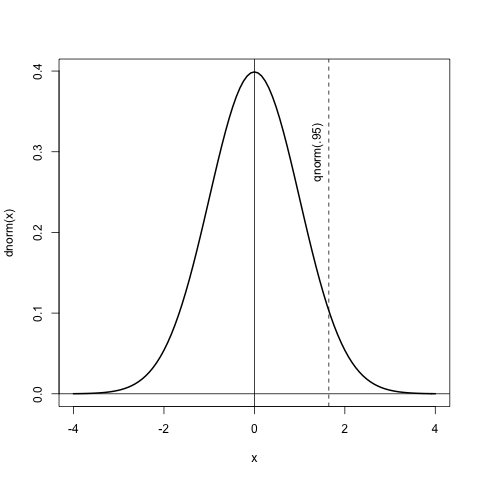
\includegraphics[scale=.45]{/export/WorkTree/Docus/Teaching/StatInf/Cours/td/img/N01corr.png}
\end{center}

\IndicR
\begin{Verbatim}[frame=leftline,fontfamily=tt,fontshape=n,numbers=left]
> yCA
  [1] 1 0 1 1 1 1 0 1 1 1 0 1 1 1 1 1 1 1 1 1 0 1 1 1 0 0 1 1 1 1 1 1 1 1 1 1 1
 [38] 1 1 0 1 0 1 1 1 1 1 1 1 0 1 1 1 0 1 0 1 1 1 0 0 1 1 1 1 1 1 1 1 1 1 1 1 1
...
[445] 1 1 1 0 1 1 1 1 1 0 1 0 1 1 1 1 1 1 1 1 1 1 1 1 1 1 1 0 1 1 1 1 0 0 1 1 1
[482] 1 1 1 1 1 1 1 0 1 1 1 1 1 1 1 1 1 1 1
> mean(yCA)
[1] 0.84
> # deltaEst.H0 <- (instruction R à fournir dans la rédaction)
> deltaEst.H0
[1] 2.236068
> pnorm(deltaEst.H0)
[1] 0.9873263
\end{Verbatim}

\begin{Correction}

\noindent \textbf{Hypothèses de test} : $\mathbf{H}_0:$ $p^{CA}=80\%$ vs {\large $\mathbf{H}_1:$ $p^{CA}>80\%$}\\
\textbf{Statistique de test sous $\mathbf{H}_0$} :
  $$
  \Est{\delta_{p^{CA},80\%}}{Y^{CA}}= {\displaystyle \frac{\Est{p^{CA}}{Y^{CA}}-80\%}{
\sqrt{\frac{80\%\times (1-80\%)} {500}}
}} 
  \SuitApprox \mathcal{N}(0,1)
  $$
\textbf{Règle de décision} : Accepter $\mathbf{H}_1$ si 
  p-valeur (droite) < 5\%\\
\noindent \textbf{Conclusion} :
puisqu'au vu des données, 
  \[
p-valeur\NotR\mathtt{1-pnorm((mean(yCA)-0.8)/sqrt(0.8*(1-0.8)/length(yCA)))} \simeq 1.27\% < 5\%,
\]
on peut plutôt penser (avec un risque de 5\%) que plus de 80\% de gens parmi la population cibl{\'e}e connaissent le produit~A.
\end{Correction}


\item M{\^e}me question avec un risque d'erreur de premi{\`e}re esp{\`e}ce pr{\'e}fix{\'e} {\`a} 1\%~?


 \begin{Correction}

\noindent \textbf{Hypothèses de test} : $\mathbf{H}_0:$ $p^{CA}=80\%$ vs {\large $\mathbf{H}_1:$ $p^{CA}>80\%$}\\
\textbf{Statistique de test sous $\mathbf{H}_0$} :
  $$
  \Est{\delta_{p^{CA},80\%}}{Y^{CA}}= {\displaystyle \frac{\Est{p^{CA}}{Y^{CA}}-80\%}{
\sqrt{\frac{80\%\times (1-80\%)} {500}}
}} 
  \SuitApprox \mathcal{N}(0,1)
  $$
\textbf{Règle de décision} : Accepter $\mathbf{H}_1$ si 
  p-valeur (droite) < 1\%\\
\noindent \textbf{Conclusion} :
puisqu'au vu des données, 
  \[
p-valeur\NotR\mathtt{1-pnorm((mean(yCA)-0.8)/sqrt(0.8*(1-0.8)/length(yCA)))} \simeq 1.27\%\nless1\%,
\]
on ne peut pas plutôt penser (avec un risque de 1\%) que plus de 80\% de gens parmi la population cibl{\'e}e connaissent le produit~A.
\end{Correction}



\end{enumerate}
\end{exercice}

\begin{exercice} (prime encouragement pour la qualité du produit A - contrôle continu 2003)

Comme chaque ann{\'e}e l'industriel afin d'encourager ses employ{\'e}s d{\'e}cide de leur verser une prime de fin d'ann{\'e}e si la client{\`e}le (potentielle) juge le produit~A de \textbf{bonne qualit{\'e}}. Sur une {\'e}chelle de valeurs  entre 0 et 10 mesurant le degr{\'e} de satisfaction, le produit est jug{\'e} de \textbf{bonne qualit{\'e}} si la note moyenne (sur les $N=2000000$ acheteurs potentiels), not{\'e}e $\mu^Q$, est strictement sup{\'e}rieure {\`a} 6 prouvant une qualit{\'e} plus qu'honorable de son produit.\\
\noindent \underline{Partie I (du point de vue de l'industriel)} (25 min.) \\

\begin{enumerate}
\item a) Exprimez l'assertion d'int{\'e}r{\^e}t conduisant {\`a} r{\'e}compenser les employ{\'e}s en fonction du param{\`e}tre d'int{\'e}r{\^e}t $\mu^Q$. \\


\begin{Correction}
L'assertion d'intérêt s'écrit : les employés sont récompensés si $\mu^Q>6$.
\end{Correction}


b) De quelles informations doit-on disposer pour {\'e}valuer le param{\`e}tre $\mu^Q$? Est-ce envisageable en pratique~?


\begin{Correction}
Pour connaître le paramètre $\mu^Q$, il faut disposer des réponses des $N$ consommateurs potentiels, ce qui n'est pas envisageable en pratique. 
\end{Correction}



Pour apporter un {\'e}l{\'e}ment de r{\'e}ponse, on d{\'e}cide d'interroger un {\'e}chantillon de 200 personnes. Chacun d'eux se prononce donc sur la qualit{\'e} du produit~A {\`a} travers une note de 0 {\`a} 10. En \texttt{R}, on stocke le jeu de donn{\'e}es $\Vect{y}^Q$ dans le vecteur \texttt{yQ}~:

\begin{Verbatim}[frame=leftline,fontfamily=tt,fontshape=n,numbers=left]
> yQ
  [1]  9  4  3  7  6  8  2  7  3  9  9  4  8  9  4  8 10  4  9  5  2  7  2  3  2
 [26]  4  9  6 10  8  5  5  5  5 10  7  4  4  4  4  6  8  2  8  9  5  7  8  6  4
...
[151]  7 10  6  5  4  9  5  6  4  2  6  7  5  6 10  8  6  5  9  7  2  2  2  8  9
[176]  6  3  8  7  6  3  8 10  2  2  8  9 10  9  8  2  7  7 10  3  3  2  9  7  6
\end{Verbatim}

 
\item a) D{\'e}crivez litt{\'e}ralement les deux erreurs de d{\'e}cision. 


\begin{Correction}
Erreur I : récompenser les employés alors que le produit n'est pas de bonne qualité. \\
Erreur II : ne pas récompenser les employés alors que le produit est de bonne qualité.
\end{Correction}


b) Pr{\'e}cisez pour quelle(s) valeur(s) du param{\`e}tre d'int{\'e}r{\^e}t $\mu^Q$ inconnu chacune de ces deux erreurs intervient. 


\begin{Correction}
L'erreur I intervient lorsque $\mu^Q\leq 6$ alors que l'erreur~II intervient lorsque $\mu^Q> 6$.
\end{Correction}


c) Quelle vous semble {\^e}tre la plus grave de ces deux erreurs \textbf{du point de vue de l'industriel}~? 


\begin{Correction}
Du point de vue de l'industriel, l'erreur I semble être la plus grave.
\end{Correction}



d) A votre avis autour de quelles valeurs de $\mu^Q$ la d{\'e}cision vous semblera-t-elle difficile {\`a} prendre (cette valeur constituera la pire des situations)~? 


\begin{Correction}
La décision semblera difficile à prendre autour de la valeur $6$ pour le paramètre $\mu^Q$.
\end{Correction}




\item Dans la pire des situations (i.e. lorsque $\mu^Q=6$), la mesure d'{\'e}cart standardis{\'e}e de test s'{\'e}crit~: 
$$
\Est{\delta_{\mu^Q,6}}{Y^Q} = \frac{ \Est{\mu^Q}{Y^Q} - 6 }{ \sqrt{ \frac{\Est{\sigma_Q^2}{Y^Q}}{200}}} \SuitApprox \mathcal{N}(0,1)
$$
Rappeler tr{\`e}s bri{\`e}vement comment on peut interpr{\'e}ter ce r{\'e}sultat via l'Approche Exp{\'e}rimentale. 


\begin{Correction}
Dans la pire des situations, imaginons pouvoir disposer d'une infinité de jeux de données notés $\Vect{y}_{[1]},\ldots,\Vect{y}_{[m]},\ldots$. Imaginons encore pouvoir calculer pour chacun de ces jeux de données expérimentaux l'estimation du paramètre d'écart standardisé $\Est{\delta_{\mu^Q,6}}{y_{[1]}}, \ldots, \Est{\delta_{\mu^Q,6}}{y_{[m]}},\ldots$. Le résultat énonce affirme que le contour supérieur de l'histogramme de l'infinité de ces estimations représentées par des briques devenues points correspond à la densité de probabilité (courbe lisse) d'une loi $\mathcal{N(0,1)}$. 
\end{Correction}



\item a) Si on ne souhaite exc{\'e}der 5\% de risque de d{\'e}cider {\`a} tort de r{\'e}compenser les employ{\'e}s, {\'e}tablir la r{\`e}gle de d{\'e}cision et conclure quant {\`a} la bonne qualit{\'e} du produit en vous aidant des quelques instructions \texttt{R}. \\
b) Concr{\`e}tement, quelle d{\'e}cision doit prendre l'industriel quant au versement de la prime de fin d'ann{\'e}e.

\IndicR
\begin{Verbatim}[frame=leftline,fontfamily=tt,fontshape=n,numbers=left]
> mean(yQ)
[1] 6.245
> sd(yQ)
[1] 2.458699
> # deltaEst.H0 <- (instruction R à fournir dans la rédaction)
> deltaEst.H0
[1] 1.40921
> pnorm(deltaEst.H0)
[1] 0.9206135
\end{Verbatim}

 

\begin{Correction}

\noindent \textbf{Hypothèses de test} : $\mathbf{H}_0:$ $\mu^{Q}=6$ vs {\large $\mathbf{H}_1:$ $\mu^{Q}>6$}\\
\textbf{Statistique de test sous $\mathbf{H}_0$} :
  $$
  \Est{\delta_{\mu^{Q},6}}{Y^{Q}}= {\displaystyle \frac{\Est{\mu^{Q}}{Y^{Q}}-6}{
\Est{\sigma_{\cqlshat{\mu^{Q}}}}{Y^{Q}}
}} 
  \SuitApprox \mathcal{N}(0,1)
  $$
\textbf{Règle de décision} : Accepter $\mathbf{H}_1$ si 
  p-valeur (droite) < 5\%\\
\noindent \textbf{Conclusion} :
puisqu'au vu des données, 
  \[
p-valeur\NotR\mathtt{1-pnorm((mean(yQ)-6)/seMean(yQ))} \simeq 7.94\%\nless5\%,
\]
on ne peut pas plutôt penser (avec un risque de 5\%) que les employés méritent la prime de fin d'année.
Concrètement, l'industriel déciderait sans doute de ne pas récompenser ses employés.
\end{Correction}



\end{enumerate}

\noindent \underline{Partie II (du point de vue des employ{\'e}s)} (25 min.) \\

Ind{\'e}pendamment des r{\'e}ponses pr{\'e}c{\'e}dentes un employ{\'e} ayant de solides connaissances en statistiques s'interroge sur le test pr{\'e}c{\'e}dent et notamment sur les deux risques d'erreur de d{\'e}cision mis en jeu. 

\begin{enumerate}
\item \textbf{Du point de vue des employ{\'e}s}, quelle est la plus grave des deux erreurs de d{\'e}cision dans le test pr{\'e}c{\'e}dent~?


\begin{Correction}
Du point de vue des employés, l'erreur la plus grave correspond à celle de ne pas être récompensé à tort.
\end{Correction}


\item En tant que d{\'e}l{\'e}gu{\'e}, un employé exprime alors au nom de ses coll{\`e}gues la revendication suivante~: ``nous acceptons de ne pas recevoir de prime de fin d'ann{\'e}e si vous pouvez prouver au vu du m{\^e}me jeu de donn{\'e}es pr{\'e}c{\'e}dent que le produit n'est pas de bonne qualit{\'e} (i.e. $\mu^Q<6$)''. Peut-on prouver au vu des donn{\'e}es que la note moyenne du degr{\'e} de satisfaction est strictement inf{\'e}rieure {\`a} 6~? (Indication~: r{\'e}daction standard et conclure en fournissant la valeur de la p$-$valeur)


\begin{Correction}

\noindent \textbf{Hypothèses de test} : $\mathbf{H}_0:$ $\mu^{Q}=6$ vs {\large $\mathbf{H}_1:$ $\mu^{Q}<6$}\\
\textbf{Statistique de test sous $\mathbf{H}_0$} :
  $$
  \Est{\delta_{\mu^{Q},6}}{Y^{Q}}= {\displaystyle \frac{\Est{\mu^{Q}}{Y^{Q}}-6}{
\Est{\sigma_{\cqlshat{\mu^{Q}}}}{Y^{Q}}
}} 
  \SuitApprox \mathcal{N}(0,1)
  $$
\textbf{Règle de décision} : Accepter $\mathbf{H}_1$ si 
  p-valeur (gauche) < 5\%\\
\noindent \textbf{Conclusion} :
puisqu'au vu des données, 
  \[
p-valeur\NotR\mathtt{pnorm((mean(yQ)-6)/seMean(yQ))} \simeq 92.06\%\nless5\%,
\]
on ne peut pas plutôt penser (avec un risque de 5\%) que les employés ne méritent pas la prime de fin d'année.
\end{Correction}
 

\item Ce d{\'e}l{\'e}gu{\'e} d{\'e}sireux d'approfondir son argumentation, pose la question suivante {\`a} l'industriel~: ``si on avait obtenu $\Est{\mu^Q}{y^Q}$ et $\Est{\sigma_{Q}}{y^Q}$ de l'ordre de 6.245 et 2.459 respectivement non pas avec la taille d'{\'e}chantillon actuelle de $n=200$ mais avec une taille plus grande, pensez-vous que vous auriez pu montrer que le produit {\'e}tait de bonne qualit{\'e}~?''\\
Et vous qu'en pensez-vous en vous aidant des instructions suivantes (en particulier si la taille d'{\'e}chantillon avait {\'e}t{\'e} $n=300$, $n=500$ et $n=1000$)~?

\begin{Verbatim}[frame=leftline,fontfamily=tt,fontshape=n,numbers=left]
> (mean(yQ)-6)/sqrt(var(yQ)/300)
[1] 1.725923
> pnorm((mean(yQ)-6)/sqrt(var(yQ)/1000))
[1] 0.9991867
\end{Verbatim}



\begin{Correction}
Pour $n=300$, on a $\Est{\delta_{\mu^Q,6}}{y^Q}\simeq 1.73>\delta_{lim,5\%}^+\simeq1.645$. Par conséquent, si les données n'avaient pas été obtenues avec $n=200$ mais avec $n=300$ on aurait plutôt pensé (avec un risque de 5\%) que les employés auraient dû être récompensés (i.e. on aurait accepté $\mathbf{H_1}: \mu^Q>6$). Même conclusion, pour $n=1000$, puisque p$-$valeur (droite)$\simeq 0.01\%<5\%$. Pour $n=500$ la conclusion aurait été identique puisque
$$
\frac{\Est{\mu^Q}{y^Q}-6}{ \frac{ \Est{\sigma^Q}{y^Q}}{\sqrt{500}} } > 
\frac{\Est{\mu^Q}{y^Q}-6}{ \frac{ \Est{\sigma^Q}{y^Q}}{\sqrt{300}} } > \delta_{lim,5\%}^+\simeq1.645
$$
\end{Correction}
 
\end{enumerate}
\end{exercice}

\begin{exercice} (compétence)
Un service de contr{\^o}le d'une entreprise de m{\'e}tallurgie s'int{\'e}resse {\`a} savoir si un technicien est suffisamment pr{\'e}cis au niveau des mesures quotidiennes qu'il effectue sur des minerais de fer (les mesures effectu{\'e}es sont des mesures de diam{\`e}tre). Une comp{\'e}tence ``suffisante'' que nous allons d{\'e}finir) sera r{\'e}compens{\'e}e par une prime. Le technicien sera d'autant plus précis que l'écart entre deux mesures d'un même minerai (sans qu'il le sache) est faible. Fort de constater que l'écart moyen est théoriquement nul (à justifier), la précision sera naturellement mesurée  par la variance des écarts. 

Soit $Y^C$  un futur écart entre deux mesures d'un même minerai. C'est une variable aléatoire qui est caractérisée (via l'approche expérimentale) par la donnée d'une infinité d'écarts virtuels (entre deux mesures) $y^C_{[1]},\ldots,y^C_{[m]},\ldots$. On notera $\sigma^2_C$ la variance de l'infinité de ces écarts de mesure qui constitue l'indicateur du niveau de précision du technicien. Cet indicateur  constitue le param{\`e}tre d'int{\'e}r{\^e}t de l'{\'e}tude. Le service de contr{\^o}le d{\'e}cide que le technicien est comp{\'e}tent (et pourra ainsi lui verser une prime) si le param{\`e}tre d'int{\'e}r{\^e}t est inf{\'e}rieur {\`a} $0.1$. \\

\begin{enumerate}

\item Au vu des données peut-on montrer que le technicien est compétent avec un risque d'erreur de première espèce fixé à 5\%.

\IndicR
\begin{Verbatim}[frame=leftline,fontfamily=tt,fontshape=n,numbers=left]
> yC
 [1]  0.34520624  0.36187714  0.28326083 -0.04273267  0.07897429 -0.57583456
 [7] -0.71994324  0.18188198  0.04438047 -0.01951828 -0.34820050  0.26067820
...
[25]  0.31212572  0.12692537 -0.17803505 -0.17861634 -0.48143225 -0.07185419
> var(yC)
[1] 0.08843689
> # deltaEst.H0 <- (instruction R à fournir dans la rédaction)
> deltaEst.H0
[1] -0.5474076
> pnorm(deltaEst.H0)
[1] 0.2920494
\end{Verbatim}

 

\begin{Correction}
\textbf{\underline{Option (préférée) correction AVEC p-valeur~:}}\\

\noindent \textbf{Hypothèses de test} : $\mathbf{H}_0:$ $\sigma^2_{C}=0.1$ vs {\large $\mathbf{H}_1:$ $\sigma^2_{C}<0.1$}\\
\textbf{Statistique de test sous $\mathbf{H}_0$} :
  $$
  \Est{\delta_{\sigma^2_{C},0.1}}{Y^{C}}= {\displaystyle \frac{\Est{\sigma^2_{C}}{Y^{C}}-0.1}{
\Est{\sigma_{\cqlshat{\sigma^2_{C}}}}{Y^{C}}
}} 
  \SuitApprox \mathcal{N}(0,1)
  $$
\textbf{Règle de décision} : Accepter $\mathbf{H}_1$ si 
  p-valeur (gauche) < 5\%\\
\noindent \textbf{Conclusion} :
puisqu'au vu des données, 
  \[
p-valeur\NotR\mathtt{pnorm((var(yC)-0.1)/seVar(yC))} \simeq 29.2\%\nless5\%,
\]
on ne peut pas plutôt penser (avec un risque de 5\%) que le technicien est compétent.

\textbf{\underline{Option correction SANS p-valeur~:}}\\

\noindent \textbf{Hypothèses de test} : $\mathbf{H}_0:$ $\sigma^2_{C}=0.1$ vs {\large $\mathbf{H}_1:$ $\sigma^2_{C}<0.1$}\\
\textbf{Statistique de test sous $\mathbf{H}_0$} :
  $$
  \Est{\delta_{\sigma^2_{C},0.1}}{Y^{C}}= {\displaystyle \frac{\Est{\sigma^2_{C}}{Y^{C}}-0.1}{
\Est{\sigma_{\cqlshat{\sigma^2_{C}}}}{Y^{C}}
}} 
  \SuitApprox \mathcal{N}(0,1)
  $$
\textbf{Règle de décision} : Accepter $\mathbf{H}_1$ si 
  $\Est{\delta_{\sigma^2_{C},0.1}}{y^{C}} < \delta^-_{lim,5\%}$\\
\noindent \textbf{Conclusion} :
puisqu'au vu des données, 
  \begin{eqnarray*}
\Est{\delta_{\sigma^2_{C},0.1}}{y^{C}} &\NotR&\mathtt{(var(yC)-0.1)/seVar(yC)}\simeq -0.5474076\\&\nless & \delta^-_{lim,5\%} \NotR \mathtt{-qnorm(1-.05)}\simeq-1.644854
\end{eqnarray*}
  
on ne peut pas plutôt penser (avec un risque de 5\%) que le technicien est compétent.
\end{Correction}


\item Le service de contr{\^o}le ({\`a} qui on a fait comprendre que le risque $\alpha$ est g{\'e}n{\'e}ralement fix{\'e} {\`a} $5\%$) d{\'e}cide au vu de la p-valeur du pr{\'e}c{\'e}dent test de renvoyer sur le champ le technicien. Ce dernier bien plus au courant des techniques statistiques assigne son employeur aux prud'hommes et gagne le proc{\`e}s haut la main. L'argument avanc{\'e} par le technicien est le suivant : ``Le service de contr{\^o}le n'a en aucun cas prouv{\'e} que je n'{\'e}tais pas comp{\'e}tent. Il n'a seulement pas pu prouver au vu des donn{\'e}es que j'{\'e}tais comp{\'e}tent : soit il prouve que je ne suis pas comp{\'e}tent, soit il me soumet {\`a} un nombre plus {\'e}lev{\'e} d'{\'e}chantillons de mani{\`e}re {\`a} ce que l'estimation de la variance soit significative.''. Essayez de traduire math{\'e}matiquement l'argument du technicien. 


\begin{Correction}
La conclusion du précédent test n'autorise pas le service de contrôle à penser que le technicien n'est pas compétent. Pour pouvoir montrer ceci il doit effectuer le test suivant~: $\mathbf{H_1}: \sigma_C^2>0.1$. Or, $\Est{\delta_{\sigma_C^2,0.1}}{y^C}\simeq -0.5474 \ngtr \delta_{lim,5\%}^+\simeq 1.645$. En conclusion, on ne peut vraiment rien dire au vu des données (avec un risque de 5\%)!
\end{Correction}


\item Le service de contr{\^o}le d{\'e}cide alors de soumettre deux fois le technicien {\`a} $n=500$ mesures sur les {\'e}chantillons de minerai. Le vecteur des 500 {\'e}carts de mesures est encore not{\'e} ${\bf y}^C$. Avec ces nouvelles observations que concluez-vous au seuil de $5 \%$ ? \\

\IndicR
\begin{Verbatim}[frame=leftline,fontfamily=tt,fontshape=n,numbers=left]
> yC
  [1]  0.345206239  0.361877141  0.283260829 -0.042732674  0.078974292
  [6] -0.575834563 -0.719943239  0.181881984  0.044380473 -0.019518279
...
[491] -0.070185269  0.134088213  0.277789013 -0.079484256 -0.107560964
[496] -0.265767699 -0.124663757 -0.026684338  0.494449721 -0.304572345
> var(yC)
[1] 0.08299474
> # deltaEst.H0 <- (instruction R à fournir dans la rédaction)
> deltaEst.H0
[1] -3.299262
> pnorm(deltaEst.H0)
[1] 0.0004846965
\end{Verbatim}

 

\begin{Correction}

\noindent \textbf{Assertion d'intérêt} :  $\mathbf{H}_1:$ $\sigma^2_{C}<0.1$ \\
\textbf{Application numérique} :  puisqu'au vu des données, 
  \[
p-valeur\NotR\mathtt{pnorm((var(yC)-0.1)/seVar(yC))} \simeq 0.05\% < 5\%,
\]
on peut plutôt penser (avec un risque de 5\%) que le technicien est compétent.
\end{Correction}

\end{enumerate}
\end{exercice}

\begin{exercice}(diététicien)
Un di{\'e}t{\'e}ticien affirme que son r{\'e}gime alimentaire permet une perte de poids rapide. On observe la r{\'e}partition d'un {\'e}chantillon de $10$ femmes ayant suivi ce r{\'e}gime pendant $2$ semaines.
$$
\begin{tabular}{|c|c|c|c|c|c|c|c|c|c|c|}\hline
{\bf Poids avant AV} &
$64$ & $67$ & $68$ & $76$ & $72$ & $69$ & $62$ & $65$ & $64$ & $73$ \\\hline
{\bf Poids apr{\`e}s AP} &
$65$ & $61$ & $64$ & $69$ & $65$ & $66$ & $60$ & $59$ & $61$ & $68$ \\\hline
{\bf Perte de poids $Y$} &
$-1$ & $6$ & $4$ & $7$ & $7$ & $3$ & $2$ & $6$ & $3$ & $5$ \\\hline
\end{tabular}
$$

\textit{Voici les donn{\'e}es pr{\'e}liminairement saisies et plac{\'e}es dans deux vecteurs $\Vect{AV}$ et $\Vect{AP}$. Le vecteur $\Vect{y}$ est obtenu en faisant une diff{\'e}rence {\'e}l{\'e}ment par {\'e}l{\'e}ment}~:

\IndicR
\begin{Verbatim}[frame=leftline,fontfamily=tt,fontshape=n,numbers=left]
> AV-AP
 [1] -1  6  4  7  7  3  2  6  3  5
> mean(AV-AP)
[1] 4.2
> sd(AV-AP)
[1] 2.529822
> seMean(AV-AP)
[1] 0.8
\end{Verbatim}


1. En supposant que $Y\leadsto N\left( \mu ,\sigma \right) $, {\'e}prouver
l'affirmation du di{\'e} t{\'e}ticien au seuil de signification $5\%$.

\IndicR
\begin{Verbatim}[frame=leftline,fontfamily=tt,fontshape=n,numbers=left]
> # deltaEst.H0 <- (instruction R à fournir dans la rédaction)
> deltaEst.H0
[1] 5.25
> pt(deltaEst.H0,9)
[1] 0.9997362
\end{Verbatim}


\begin{Correction}
\noindent \textbf{Préliminaire}~: puisque  $\mathtt{(mean(AV-AP)-0)}\simeq4.2$ est du même signe (i.e. positif que $\mathtt{deltaEst.H0}$ (car p-valeur gauche supérieure à $50\%$), on a~:
    \begin{itemize}
\item \textit{variable d'intérêt}~: $Y^{D}=Y^{AV}-Y^{AP}$
\item \textit{paramètre d'intérêt}~: $\mu^{D}=\mbox{``moyenne de $Y^{D}$"}=\mu^{AV}-\mu^{AP}$
\end{itemize}
\noindent \textbf{Hypothèses de test} : $\mathbf{H}_0:$ $\mu^{D}=0$ vs {\large $\mathbf{H}_1:$ $\mu^{D}>0$}\\
\textbf{Statistique de test sous $\mathbf{H}_0$} :
  $$
  \Est{\delta_{\mu^{D},0}}{Y^{D}}= {\displaystyle \frac{\Est{\mu^{D}}{Y^{D}}-0}{
\Est{\sigma_{\cqlshat{\mu^{D}}}}{Y^{D}}
}} 
  \leadsto \mathcal{S}t(10-1)
  $$
\textbf{Règle de décision} : Accepter $\mathbf{H}_1$ si 
  p-valeur (droite) < 5\%\\
\noindent \textbf{Conclusion} :
puisqu'au vu des données, 
  \[
p-valeur\NotR\mathtt{1-pt((mean(AV-AP)-0)/seMean(AV-AP),9)} \simeq 0.03\% < 5\%,
\]
on peut plutôt penser (avec un risque de 5\%) que le régime alimentaire du diététicien permet une perte de poids.
\end{Correction}


2. Fort de ce constat, le di{\'e}t{\'e}ticien aimerait un titre plus accrocheur et souhaiterait montrer avec le m{\^e}me jeu de donn{\'e}es $\Vect{y}$ que son r{\'e}gime permet une perte de deux kilos par semaine. {\'E}prouvez cette nouvelle affirmation au seuil de 5\%.

\IndicR
\begin{Verbatim}[frame=leftline,fontfamily=tt,fontshape=n,numbers=left]
> # deltaEst.H0 <- (instruction R à fournir dans la rédaction)
> deltaEst.H0
[1] 0.25
> pt(deltaEst.H0,9)
[1] 0.5958998
\end{Verbatim}


\begin{Correction}
\noindent \textbf{Préliminaire}~: puisque  $\mathtt{(mean(AV-AP)-4)}\simeq0.2$ est du même signe (i.e. positif que $\mathtt{deltaEst.H0}$ (car p-valeur gauche supérieure à $50\%$), on a~:
    \begin{itemize}
\item \textit{variable d'intérêt}~: $Y^{D}=Y^{true}-Y^{AP}$
\item \textit{paramètre d'intérêt}~: $\mu^{D}=\mbox{``moyenne de $Y^{D}$"}=\mu^{true}-\mu^{AP}$
\end{itemize}
\noindent \textbf{Hypothèses de test} : $\mathbf{H}_0:$ $\mu^{D}=4$ vs {\large $\mathbf{H}_1:$ $\mu^{D}>4$}\\
\textbf{Statistique de test sous $\mathbf{H}_0$} :
  $$
  \Est{\delta_{\mu^{D},4}}{Y^{D}}= {\displaystyle \frac{\Est{\mu^{D}}{Y^{D}}-4}{
\Est{\sigma_{\cqlshat{\mu^{D}}}}{Y^{D}}
}} 
  \leadsto \mathcal{S}t(10-1)
  $$
\textbf{Règle de décision} : Accepter $\mathbf{H}_1$ si 
  p-valeur (droite) < 5\%\\
\noindent \textbf{Conclusion} :
puisqu'au vu des données, 
  \[
p-valeur\NotR\mathtt{1-pt((mean(AV-AP)-4)/seMean(AV-AP),9)} \simeq 40.41\%\nless5\%,
\]
on ne peut pas plutôt penser (avec un risque de 5\%) que le régime alimentaire du diététicien permet une perte de poids de 2 kilos par semaine.
\end{Correction}



3. Pas d{\'e}sappoint{\'e} pour autant par la pr{\'e}c{\'e}dente analyse, le di{\'e}t{\'e}ticien d{\'e}cide de soumettre 40 femmes suppl{\'e}mentaires {\`a} son r{\'e}gime, et compl{\`e}te ainsi son pr{\'e}c{\'e}dent vecteur $\Vect{y}$ correspondant aux pertes de poids. Il obtient finalement le jeu de donn{\'e}es suivant~:

\IndicR
\begin{Verbatim}[frame=leftline,fontfamily=tt,fontshape=n,numbers=left]
> yD
 [1] -1  6  4  7  7  3  2  6  3  5  5  7  4  4  2  4  6  6  5  3  5  5  2  7  4
[26]  5  4  3  6  7  4  6  4  5  2  6  4  6  5  5  6  4  3  2  3  6  5  7  2  4
> mean(yD)
[1] 4.5
> sd(yD)
[1] 1.729103
> seMean(yD)
[1] 0.244532
\end{Verbatim}
 
 
a) que pensez-vous alors de l'hypoth{\`e}se faite pr{\'e}c{\'e}demment affirmant~: $Y\leadsto N\left( \mu ,\sigma \right) $~?


\begin{Correction}
Cette hypothèse n'est plus nécessaire car on dispose maintenant de suffisamment de données pour que les résultats dans le cadre asymptotique soient valides.
\end{Correction}


b) pensez-vous avec ce nouveau jeu de donn{\'e}es que la nouvelle affirmation du di{\'e}t{\'e}ticien est vraie ({\`a} un risque d'erreur de premi{\`e}re esp{\`e}ce fix{\'e} {\`a} 5\%)~?

\IndicR
\begin{Verbatim}[frame=leftline,fontfamily=tt,fontshape=n,numbers=left]
> # deltaEst.H0 <- (instruction R à fournir dans la rédaction)
> deltaEst.H0
[1] 2.044722
> pnorm(deltaEst.H0)
[1] 0.9795589
\end{Verbatim}


\begin{Correction}

\noindent \textbf{Hypothèses de test} : $\mathbf{H}_0:$ $\mu^{D}=4$ vs {\large $\mathbf{H}_1:$ $\mu^{D}>4$}\\
\textbf{Statistique de test sous $\mathbf{H}_0$} :
  $$
  \Est{\delta_{\mu^{D},4}}{Y^{D}}= {\displaystyle \frac{\Est{\mu^{D}}{Y^{D}}-4}{
\Est{\sigma_{\cqlshat{\mu^{D}}}}{Y^{D}}
}} 
  \SuitApprox \mathcal{N}(0,1)
  $$
\textbf{Règle de décision} : Accepter $\mathbf{H}_1$ si 
  p-valeur (droite) < 5\%\\
\noindent \textbf{Conclusion} :
puisqu'au vu des données, 
  \[
p-valeur\NotR\mathtt{1-pnorm((mean(yD)-4)/seMean(yD))} \simeq 2.04\% < 5\%,
\]
on peut plutôt penser (avec un risque de 5\%) que le régime alimentaire du diététicien permet une perte de poids de 2 kilos par semaine.
\end{Correction}



c) Qu'expriment les erreurs standard (\texttt{seMean(y)}) pour $n=10$ et $n=50$~? Expliquez alors pourquoi on a pu accepter l'assertion d'intérêt du diététicien pour $n=50$.


\begin{Correction}
L'erreur standard $\Est{\sigma_{\widehat{\mu^D}}}{y^D}$ calculé en \texttt{R} par l'instruction \texttt{seMean(y)} mesure la qualité estimée (à partir du jeu de données de taille $n=10$ ou $50$) du remplaçant du paramètre d'intérêt $\mu^D$. On pourra noter que pour le jeu de données initial de taille $n=10$ on a $\Est{\mu^D}{y^D} =4.2$ et $\Est{\sigma_{\widehat{\mu^D}}}{y^D}=0.8$ et que pour le jeu de données complété de taille $n=50$, $\Est{\mu^D}{y^D} =4.5$ et $\Est{\sigma_{\widehat{\mu^D}}}{y^D}\simeq 0.24$. Ainsi, on peut remarquer qu'avec les deux jeux de données les estimations du paramètre d'intérêt sont sensiblement équivalentes, en revanche la seconde estimation semble à peu près trois fois plus précise que la première. C'est la raison pour laquelle l'assertion d'intérêt a pu être acceptée (avec un risque de 5\%) au vu du jeu de données complété.
\end{Correction}

\end{exercice}

\begin{exercice}

Un pilote de course en Formule 1 hésite entre deux équipes. Il fait alors des essais dans chacune des deux équipes pour savoir laquelle est la plus performante.\\

\noindent 1) Pour l'équipe 1, le pilote commence par faire 20 premiers tours. Les données des temps effectués par tour sont exprimées en secondes et stockées dans le vecteur  \texttt{y1}. Au vu des données peut-on montrer que le temps moyen de la voiture de l'équipe 1 est inférieur à 51 secondes  avec un risque d'erreur de première espèce fixé à 5\%~?\\

\IndicR
\begin{Verbatim}[frame=leftline,fontfamily=tt,fontshape=n,numbers=left]
> mean(y1)
[1] 50.21973
> sd(y1)
[1] 2.276776
> # deltaEst.H0 <- (instruction R à fournir dans la rédaction)
> deltaEst.H0
[1] -1.532634
> pt(deltaEst.H0,19)
[1] 0.07092418
\end{Verbatim}


\begin{Correction}

\noindent \textbf{Hypothèses de test} : $\mathbf{H}_0:$ $\mu^{E1}=51$ vs {\large $\mathbf{H}_1:$ $\mu^{E1}<51$}\\
\textbf{Statistique de test sous $\mathbf{H}_0$} :
  $$
  \Est{\delta_{\mu^{E1},51}}{Y^{E1}}= {\displaystyle \frac{\Est{\mu^{E1}}{Y^{E1}}-51}{
\Est{\sigma_{\cqlshat{\mu^{E1}}}}{Y^{E1}}
}} 
  \leadsto \mathcal{S}t(20-1)
  $$
\textbf{Règle de décision} : Accepter $\mathbf{H}_1$ si 
  p-valeur (gauche) < 5\%\\
\noindent \textbf{Conclusion} :
puisqu'au vu des données, 
  \[
p-valeur\NotR\mathtt{pt((mean(y1)-51)/seMean(y1),19)} \simeq 7.09\%\nless5\%,
\]
on ne peut pas plutôt penser (avec un risque de 5\%) que le temps moyen de la voiture de l'équipe 1 est inférieur à 51 secondes.
\end{Correction}



\noindent 2) Le pilote effectue 20 tours supplémentaires (les données sont toujours stockées dans le vecteur \texttt{y1}).
Même question que précédemment avec ce nouveau jeu de données complétées.\\
\IndicR
\begin{Verbatim}[frame=leftline,fontfamily=tt,fontshape=n,numbers=left]
> y1
 [1] 47.89674 50.04087 54.53240 54.36718 48.80645 51.44077 49.72669 44.81843
 [9] 50.37910 48.32037 53.55150 50.38611 50.37899 49.44585 50.47262 50.66881
...
[33] 48.83423 51.93978 49.19886 52.67034 49.21360 48.35678 49.43116 48.95199
> mean(y1)
[1] 50.39458
> sd(y1)
[1] 1.965069
> # deltaEst.H0 <- (instruction R à fournir dans la rédaction)
> deltaEst.H0
[1] -1.948534
> pnorm(deltaEst.H0)
[1] 0.02567557
\end{Verbatim}



\begin{Correction}

\noindent \textbf{Hypothèses de test} : $\mathbf{H}_0:$ $\mu^{E1}=51$ vs {\large $\mathbf{H}_1:$ $\mu^{E1}<51$}\\
\textbf{Statistique de test sous $\mathbf{H}_0$} :
  $$
  \Est{\delta_{\mu^{E1},51}}{Y^{E1}}= {\displaystyle \frac{\Est{\mu^{E1}}{Y^{E1}}-51}{
\Est{\sigma_{\cqlshat{\mu^{E1}}}}{Y^{E1}}
}} 
  \SuitApprox \mathcal{N}(0,1)
  $$
\textbf{Règle de décision} : Accepter $\mathbf{H}_1$ si 
  $\Est{\delta_{\mu^{E1},51}}{y^{E1}} < \delta^-_{lim,5\%}$\\
\noindent \textbf{Conclusion} :
puisqu'au vu des données, 
  \begin{eqnarray*}
\Est{\delta_{\mu^{E1},51}}{y^{E1}} &\NotR&\mathtt{(mean(y1)-51)/seMean(y1)}\simeq -1.948534\\& <  & \delta^-_{lim,5\%} \NotR \mathtt{-qnorm(1-.05)}\simeq-1.644854
\end{eqnarray*}
  
on peut plutôt penser (avec un risque de 5\%) que le temps moyen de la voiture de l'équipe 1 est inférieur à 51 secondes.
\end{Correction}


\noindent 3) Avec la voiture de l'équipe~2,  le pilote effectue 50 tours. Les données des temps effectués par tour sont exprimées en secondes et stockées dans le vecteur  \texttt{y2}. Au vu des données peut-on montrer que le temps moyen de la voiture de l'équipe 2 est inférieur à 51 secondes  avec un risque d'erreur de première espèce fixé à 5\%~?\\

\IndicR
\begin{Verbatim}[frame=leftline,fontfamily=tt,fontshape=n,numbers=left]
> y2
 [1] 51.89371 51.35814 52.16305 51.83228 52.97653 51.43513 50.89370 51.50756
 [9] 51.54468 52.22917 51.21122 52.96252 51.61797 52.40225 50.21097 51.73468
...
[49] 53.55974 52.44708
> mean(y2)
[1] 52.02422
> sd(y2)
[1] 0.8670206
> # deltaEst.H0 <- (instruction R à fournir dans la rédaction)
> deltaEst.H0
[1] 8.353126
> pnorm(deltaEst.H0)
[1] 1
\end{Verbatim}



\begin{Correction}

\noindent \textbf{Hypothèses de test} : $\mathbf{H}_0:$ $\mu^{E2}=51$ vs {\large $\mathbf{H}_1:$ $\mu^{E2}<51$}\\
\textbf{Statistique de test sous $\mathbf{H}_0$} :
  $$
  \Est{\delta_{\mu^{E2},51}}{Y^{E2}}= {\displaystyle \frac{\Est{\mu^{E2}}{Y^{E2}}-51}{
\Est{\sigma_{\cqlshat{\mu^{E2}}}}{Y^{E2}}
}} 
  \SuitApprox \mathcal{N}(0,1)
  $$
\textbf{Règle de décision} : Accepter $\mathbf{H}_1$ si 
  p-valeur (gauche) < 5\%\\
\noindent \textbf{Conclusion} :
puisqu'au vu des données, 
  \[
p-valeur\NotR\mathtt{pnorm((mean(y2)-51)/seMean(y2))} \simeq 100.0\%\nless5\%,
\]
on ne peut pas plutôt penser (avec un risque de 5\%) que le temps moyen de la voiture de l'équipe 2 est inférieur à 51 secondes.
\end{Correction}


\noindent 4) Quel est l'ordre de grandeur de la p$-$valeur du précédent test~? Donc à la vue des sorties R précédentes, les données permettent-elles de laisser penser qu'une certaine assertion d'intérêt (à préciser) est vraie~?



\begin{Correction}

\noindent \textbf{Assertion d'intérêt} :  $\mathbf{H}_1:$ $\mu^{E2}>51$ \\
\textbf{Application numérique} :  puisqu'au vu des données, 
  \[
p-valeur\NotR\mathtt{1-pnorm((mean(y2)-51)/seMean(y2))} \simeq 0.0\% < 5\%,
\]
on peut plutôt penser (avec un risque de 5\%) que le temps moyen de la voiture de l'équipe 2 est supérieur à 51 secondes.
\end{Correction}


\noindent 5) Au vu des données peut-on montrer que le temps moyen de l'équipe~1 est inférieur à celui de l'équipe~2  avec un risque d'erreur de première espèce fixé à 5\%~?\\
Cela est-il surprenant au regard le la conclusion de la question précédente~?\\
\IndicR
\begin{Verbatim}[frame=leftline,fontfamily=tt,fontshape=n,numbers=left]
> # deltaEst.H0 <- (instruction R à fournir dans la rédaction)
> deltaEst.H0
[1] -4.878811
\end{Verbatim}



\begin{Correction}
\noindent \textbf{Préliminaire} : puisque $\mathtt{(mean(y1)-mean(y2)-0)}\simeq-1.629639$ est du même signe (i.e. négatif) que $\mathtt{deltaEst.H0}$ , on a~: 
      \begin{itemize}
\item \textit{paramètre d'intérêt}~: $d_\mu=\mu^{E1}-\mu^{E2}$
\item \textit{sa future estimation}~: $\Est{d_\mu}{Y^{E1},Y^{E2}}=\Est{\mu^{E1}}{Y^{E1}}-\Est{\mu^{E2}}{Y^{E2}}$
\end{itemize}
\noindent \textbf{Hypothèses de test} : $\mathbf{H}_0:$ $d_\mu=0$ vs {\large $\mathbf{H}_1:$ $d_\mu<0$}\\
\textbf{Statistique de test sous $\mathbf{H}_0$} :
  $$
  \Est{\delta_{d_\mu,0}}{Y^{E1},Y^{E2}}= {\displaystyle \frac{\Est{d_\mu}{Y^{E1},Y^{E2}}-0}{
\Est{\sigma_{\cqlshat{d_\mu}}}{Y^{E1},Y^{E2}}
}} 
  \SuitApprox \mathcal{N}(0,1)
  $$
\textbf{Règle de décision} : Accepter $\mathbf{H}_1$ si 
  $\Est{\delta_{d_\mu,0}}{y^{E1},y^{E2}} < \delta^-_{lim,5\%}$\\
\noindent \textbf{Conclusion} :
puisqu'au vu des données, 
  \begin{eqnarray*}
\Est{\delta_{d_\mu,0}}{y^{E1},y^{E2}} &\NotR&\mathtt{(mean(y1)-mean(y2)-0)/seDMean(y1,y2)}\simeq -4.878811\\& <  & \delta^-_{lim,5\%} \NotR \mathtt{-qnorm(1-.05)}\simeq-1.644854
\end{eqnarray*}
  
on peut plutôt penser (avec un risque de 5\%) que le temps moyen de l'équipe~1 est inférieur à celui de l'équipe~2.

Cela n'est pas surprenant au regard des questions précédentes puisque nous avions conclu que l'on pouvait plutôt penser que le temps de l'équipe~1 (resp.~2) était inférieur (resp. supérieur) à 51 secondes. 
\end{Correction}


\noindent 6) Au vu des données peut-on montrer que la variance des temps de l'équipe~2 est inférieure à celle de l'équipe~1  avec un risque d'erreur de première espèce fixé à 5\%~?\\
\IndicR
\begin{Verbatim}[frame=leftline,fontfamily=tt,fontshape=n,numbers=left]
> # deltaEst.H0 <- (instruction R à fournir dans la rédaction)
> deltaEst.H0
[1] 3.161661
\end{Verbatim}



\begin{Correction}
\noindent \textbf{Préliminaire} : puisque $\mathtt{(var(y1)-var(y2)-0)}\simeq3.109772$ est du même signe (i.e. positif) que $\mathtt{deltaEst.H0}$ , on a~: 
      \begin{itemize}
\item \textit{paramètre d'intérêt}~: $d_{\sigma^2}=\sigma^2_{E1}-\sigma^2_{E2}$
\item \textit{sa future estimation}~: $\Est{d_{\sigma^2}}{Y^{E1},Y^{E2}}=\Est{\sigma^2_{E1}}{Y^{E1}}-\Est{\sigma^2_{E2}}{Y^{E2}}$
\end{itemize}
\noindent \textbf{Hypothèses de test} : $\mathbf{H}_0:$ $d_{\sigma^2}=0$ vs {\large $\mathbf{H}_1:$ $d_{\sigma^2}>0$}\\
\textbf{Statistique de test sous $\mathbf{H}_0$} :
  $$
  \Est{\delta_{d_{\sigma^2},0}}{Y^{E1},Y^{E2}}= {\displaystyle \frac{\Est{d_{\sigma^2}}{Y^{E1},Y^{E2}}-0}{
\Est{\sigma_{\cqlshat{d_{\sigma^2}}}}{Y^{E1},Y^{E2}}
}} 
  \SuitApprox \mathcal{N}(0,1)
  $$
\textbf{Règle de décision} : Accepter $\mathbf{H}_1$ si 
  $\Est{\delta_{d_{\sigma^2},0}}{y^{E1},y^{E2}} > \delta^+_{lim,5\%}$\\
\noindent \textbf{Conclusion} :
puisqu'au vu des données, 
  \begin{eqnarray*}
\Est{\delta_{d_{\sigma^2},0}}{y^{E1},y^{E2}} &\NotR&\mathtt{(var(y1)-var(y2)-0)/seDVar(y1,y2)}\simeq 3.161661\\& >  & \delta^+_{lim,5\%} \NotR \mathtt{qnorm(1-.05)}\simeq1.644854
\end{eqnarray*}
  
on peut plutôt penser (avec un risque de 5\%) que la variance des temps de l'équipe~2 est inférieure à celle de l'équipe~1.
\end{Correction}


\noindent 7) Exprimez littéralement les deux conclusions des deux tests précédents. Si vous étiez le pilote, quelle équipe choisiriez-vous~?


\begin{Correction}
Au regard des deux questions précédentes, on peut plutôt penser au vu des données que la voiture de l'équipe~1 est plus performante (en moyenne) que celle de l'équipe~2. En revanche cette dernière est plus régulière que la voiture de l'équipe~1. Le choix entre les deux équipes est donc un choix à faire entre performance moyenne et régularité. 
\end{Correction}


\end{exercice}

\begin{exercice} (1h - environ 10 pts)

\noindent \underline{Partie I: compétence d'un technicien} \\

Un service de contr{\^o}le d'une entreprise de m{\'e}tallurgie s'int{\'e}resse {\`a} savoir si un technicien (Alfred) est suffisamment pr{\'e}cis au niveau des mesures qu'il effectue sur des minerais de fer. Le technicien sera d'autant plus précis que l'écart entre deux mesures d'un même minerai (sans qu'il le sache) est faible. La précision serait théoriquement mesurée  par la variance d'une infinité d'écarts entre deux mesures. On notera $\sigma^2_A$ (comme Alfred) cette variance.  Le service de contr{\^o}le d{\'e}cide qu'un technicien est comp{\'e}tent si ce param{\`e}tre d'int{\'e}r{\^e}t est inf{\'e}rieur {\`a} $0.1$. \\ 

\begin{enumerate}
\item On commence par soumettre Alfred à $n^A=20$ échantillons de minerai de fer. Le jeu de données est stocké dans le vecteur \texttt{yA} dans \texttt{R}. Peut-on montrer au seuil de $5\%$ qu'Alfred est compétent~? (précisez l'hypothèse mathématique faite sur la nature des données)

\IndicR
\begin{Verbatim}[frame=leftline,fontfamily=tt,fontshape=n,numbers=left]
> yA
 [1]  0.14467956  0.30839102  0.16507184  0.08100885 -0.15048984 -0.02163446
 [7] -0.25558794  0.09871536  0.59275135 -0.22962500 -0.21676732 -0.09707208
[13]  0.17050529 -0.05732366  0.65337514  0.17802469  0.29278735 -0.16514972
[19] -0.30080221  0.32129752
> var(yA)
[1] 0.07325571
> sd(yA)
[1] 0.2706579
> # deltaEst.H0 <- (instruction R à fournir dans la rédaction)
> deltaEst.H0
[1] 13.91858
> qchisq(c(0.01,0.025,0.05,0.1,0.9,0.95,0.975,0.99),19)
[1]  7.632730  8.906516 10.117013 11.650910 27.203571 30.143527 32.852327
[8] 36.190869
> pchisq(deltaEst.H0,19)
[1] 0.2115835
\end{Verbatim}



\begin{Correction}

\noindent \textbf{Hypothèses de test} : $\mathbf{H}_0:$ $\sigma^2_{A}=0.1$ vs {\large $\mathbf{H}_1:$ $\sigma^2_{A}<0.1$}\\
\textbf{Statistique de test sous $\mathbf{H}_0$} :
  $$
  \Est{\delta_{\sigma^2_{A},0.1}}{Y^{A}}= {\displaystyle (20-1)\frac{\Est{\sigma^2_{A}}{Y^{A}}}{0.1}} 
  \leadsto \chi^2(20-1)
  $$
\textbf{Règle de décision} : Accepter $\mathbf{H}_1$ si 
  p-valeur (gauche) < 5\%\\
\noindent \textbf{Conclusion} :
puisqu'au vu des données, 
  \[
p-valeur\NotR\mathtt{pchisq((length(yA)-1)*var(yA)/0.1,19)} \simeq 21.16\%\nless5\%,
\]
on ne peut pas plutôt penser (avec un risque de 5\%) que Alfred est compétent.
\end{Correction}


\item On complète le jeu de données précédent en soumettant le technicien à 30 \textbf{nouveaux} échantillons. Le jeu de données est toujours stocké dans le vecteur \texttt{yA}. Peut-on maintenant montrer au seuil de $5\%$ que le technicien est compétent~?

\IndicR
\begin{Verbatim}[frame=leftline,fontfamily=tt,fontshape=n,numbers=left]
> yA
 [1]  0.144679564  0.308391020  0.165071844  0.081008851 -0.150489836
 [6] -0.021634458 -0.255587943  0.098715356  0.592751352 -0.229624997
...
[41]  0.262084534 -0.215753300  0.173626815 -0.200160681 -0.255138748
[46]  0.125329351 -0.326049545  0.207517750  0.070438920 -0.303221493
> var(yA)
[1] 0.06362229
> sd(yA)
[1] 0.2522346
> # deltaEst.H0 <- (instruction R à fournir dans la rédaction)
> deltaEst.H0
[1] -2.762438
> pnorm(deltaEst.H0)
[1] 0.002868572
\end{Verbatim}



\begin{Correction}

\noindent \textbf{Hypothèses de test} : $\mathbf{H}_0:$ $\sigma^2_{A}=0.1$ vs {\large $\mathbf{H}_1:$ $\sigma^2_{A}<0.1$}\\
\textbf{Statistique de test sous $\mathbf{H}_0$} :
  $$
  \Est{\delta_{\sigma^2_{A},0.1}}{Y^{A}}= {\displaystyle \frac{\Est{\sigma^2_{A}}{Y^{A}}-0.1}{
\Est{\sigma_{\cqlshat{\sigma^2_{A}}}}{Y^{A}}
}} 
  \SuitApprox \mathcal{N}(0,1)
  $$
\textbf{Règle de décision} : Accepter $\mathbf{H}_1$ si 
  p-valeur (gauche) < 5\%\\
\noindent \textbf{Conclusion} :
puisqu'au vu des données, 
  \[
p-valeur\NotR\mathtt{pnorm((var(yA)-0.1)/seVar(yA))} \simeq 0.29\% < 5\%,
\]
on peut plutôt penser (avec un risque de 5\%) que Alfred est compétent.
\end{Correction}

\end{enumerate}

\noindent \underline{Partie II : comparaison de deux techniciens} \\

\begin{enumerate}

\item On s'intéresse à un second technicien (Bernard) dont on cherche à montrer qu'il est compétent. Bernard a été soumis à $n^B=20$ échantillons de minerai; les données relatives à ses écarts de mesure sont stockées en \texttt{R} dans le vecteur \texttt{yB}. Peut-on montrer qu'il est compétent au seuil de 5\%~?


\IndicR
\begin{Verbatim}[frame=leftline,fontfamily=tt,fontshape=n,numbers=left]
> yB
 [1]  0.024830162  0.093791329  0.145188006 -0.049699994 -0.153214255
 [6]  0.120875740 -0.112933043 -0.345291716 -0.007106278  0.122016115
[11] -0.191976511 -0.368424436  0.188209329 -0.119061948 -0.202052804
[16]  0.249518927 -0.301396393  0.112303313  0.216480111  0.239335084
> var(yB)
[1] 0.03921612
> # deltaEst.H0 <- (instruction R à fournir dans la rédaction)
> deltaEst.H0
[1] 7.451062
\end{Verbatim}



\begin{Correction}

\noindent \textbf{Hypothèses de test} : $\mathbf{H}_0:$ $\sigma^2_{B}=0.1$ vs {\large $\mathbf{H}_1:$ $\sigma^2_{B}<0.1$}\\
\textbf{Statistique de test sous $\mathbf{H}_0$} :
  $$
  \Est{\delta_{\sigma^2_{B},0.1}}{Y^{B}}= {\displaystyle (20-1)\frac{\Est{\sigma^2_{B}}{Y^{B}}}{0.1}} 
  \leadsto \chi^2(20-1)
  $$
\textbf{Règle de décision} : Accepter $\mathbf{H}_1$ si 
  $\Est{\delta_{\sigma^2_{B},0.1}}{y^{B}} < \delta^-_{lim,5\%}$\\
\noindent \textbf{Conclusion} :
puisqu'au vu des données, 
  \begin{eqnarray*}
\Est{\delta_{\sigma^2_{B},0.1}}{y^{B}} &\NotR&\mathtt{(length(yB)-1)*var(yB)/0.1}\simeq 7.451062\\& <  & \delta^-_{lim,5\%} \NotR \mathtt{qchisq(.05,19)}\simeq10.11701
\end{eqnarray*}
  
on peut plutôt penser (avec un risque de 5\%) que Bernard est compétent.
\end{Correction}


\item Peut-on montrer (toujours au seuil de 5\%) qu'Alfred est moins précis que Bernard~?


\IndicR
\begin{Verbatim}[frame=leftline,fontfamily=tt,fontshape=n,numbers=left]
> # deltaEst.H0 <- (instruction R à fournir dans la rédaction)
> deltaEst.H0
[1] 1.622351
> qf(c(0.01,0.025,0.05,0.1,0.9,0.95,0.975,0.99),49,19)
[1] 0.4350385 0.4954826 0.5546675 0.6325832 1.7129041 2.0008646 2.2983466
[8] 2.7135032
\end{Verbatim}



\begin{Correction}
\noindent \textbf{Préliminaire} : \begin{itemize}
\item \textit{paramètre d'intérêt}~: $r_{\sigma^2}=\displaystyle \frac{\sigma^2_{A}}{\sigma^2_{B}}$
\item \textit{sa future estimation}~: $\Est{r_{\sigma^2}}{Y^{A},Y^{B}}=\Est{\sigma^2_{A}}{Y^{A}}/\Est{\sigma^2_{B}}{Y^{B}}$
\end{itemize}
\noindent \textbf{Hypothèses de test} : $\mathbf{H}_0:$ $r_{\sigma^2}=1$ vs {\large $\mathbf{H}_1:$ $r_{\sigma^2}>1$}\\
\textbf{Statistique de test sous $\mathbf{H}_0$} :
  $$
  \Est{\delta_{r_{\sigma^2},1}}{Y^{A},Y^{B}}= {\displaystyle \frac{\Est{r_{\sigma^2}}{Y^{A},Y^{B}}}{1}} 
  \leadsto \mathcal{F}(50-1,20-1) 
  $$
\textbf{Règle de décision} : Accepter $\mathbf{H}_1$ si 
  $\Est{\delta_{r_{\sigma^2},1}}{y^{A},y^{B}} > \delta^+_{lim,5\%}$\\
\noindent \textbf{Conclusion} :
puisqu'au vu des données, 
  \begin{eqnarray*}
\Est{\delta_{r_{\sigma^2},1}}{y^{A},y^{B}} &\NotR&\mathtt{(var(yA)/var(yB))/1}\simeq 1.622351\\&\ngtr & \delta^+_{lim,5\%} \NotR \mathtt{qf(1-.05,49,19)}\simeq2.000865
\end{eqnarray*}
  
on ne peut pas plutôt penser (avec un risque de 5\%) que Alfred est moins précis que Bernard.
\end{Correction}



\item Alfred et Bernard critiquent le précédent résultat et proposent de refaire le même test à taille d'échantillon identique (i.e. $n=20$). Que peut-on dire à la vue de l'instruction ci-dessous~?

\IndicR
\begin{Verbatim}[frame=leftline,fontfamily=tt,fontshape=n,numbers=left]
> # deltaEst.H0 <- (instruction R à fournir dans la rédaction)
> pf(deltaEst.H0,19,19)
[1] 0.9088193
\end{Verbatim}



\begin{Correction}
\noindent \textbf{Préliminaire} : \begin{itemize}
\item \textit{paramètre d'intérêt}~: $r_{\sigma^2}=\displaystyle \frac{\sigma^2_{A}}{\sigma^2_{B}}$
\item \textit{sa future estimation}~: $\Est{r_{\sigma^2}}{Y^{A},Y^{B}}=\Est{\sigma^2_{A}}{Y^{A}}/\Est{\sigma^2_{B}}{Y^{B}}$
\end{itemize}
\noindent \textbf{Hypothèses de test} : $\mathbf{H}_0:$ $r_{\sigma^2}=1$ vs {\large $\mathbf{H}_1:$ $r_{\sigma^2}>1$}\\
\textbf{Statistique de test sous $\mathbf{H}_0$} :
  $$
  \Est{\delta_{r_{\sigma^2},1}}{Y^{A},Y^{B}}= {\displaystyle \frac{\Est{r_{\sigma^2}}{Y^{A},Y^{B}}}{1}} 
  \leadsto \mathcal{F}(20-1,20-1) 
  $$
\textbf{Règle de décision} : Accepter $\mathbf{H}_1$ si 
  p-valeur (droite) < 5\%\\
\noindent \textbf{Conclusion} :
puisqu'au vu des données, 
  \[
p-valeur\NotR\mathtt{1-pf((var(yA)/var(yB))/1,19,19)} \simeq 9.12\%\nless5\%,
\]
on ne peut pas plutôt penser (avec un risque de 5\%) que Alfred est moins précis que Bernard.
\end{Correction}


\item On complète alors le jeu de données du second technicien, en soumettant Bernard à 40 \textbf{nouveaux} échantillons (les données sont toujours stockées en \texttt{R} dans le vecteur \texttt{yB}). Peut-on cette fois-ci montrer qu'Alfred est moins précis que Bernard~?

\IndicR
\begin{Verbatim}[frame=leftline,fontfamily=tt,fontshape=n,numbers=left]
> yB
 [1]  0.024830162  0.093791329  0.145188006 -0.049699994 -0.153214255
 [6]  0.120875740 -0.112933043 -0.345291716 -0.007106278  0.122016115
...
[51]  0.296275243 -0.162141374  0.060792874  0.090976915  0.119856496
[56]  0.310565975 -0.146785494  0.061968269 -0.182127778 -0.187890277
> var(yB)
[1] 0.03442929
> # deltaEst.H0 <- (instruction R à fournir dans la rédaction)
> deltaEst.H0
[1] 2.037317
\end{Verbatim}



\begin{Correction}
\noindent \textbf{Préliminaire} : puisque $\mathtt{(var(yA)-var(yB)-0)}\simeq0.029193$ est du même signe (i.e. positif) que $\mathtt{deltaEst.H0}$ , on a~: 
      \begin{itemize}
\item \textit{paramètre d'intérêt}~: $d_{\sigma^2}=\sigma^2_{A}-\sigma^2_{B}$
\item \textit{sa future estimation}~: $\Est{d_{\sigma^2}}{Y^{A},Y^{B}}=\Est{\sigma^2_{A}}{Y^{A}}-\Est{\sigma^2_{B}}{Y^{B}}$
\end{itemize}
\noindent \textbf{Hypothèses de test} : $\mathbf{H}_0:$ $d_{\sigma^2}=0$ vs {\large $\mathbf{H}_1:$ $d_{\sigma^2}>0$}\\
\textbf{Statistique de test sous $\mathbf{H}_0$} :
  $$
  \Est{\delta_{d_{\sigma^2},0}}{Y^{A},Y^{B}}= {\displaystyle \frac{\Est{d_{\sigma^2}}{Y^{A},Y^{B}}-0}{
\Est{\sigma_{\cqlshat{d_{\sigma^2}}}}{Y^{A},Y^{B}}
}} 
  \SuitApprox \mathcal{N}(0,1)
  $$
\textbf{Règle de décision} : Accepter $\mathbf{H}_1$ si 
  $\Est{\delta_{d_{\sigma^2},0}}{y^{A},y^{B}} > \delta^+_{lim,5\%}$\\
\noindent \textbf{Conclusion} :
puisqu'au vu des données, 
  \begin{eqnarray*}
\Est{\delta_{d_{\sigma^2},0}}{y^{A},y^{B}} &\NotR&\mathtt{(var(yA)-var(yB)-0)/seDVar(yA,yB)}\simeq 2.037317\\& >  & \delta^+_{lim,5\%} \NotR \mathtt{qnorm(1-.05)}\simeq1.644854
\end{eqnarray*}
  
on peut plutôt penser (avec un risque de 5\%) que Alfred est moins précis que Bernard.
\end{Correction}


\end{enumerate}
\end{exercice}

\begin{exercice} (conduite)

Un exp{\'e}rimentateur veut savoir si les femmes conduisent mieux que les
hommes au vu des notes de conduite suivantes~:
 
{\bf Hommes} : 24,28,29,29,34,36,40,41 et 60.

{\bf Femmes }: 21,31,34,37,38,39,42,43,44,50 et 51.

Nous supposerons que $Y^{H}\leadsto N\left( \mu^{H} ,\sigma_{H} \right) $ et $Y^{F}\leadsto N\left( \mu^{F},\sigma_{F} \right) $, et nous choisirons un seuil de signification de $5\%$.


\IndicR
\begin{Verbatim}[frame=leftline,fontfamily=tt,fontshape=n,numbers=left]
> yH
[1] 24 28 29 29 34 36 40 41 60

> yF
 [1] 21 31 34 37 38 39 42 43 44 50 51
> mean(yH)
[1] 35.66667
> mean(yF)
[1] 39.09091
> sd(yH)
[1] 10.75872
> sd(yF)
[1] 8.561011
> # deltaEst.H0 <- (instruction R à fournir dans la rédaction)
> deltaEst.H0
[1] -0.7935825
> pt(deltaEst.H0,18)
[1] 0.2188878
\end{Verbatim}



\begin{Correction}
\noindent \textbf{Préliminaire} : puisque $\mathtt{(mean(yH)-mean(yF)-0)}\simeq-3.424242$ est du même signe (i.e. négatif) que $\mathtt{deltaEst.H0}$ (car p-valeur gauche inférieure à $50\%$), on a~: 
      \begin{itemize}
\item \textit{paramètre d'intérêt}~: $d_\mu=\mu^{H}-\mu^{F}$
\item \textit{sa future estimation}~: $\Est{d_\mu}{Y^{H},Y^{F}}=\Est{\mu^{H}}{Y^{H}}-\Est{\mu^{F}}{Y^{F}}$
\end{itemize}
\noindent \textbf{Hypothèses de test} : $\mathbf{H}_0:$ $d_\mu=0$ vs {\large $\mathbf{H}_1:$ $d_\mu<0$}\\
\textbf{Statistique de test sous $\mathbf{H}_0$} :
  $$
  \Est{\delta_{d_\mu,0}}{Y^{H},Y^{F}}= {\displaystyle \frac{\Est{d_\mu}{Y^{H},Y^{F}}-0}{
\Est{\sigma_{\cqlshat{d_\mu}}}{Y^{H},Y^{F}}
}} 
  \leadsto \mathcal{S}t(9+11-2) 
  $$
\textbf{Règle de décision} : Accepter $\mathbf{H}_1$ si 
  p-valeur (gauche) < 5\%\\
\noindent \textbf{Conclusion} :
puisqu'au vu des données, 
  \[
p-valeur\NotR\mathtt{pt((mean(yH)-mean(yF)-0)/seDMeanG(yH,yF),18)} \simeq 21.89\%\nless5\%,
\]
on ne peut pas plutôt penser (avec un risque de 5\%) que les femmes conduisent mieux que les hommes.
\end{Correction}


Traitement hors exercice pour v{\'e}rifier si l'hypoth{\`e}se sur l'{\'e}galit{\'e} des variances de X et Y n'{\'e}tait pas abusive~:

\IndicR
\begin{Verbatim}[frame=leftline,fontfamily=tt,fontshape=n,numbers=left]
> # deltaEst.H0 <- (instruction R à fournir dans la rédaction)
> deltaEst.H0
[1] 1.579323
> pf(deltaEst.H0,8,10)
[1] 0.7550565
\end{Verbatim}



\begin{Correction}
\noindent \textbf{Préliminaire} : \begin{itemize}
\item \textit{paramètre d'intérêt}~: $r_{\sigma^2}=\displaystyle \frac{\sigma^2_{H}}{\sigma^2_{F}}$
\item \textit{sa future estimation}~: $\Est{r_{\sigma^2}}{Y^{H},Y^{F}}=\Est{\sigma^2_{H}}{Y^{H}}/\Est{\sigma^2_{F}}{Y^{F}}$
\end{itemize}
\noindent \textbf{Hypothèses de test} : $\mathbf{H}_0:$ $r_{\sigma^2}=1$ vs {\large $\mathbf{H}_1:$ $r_{\sigma^2}\neq1$}\\
\textbf{Statistique de test sous $\mathbf{H}_0$} :
  $$
  \Est{\delta_{r_{\sigma^2},1}}{Y^{H},Y^{F}}= {\displaystyle \frac{\Est{r_{\sigma^2}}{Y^{H},Y^{F}}}{1}} 
  \leadsto \mathcal{F}(9-1,11-1) 
  $$
\textbf{Règle de décision} : Accepter $\mathbf{H}_1$ si 
  p-valeur (biltatérale) < 5\%\\
\noindent \textbf{Conclusion} :
puisqu'au vu des données, 
  \[
p-valeur\NotR\mathtt{2*(1-pf((var(yH)/var(yF))/1,8,10))} \simeq 48.99\%\nless5\%,
\]
on ne peut pas plutôt penser (avec un risque de 5\%) que les variances des notes sont différentes.
\end{Correction}


\end{exercice}

\begin{exercice}

Situons le contexte  de cette étude pour laquelle toute ressemblance avec une situation ou des personnages ayant réellement existé serait purement fortuite : nous sommes un peu \textbf{avant le premier tour} des élections présidentielles de 2001. Parmi l'ensemble des candidats, nous nous intéresserons aux trois principaux~: Racchi, Pinjos et Penle.  On notera dans l'ordre $p^{C1}$, $p^{C2}$ et $p^{C3}$ les proportions d'électeurs (parmi tout l'électorat) ayant voté pour ces trois candidats.

Un journaliste interroge ces trois candidats séparément et leur demande le score que chacun pense faire au premier tour. Racchi pense réaliser un score autour de 20\%, Pinjos autour de 19\% et Penle 18\%.  Le journaliste n'ayant pas confiance sur la façon dont sont construits les sondages se crée un échantillon de $n=1000$ (choisis au hasard dans l'électorat français) et obtient les trois estimations $\Est{p^{C1}}{y}=20\%$, $\Est{p^{C2}}{y}=15.4\%$ et $\Est{p^{C3}}{y}=18.3\%$ stockés en \texttt{R} respectivement dans les variables \texttt{pC1Est}, \texttt{pC2Est} et \texttt{pC3Est}.

\begin{enumerate}
\item Au vu des a priori des trois candidats et de ce que semblent penser les médias et la population,  le journaliste veut alors savoir si la proportion d'électeurs votant pour
\begin{itemize}
\item[a)] Racchi est au moins de 17.5\%.
\item[b)] Pinjos est au moins de 17.5 \%.
\item[c)] Penle est inférieure à 17.5 \%.
\end{itemize} 
Formez les trois tests d'hypothèses répondant à ces questions pour un risque d'erreur de première espèce qui n'excède pas 5\%.  Rédigez sous forme standard le premier test. 

\IndicR
\begin{Verbatim}[frame=leftline,fontfamily=tt,fontshape=n,numbers=left]
> 200/1000
[1] 0.2
> # deltaEst.H0 <- (instruction R à fournir dans la rédaction)
> deltaEst.H0
[1] 2.080626
> pnorm(deltaEst.H0)
[1] 0.9812659
\end{Verbatim}

\begin{Verbatim}[frame=leftline,fontfamily=tt,fontshape=n,numbers=left]
> 154/1000
[1] 0.154
> # deltaEst.H0 <- (instruction R à fournir dans la rédaction)
> deltaEst.H0
[1] -1.747726
> pnorm(deltaEst.H0)
[1] 0.04025576
\end{Verbatim}

\begin{Verbatim}[frame=leftline,fontfamily=tt,fontshape=n,numbers=left]
> 183/1000
[1] 0.183
> # deltaEst.H0 <- (instruction R à fournir dans la rédaction)
> deltaEst.H0
[1] 0.6658003
> pnorm(deltaEst.H0)
[1] 0.7472306
\end{Verbatim}



\begin{Correction}

\noindent \textbf{Hypothèses de test} : $\mathbf{H}_0:$ $p^{C1}=17.5\%$ vs {\large $\mathbf{H}_1:$ $p^{C1}>17.5\%$}\\
\textbf{Statistique de test sous $\mathbf{H}_0$} :
  $$
  \Est{\delta_{p^{C1},17.5\%}}{Y^{C1}}= {\displaystyle \frac{\Est{p^{C1}}{Y^{C1}}-17.5\%}{
\sqrt{\frac{17.5\%\times (1-17.5\%)} {1000}}
}} 
  \SuitApprox \mathcal{N}(0,1)
  $$
\textbf{Règle de décision} : Accepter $\mathbf{H}_1$ si 
  p-valeur (droite) < 5\%\\
\noindent \textbf{Conclusion} :
puisqu'au vu des données, 
  \[
p-valeur\NotR\mathtt{1-pnorm((200/1000-0.175)/sqrt(0.175*(1-0.175)/1000))} \simeq 1.87\% < 5\%,
\]
on peut plutôt penser (avec un risque de 5\%) que la proportion d'électeurs votant pour Racchi est au moins de $17.5\%$.

\noindent \textbf{Hypothèses de test} : $\mathbf{H}_0:$ $p^{C2}=17.5\%$ vs {\large $\mathbf{H}_1:$ $p^{C2}>17.5\%$}\\
\textbf{Statistique de test sous $\mathbf{H}_0$} :
  $$
  \Est{\delta_{p^{C2},17.5\%}}{Y^{C2}}= {\displaystyle \frac{\Est{p^{C2}}{Y^{C2}}-17.5\%}{
\sqrt{\frac{17.5\%\times (1-17.5\%)} {1000}}
}} 
  \SuitApprox \mathcal{N}(0,1)
  $$
\textbf{Règle de décision} : Accepter $\mathbf{H}_1$ si 
  p-valeur (droite) < 5\%\\
\noindent \textbf{Conclusion} :
puisqu'au vu des données, 
  \[
p-valeur\NotR\mathtt{1-pnorm((154/1000-0.175)/sqrt(0.175*(1-0.175)/1000))} \simeq 95.97\%\nless5\%,
\]
on ne peut pas plutôt penser (avec un risque de 5\%) que la proportion d'électeurs votant pour Pinjos est au moins de $17.5\%$.

\noindent \textbf{Hypothèses de test} : $\mathbf{H}_0:$ $p^{C3}=17.5\%$ vs {\large $\mathbf{H}_1:$ $p^{C3}<17.5\%$}\\
\textbf{Statistique de test sous $\mathbf{H}_0$} :
  $$
  \Est{\delta_{p^{C3},17.5\%}}{Y^{C3}}= {\displaystyle \frac{\Est{p^{C3}}{Y^{C3}}-17.5\%}{
\sqrt{\frac{17.5\%\times (1-17.5\%)} {1000}}
}} 
  \SuitApprox \mathcal{N}(0,1)
  $$
\textbf{Règle de décision} : Accepter $\mathbf{H}_1$ si 
  p-valeur (gauche) < 5\%\\
\noindent \textbf{Conclusion} :
puisqu'au vu des données, 
  \[
p-valeur\NotR\mathtt{pnorm((183/1000-0.175)/sqrt(0.175*(1-0.175)/1000))} \simeq 74.72\%\nless5\%,
\]
on ne peut pas plutôt penser (avec un risque de 5\%) que la proportion d'électeurs votant pour Penle est inférieure à $17.5\%$.
\end{Correction}


\item Pour les candidats Pinjos et Penle (qui ne sont pas sur un bateau) peut-on montrer le contraire des assertions respectives (justifiez en rédigeant succinctement)~?


\item La situation semblant plus préoccupante pour Pinjos et Penle, le journaliste tente de les départager en proposant de vérifier à partir du même jeu de données les assertions suivantes mais au seuil de $\alpha=20\%$ (réponse sous la forme de rédaction abrégée)~:
\begin{itemize}
\item[a)] le score de Pinjos est inférieur à 16.5\%
\item[b)] le score de Penle est supérieur à 16.5\%
\end{itemize}






\IndicR
\begin{Verbatim}[frame=leftline,fontfamily=tt,fontshape=n,numbers=left]
> 154/1000
[1] 0.154
> # deltaEst.H0 <- (instruction R à fournir dans la rédaction)
> deltaEst.H0
[1] -0.9371465
\end{Verbatim}

\begin{Verbatim}[frame=leftline,fontfamily=tt,fontshape=n,numbers=left]
> 183/1000
[1] 0.183
> # deltaEst.H0 <- (instruction R à fournir dans la rédaction)
> deltaEst.H0
[1] 1.533512
\end{Verbatim}



\begin{Correction}

\noindent \textbf{Hypothèses de test} : $\mathbf{H}_0:$ $p^{C2}=16.5\%$ vs {\large $\mathbf{H}_1:$ $p^{C2}<16.5\%$}\\
\textbf{Statistique de test sous $\mathbf{H}_0$} :
  $$
  \Est{\delta_{p^{C2},16.5\%}}{Y^{C2}}= {\displaystyle \frac{\Est{p^{C2}}{Y^{C2}}-16.5\%}{
\sqrt{\frac{16.5\%\times (1-16.5\%)} {1000}}
}} 
  \SuitApprox \mathcal{N}(0,1)
  $$
\textbf{Règle de décision} : Accepter $\mathbf{H}_1$ si 
  $\Est{\delta_{p^{C2},16.5\%}}{y^{C2}} < \delta^-_{lim,20\%}$\\
\noindent \textbf{Conclusion} :
puisqu'au vu des données, 
  \begin{eqnarray*}
\Est{\delta_{p^{C2},16.5\%}}{y^{C2}} &\NotR&\mathtt{(154/1000-.165)/sqrt(.165*(1-.165)/1000)}\simeq -0.9371465\\& <  & \delta^-_{lim,20\%} \NotR \mathtt{-qnorm(1-.2)}\simeq-0.8416212
\end{eqnarray*}
  
on peut plutôt penser (avec un risque de 20\%) que le score de Pinjos est inférieur à 16.5\%.

\noindent \textbf{Hypothèses de test} : $\mathbf{H}_0:$ $p^{C3}=16.5\%$ vs {\large $\mathbf{H}_1:$ $p^{C3}>16.5\%$}\\
\textbf{Statistique de test sous $\mathbf{H}_0$} :
  $$
  \Est{\delta_{p^{C3},16.5\%}}{Y^{C3}}= {\displaystyle \frac{\Est{p^{C3}}{Y^{C3}}-16.5\%}{
\sqrt{\frac{16.5\%\times (1-16.5\%)} {1000}}
}} 
  \SuitApprox \mathcal{N}(0,1)
  $$
\textbf{Règle de décision} : Accepter $\mathbf{H}_1$ si 
  $\Est{\delta_{p^{C3},16.5\%}}{y^{C3}} > \delta^+_{lim,20\%}$\\
\noindent \textbf{Conclusion} :
puisqu'au vu des données, 
  \begin{eqnarray*}
\Est{\delta_{p^{C3},16.5\%}}{y^{C3}} &\NotR&\mathtt{(183/1000-.165)/sqrt(.165*(1-.165)/1000)}\simeq 1.533512\\& >  & \delta^+_{lim,20\%} \NotR \mathtt{qnorm(1-.2)}\simeq0.8416212
\end{eqnarray*}
  
on peut plutôt penser (avec un risque de 20\%) que le score de Penle est supérieur à 16.5\%.
\end{Correction}



\end{enumerate}

\end{exercice}

\begin{exercice} (rapport adjectifs-verbe)

Un psychologue est intéressé par le rapport adjectif-verbe pour caractériser le style de discours d'un individu. Il veut alors savoir s'il y a une différence de style entre les étudiants. Un échantillon de 10 étudiants de chaque formation est choisi. Chque étudiant écrit un ensemble de textes libres. Le rapport entre le nombre de verbes et le nombre d'adjectifs utilisés par chaque est étudiant est donné dans le tableau suivant~:

\begin{tabular}{|l|cccccccccc|}
\hline
scientifique&1.04& 0.93& 0.75& 0.33& 1.62& 0.76& 0.97& 1.21& 0.8 &1.18 \\
litteraire& 1.32& 2.3 & 1.98 &0.59& 1.02 &0.88& 0.92& 1.39 &1.95 &1.25 \\
\hline
\end{tabular}

1) Peut-on plutôt penser que les scientifiques d'une part et les littéraires d'autre part utilisent plus de deux fois plus d'adjectifs que de verbes~?

\IndicR
\begin{Verbatim}[frame=leftline,fontfamily=tt,fontshape=n,numbers=left]
> sc
 [1] 1.04 0.93 0.75 0.33 1.62 0.76 0.97 1.21 0.80 1.18
> mean(sc)
[1] 0.959
> sd(sc)
[1] 0.343267
> deltaEst.H0
[1] 4.228445
> pt(deltaEst.H0,9)
[1] 0.9988942
\end{Verbatim}
 
\begin{Verbatim}[frame=leftline,fontfamily=tt,fontshape=n,numbers=left]
> litt
 [1] 1.32 2.30 1.98 0.59 1.02 0.88 0.92 1.39 1.95 1.25
> mean(litt)
[1] 1.36
> sd(litt)
[1] 0.5540959
> deltaEst.H0
[1] 4.908102
> pt(deltaEst.H0,9)
[1] 0.9995809
\end{Verbatim}
 
 

\begin{Correction}

\noindent \textbf{Hypothèses de test} : $\mathbf{H}_0:$ $\mu^{sc}=0.5$ vs {\large $\mathbf{H}_1:$ $\mu^{sc}>0.5$}\\
\textbf{Statistique de test sous $\mathbf{H}_0$} :
  $$
  \Est{\delta_{\mu^{sc},0.5}}{Y^{sc}}= {\displaystyle \frac{\Est{\mu^{sc}}{Y^{sc}}-0.5}{
\Est{\sigma_{\cqlshat{\mu^{sc}}}}{Y^{sc}}
}} 
  \leadsto \mathcal{S}t(10-1)
  $$
\textbf{Règle de décision} : Accepter $\mathbf{H}_1$ si 
  p-valeur (droite) < 5\%\\
\noindent \textbf{Conclusion} :
puisqu'au vu des données, 
  \[
p-valeur\NotR\mathtt{1-pt((mean(sc)-0.5)/seMean(sc),9)} \simeq 0.11\% < 5\%,
\]
on peut plutôt penser (avec un risque de 5\%) que les scientifiques utilisent en moyenne plus de deux fois plus d'adjectifs que de verbes.

\noindent \textbf{Hypothèses de test} : $\mathbf{H}_0:$ $\mu^{litt}=0.5$ vs {\large $\mathbf{H}_1:$ $\mu^{litt}>0.5$}\\
\textbf{Statistique de test sous $\mathbf{H}_0$} :
  $$
  \Est{\delta_{\mu^{litt},0.5}}{Y^{litt}}= {\displaystyle \frac{\Est{\mu^{litt}}{Y^{litt}}-0.5}{
\Est{\sigma_{\cqlshat{\mu^{litt}}}}{Y^{litt}}
}} 
  \leadsto \mathcal{S}t(10-1)
  $$
\textbf{Règle de décision} : Accepter $\mathbf{H}_1$ si 
  p-valeur (droite) < 5\%\\
\noindent \textbf{Conclusion} :
puisqu'au vu des données, 
  \[
p-valeur\NotR\mathtt{1-pt((mean(litt)-0.5)/seMean(litt),9)} \simeq 0.04\% < 5\%,
\]
on peut plutôt penser (avec un risque de 5\%) que les littéraires utilisent en moyenne plus de deux fois plus d'adjectifs que de verbes.
\end{Correction}


2) Peut-on penser que le discours des littéraires est plus littéraire que celui des scientifiques avec un risque d'erreur de 5\%~?

\IndicR
\begin{Verbatim}[frame=leftline,fontfamily=tt,fontshape=n,numbers=left]
> # deltaEst.H0 <- (instruction R à fournir dans la rédaction)
> deltaEst.H0
[1] -1.945469
> pt(deltaEst.H0,18)
[1] 0.03375338
\end{Verbatim}

 

\begin{Correction}
\noindent \textbf{Préliminaire} : puisque $\mathtt{(mean(sc)-mean(litt)-0)}\simeq-0.401$ est du même signe (i.e. négatif) que $\mathtt{deltaEst.H0}$ (car p-valeur gauche inférieure à $50\%$), on a~: 
      \begin{itemize}
\item \textit{paramètre d'intérêt}~: $d_\mu=\mu^{sc}-\mu^{litt}$
\item \textit{sa future estimation}~: $\Est{d_\mu}{Y^{sc},Y^{litt}}=\Est{\mu^{sc}}{Y^{sc}}-\Est{\mu^{litt}}{Y^{litt}}$
\end{itemize}
\noindent \textbf{Hypothèses de test} : $\mathbf{H}_0:$ $d_\mu=0$ vs {\large $\mathbf{H}_1:$ $d_\mu<0$}\\
\textbf{Statistique de test sous $\mathbf{H}_0$} :
  $$
  \Est{\delta_{d_\mu,0}}{Y^{sc},Y^{litt}}= {\displaystyle \frac{\Est{d_\mu}{Y^{sc},Y^{litt}}-0}{
\Est{\sigma_{\cqlshat{d_\mu}}}{Y^{sc},Y^{litt}}
}} 
  \leadsto \mathcal{S}t(10+10-2) 
  $$
\textbf{Règle de décision} : Accepter $\mathbf{H}_1$ si 
  p-valeur (gauche) < 5\%\\
\noindent \textbf{Conclusion} :
puisqu'au vu des données, 
  \[
p-valeur\NotR\mathtt{pt((mean(sc)-mean(litt)-0)/seDMeanG(sc,litt),18)} \simeq 3.38\% < 5\%,
\]
on peut plutôt penser (avec un risque de 5\%) que le discours des littéraire est en moyenne plus littéraire que celui des scientifiques.
\end{Correction}



Traitement hors exercice pour v{\'e}rifier si l'hypoth{\`e}se sur l'{\'e}galit{\'e} des variances  n'{\'e}tait pas abusive~:

\IndicR
\begin{Verbatim}[frame=leftline,fontfamily=tt,fontshape=n,numbers=left]
> # deltaEst.H0 <- (instruction R à fournir dans la rédaction)
> deltaEst.H0
[1] 0.3837905
> pf(deltaEst.H0,9,9)
[1] 0.08494635
\end{Verbatim}

 

\begin{Correction}
\noindent \textbf{Préliminaire} : \begin{itemize}
\item \textit{paramètre d'intérêt}~: $r_{\sigma^2}=\displaystyle \frac{\sigma^2_{sc}}{\sigma^2_{litt}}$
\item \textit{sa future estimation}~: $\Est{r_{\sigma^2}}{Y^{sc},Y^{litt}}=\Est{\sigma^2_{sc}}{Y^{sc}}/\Est{\sigma^2_{litt}}{Y^{litt}}$
\end{itemize}
\noindent \textbf{Hypothèses de test} : $\mathbf{H}_0:$ $r_{\sigma^2}=1$ vs {\large $\mathbf{H}_1:$ $r_{\sigma^2}\neq1$}\\
\textbf{Statistique de test sous $\mathbf{H}_0$} :
  $$
  \Est{\delta_{r_{\sigma^2},1}}{Y^{sc},Y^{litt}}= {\displaystyle \frac{\Est{r_{\sigma^2}}{Y^{sc},Y^{litt}}}{1}} 
  \leadsto \mathcal{F}(10-1,10-1) 
  $$
\textbf{Règle de décision} : Accepter $\mathbf{H}_1$ si 
  p-valeur (biltatérale) < 5\%\\
\noindent \textbf{Conclusion} :
puisqu'au vu des données, 
  \[
p-valeur\NotR\mathtt{2*pf((var(sc)/var(litt))/1,9,9)} \simeq 16.99\%\nless5\%,
\]
on ne peut pas plutôt penser (avec un risque de 5\%) que les variances des rapports adjectif-verbe sont différentes.
\end{Correction}


\end{exercice}

\begin{exercice}[Dictée]

En 2000, une  dictée (de niveau 3ème) a été proposée à un très grand nombre de futurs candidats au baccalauréat. A l'époque la note moyenne (calculée à partir de l'ensemble des candidats présents) obtenue était de $6.3$. Un professeur de français pense (et voudrait le vérifier rapidement en soumettant 30 lycéens choisis au hasard à cette dictée) que les nouvelles méthodes d'enseignement, les nouveaux programmes, les nouvelles préoccupations  des lycéens,\ldots ont un effet sur le niveau en orthographe des bacheliers actuels.  \\


\begin{enumerate}
\item On notera $\mu^D$ la note moyenne des bacheliers actuels soumis à la même dictée. Avec un risque d'erreur de première espèce (maximal) préfixé à 5\%~? Peut-on penser, au vu des données, que l'assertion d'intérêt du professeur de français est plutôt vraie~? (rédaction standard)

\IndicR
\begin{Verbatim}[frame=leftline,fontfamily=tt,fontshape=n,numbers=left]
> yD
 [1]  9 10  0  1  0  5  6 10  8  1 13  9  8  3  0  0  1  0  0  0  6  9  6  8  3
[26]  5 11  5  0  0
> mean(yD)
[1] 4.566667
> # deltaEst.H0 <- (instruction R à fournir dans la rédaction)
> deltaEst.H0
[1] -2.278765
\end{Verbatim}

 

\begin{Correction}

\noindent \textbf{Hypothèses de test} : $\mathbf{H}_0:$ $\mu^{D}=6.3$ vs {\large $\mathbf{H}_1:$ $\mu^{D}\neq6.3$}\\
\textbf{Statistique de test sous $\mathbf{H}_0$} :
  $$
  \Est{\delta_{\mu^{D},6.3}}{Y^{D}}= {\displaystyle \frac{\Est{\mu^{D}}{Y^{D}}-6.3}{
\Est{\sigma_{\cqlshat{\mu^{D}}}}{Y^{D}}
}} 
  \SuitApprox \mathcal{N}(0,1)
  $$
\textbf{Règle de décision} : Accepter $\mathbf{H}_1$ si 
  [$\Est{\delta_{\mu^{D},6.3}}{y^{D}} < \delta^-_{lim,\frac{5\%}{2}}$ ou $\Est{\delta_{\mu^{D},6.3}}{y^{D}} > \delta^+_{lim,\frac{5\%}{2}}$
    \\
\noindent \textbf{Conclusion} :
puisqu'au vu des données, 
  \begin{eqnarray*}
\Est{\delta_{\mu^{D},6.3}}{y^{D}} &\NotR&\mathtt{(mean(yD)-6.3)/seMean(yD)}\simeq -2.278765\\& <  & \delta^-_{lim,\frac{5\%}{2}} \NotR \mathtt{-qnorm(1-.05/2)}\simeq-1.959964
\end{eqnarray*}
  
on peut plutôt penser (avec un risque de 5\%) que les nouvelles méthodes d'enseignement\ldots ont un effet sur le niveau en orthographe des bacheliers actuels.
\end{Correction}




\item Avec le même risque d'erreur de première espèce, que peut-on dire de plus (pertinent)~? (une rédaction abrégée suffit)

 


\item Le professeur de français s'interroge alors sur l'hétérogénéité des étudiants. En particulier, il souhaite montrer, au vu des données, que la variance des notes (notée $\sigma^2_D$) des bacheliers actuels est supérieure à celle qui avait été obtenue en 2000 (par le très grand nombre de futurs bacheliers de l'époque) et qui valait $10.8$. Rédigez sous forme standard un test d'hypothèses et conclure avec un risque d'erreur de première espèce (maximal) fixé à 5\%~? 


\IndicR
\begin{Verbatim}[frame=leftline,fontfamily=tt,fontshape=n,numbers=left]
> var(yD)
[1] 17.35747
> # deltaEst.H0 <- (instruction R à fournir dans la rédaction)
> deltaEst.H0
[1] 2.482891
\end{Verbatim}



\begin{Correction}

\noindent \textbf{Hypothèses de test} : $\mathbf{H}_0:$ $\sigma^2_{D}=10.8$ vs {\large $\mathbf{H}_1:$ $\sigma^2_{D}>10.8$}\\
\textbf{Statistique de test sous $\mathbf{H}_0$} :
  $$
  \Est{\delta_{\sigma^2_{D},10.8}}{Y^{D}}= {\displaystyle \frac{\Est{\sigma^2_{D}}{Y^{D}}-10.8}{
\Est{\sigma_{\cqlshat{\sigma^2_{D}}}}{Y^{D}}
}} 
  \SuitApprox \mathcal{N}(0,1)
  $$
\textbf{Règle de décision} : Accepter $\mathbf{H}_1$ si 
  $\Est{\delta_{\sigma^2_{D},10.8}}{y^{D}} > \delta^+_{lim,5\%}$\\
\noindent \textbf{Conclusion} :
puisqu'au vu des données, 
  \begin{eqnarray*}
\Est{\delta_{\sigma^2_{D},10.8}}{y^{D}} &\NotR&\mathtt{(var(yD)-10.8)/seVar(yD)}\simeq 2.482891\\& >  & \delta^+_{lim,5\%} \NotR \mathtt{qnorm(1-.05)}\simeq1.644854
\end{eqnarray*}
  
on peut plutôt penser (avec un risque de 5\%) que la variance des notes des bacheliers actuels est supérieure à celle qui avait été obtenue en 2000.
\end{Correction}



\item Même question (en ne donnant que la conclusion) avec $\alpha=1\%$.  


\begin{Correction}

\noindent \textbf{Assertion d'intérêt} :  $\mathbf{H}_1:$ $\sigma^2_{D}>10.8$ \\
\textbf{Application numérique} :  puisqu'au vu des données, 
  \begin{eqnarray*}
\Est{\delta_{\sigma^2_{D},10.8}}{y^{D}} &\NotR&\mathtt{(var(yD)-10.8)/seVar(yD)}\simeq 2.482891\\& >  & \delta^+_{lim,1\%} \NotR \mathtt{qnorm(1-0.01)}\simeq2.326348
\end{eqnarray*}
  
on peut plutôt penser (avec un risque de 1\%) que la variance des notes des bacheliers actuels est supérieure à celle qui avait été obtenue en 2000.
\end{Correction}

\item A la vue de l'instruction ci-dessous, quelle(s) assertion(s) peut-on confirmer en tolérant un risque d'erreur de première espèce (maximal) fixé à 5\%~?

\begin{Verbatim}[frame=leftline,fontfamily=tt,fontshape=n,numbers=left]
> pnorm((var(yD)-12)/seVar(yD))
[1] 0.9787468
\end{Verbatim}



\end{enumerate}

\end{exercice}

\begin{exercice} (machine)

Un chef d'entreprise d{\'e}sire changer son ancienne machine produisant des pi{\`e}ces d'un certain type au rythme moyen de $1214$ pi{\`e}ces par jour avec un {\'e}cart-type de $35.4$ pi{\`e}ces par jour. Via l'Approche Exp{\'e}rimentale, ces caract{\'e}ristiques correspondent respectivement {\`a} la moyenne et {\`a} l'{\'e}cart-type des productions quotidiennes obtenues \textbf{si on pouvait faire tourner cette machine pendant une infinit{\'e} de jours} (il est sous-entendu que le chef d'entreprise ne l'a constat{\'e} que pour une p{\'e}riode de $m$ jours avec $m$ tr{\`e}s tr{\`e}s grand).\\

\noindent \underline{Partie 1} \\

Un repr{\'e}sentant lui propose une nouvelle machine (que l'on appellera \textbf{machine 1}) produisant des pi{\`e}ces du m{\^e}me type. Le chef d'entreprise souhaite l'acheter {\`a} condition qu'il soit assur{\'e} que cette machine 1 est d'une part plus performante (c'est {\`a} dire, de moyenne th{\'e}orique une fois et demi plus grande que son ancienne machine de r{\'e}f{\'e}rence) et d'autre part plus r{\'e}guli{\`e}re (c'est {\`a} dire, d'{\'e}cart-type th{\'e}orique deux fois plus petit que l'ancienne). Soient $\mu^{M1}$ et $\sigma_{M1}$, les caract{\'e}ristiques de la machine 1 correspondant respectivement {\`a} la moyenne et {\`a} l'{\'e}cart-type des productions quotidiennes obtenues \textbf{si on pouvait faire tourner la machine 1 pendant une infinit{\'e} de jours}.\\

1. Exprimer {\`a} partir de $\mu^{M1}$ et $\sigma^2_{M1}$ (ou $\sigma_{M1}$) les deux conditions d'achat de la nouvelle machine exprim{\'e}es par le chef d'entreprise.\\


\begin{Correction}
Le chef d'entreprise décidera d'acheter la nouvelle machine si $\mu^{M1}>1.5\times 1214=1821$ et si $\sigma_{M1}^2 < (35.4/2)^2=313.29$.
\end{Correction}


Pour esp{\'e}rer conna{\^\i}tre les ordres de grandeur de ces quantit{\'e}s inconnues, le chef d'entreprise demande au repr{\'e}sentant une p{\'e}riode d'essai de 100 jours. Le vecteur $\Vect{y^{M1}}=(y_1^{M1},y_2^{M1},\ldots,y_{100}^{M1})$ repr{\'e}sente les nombres de pi{\`e}ces fabriqu{\'e}es pour chaque jour de cette p{\'e}riode d'essai. Ce vecteur de donn{\'e}es a {\'e}t{\'e} pr{\'e}alablement saisi dans le logiciel R sous le nom $yM1$. \\

2. Peut-on conseiller au chef d'entreprise d'acheter la machine 1 (lorsqu'on sait qu'il accepte que tout test statistique est \textit{g{\'e}n{\'e}ralement} trait{\'e} {\`a} un seuil de signification $\alpha=5\%$)~? \\

\IndicR
\begin{Verbatim}[frame=leftline,fontfamily=tt,fontshape=n,numbers=left]
> yM1
  [1] 1844 1828 1837 1833 1831 1818 1836 1837 1840 1820 1845 1815 1831 1839 1824
 [16] 1839 1836 1840 1822 1824 1820 1839 1849 1846 1817 1822 1832 1846 1832 1834
...
 [76] 1810 1838 1844 1830 1830 1829 1807 1797 1814 1807 1844 1834 1827 1841 1830
 [91] 1830 1834 1840 1832 1844 1815 1825 1821 1840 1821
\end{Verbatim}

\noindent \textit{Performance}
\begin{Verbatim}[frame=leftline,fontfamily=tt,fontshape=n,numbers=left]
> mean(yM1)
[1] 1830.13
> # deltaEst.H0 <- (instruction R à fournir dans la rédaction)
> deltaEst.H0
[1] 8.197877
> pnorm(deltaEst.H0)
[1] 1
\end{Verbatim}

\noindent \textit{Régularité}
\begin{Verbatim}[frame=leftline,fontfamily=tt,fontshape=n,numbers=left]
> var(yM1)
[1] 124.0334
> # deltaEst.H0 <- (instruction R à fournir dans la rédaction)
> deltaEst.H0
[1] -11.41626
> pnorm(deltaEst.H0)
[1] 1.734226e-30
\end{Verbatim}

 

\begin{Correction}
\noindent \textit{A propos de la performance}~:

\noindent \textbf{Hypothèses de test} : $\mathbf{H}_0:$ $\mu^{M1}=1821$ vs {\large $\mathbf{H}_1:$ $\mu^{M1}>1821$}\\
\textbf{Statistique de test sous $\mathbf{H}_0$} :
  $$
  \Est{\delta_{\mu^{M1},1821}}{Y^{M1}}= {\displaystyle \frac{\Est{\mu^{M1}}{Y^{M1}}-1821}{
\Est{\sigma_{\cqlshat{\mu^{M1}}}}{Y^{M1}}
}} 
  \SuitApprox \mathcal{N}(0,1)
  $$
\textbf{Règle de décision} : Accepter $\mathbf{H}_1$ si 
  p-valeur (droite) < 5\%\\
\noindent \textbf{Conclusion} :
puisqu'au vu des données, 
  \[
p-valeur\NotR\mathtt{1-pnorm((mean(yM1)-1214*1.5)/seMean(yM1))} \simeq 0.0\% < 5\%,
\]
on peut plutôt penser (avec un risque de 5\%) que la machine 1 est plus performante que son ancienne machine.
\noindent \textit{A propos de la régularité}~:

\noindent \textbf{Hypothèses de test} : $\mathbf{H}_0:$ $\sigma^2_{M1}=313.29$ vs {\large $\mathbf{H}_1:$ $\sigma^2_{M1}<313.29$}\\
\textbf{Statistique de test sous $\mathbf{H}_0$} :
  $$
  \Est{\delta_{\sigma^2_{M1},313.29}}{Y^{M1}}= {\displaystyle \frac{\Est{\sigma^2_{M1}}{Y^{M1}}-313.29}{
\Est{\sigma_{\cqlshat{\sigma^2_{M1}}}}{Y^{M1}}
}} 
  \SuitApprox \mathcal{N}(0,1)
  $$
\textbf{Règle de décision} : Accepter $\mathbf{H}_1$ si 
  p-valeur (gauche) < 5\%\\
\noindent \textbf{Conclusion} :
puisqu'au vu des données, 
  \[
p-valeur\NotR\mathtt{pnorm((var(yM1)-(35.4/2)^2)/seVar(yM1))} \simeq 0.0\% < 5\%,
\]
on peut plutôt penser (avec un risque de 5\%) que la machine 1 est plus régulière que son ancienne machine.
Finalement, on peut conseiller au chef d'entreprise d'acheter la machine 1.
\end{Correction}


\noindent \underline{Partie 2} Le chef d'entreprise pr{\^e}t {\`a} acheter la machine 1 re{\c c}oit la visite d'un second repr{\'e}sentant vantant les m{\'e}rites de sa machine (que l'on appellera bien {\'e}videmment \textbf{machine 2}) par rapport {\`a} toutes les autres existant sur le march{\'e}. Les machines 1 et 2 {\'e}tant de prix {\'e}quivalents, le chef d'entreprise convaincu par l'{\'e}loquence du repr{\'e}sentant d{\'e}cide de tester cette seconde machine sur une p{\'e}riode de $n^{M2}=50$ ($<n^{M1}=100$ de par les r{\'e}alit{\'e}s du calendrier que doit tenir le chef d'entreprise) jours afin de la comparer {\`a} la machine 1. \\
D{\'e}finissons par $\mu^{M2}$ et $\sigma_{M2}$, les caract{\'e}ristiques de la machine 2. On stockera les productions quotidiennes sur 50 jours dans le vecteur $y^{M2}$, pr{\'e}alablement saisi en \texttt{R} sous le nom \texttt{yM2}~:
\begin{Verbatim}[frame=leftline,fontfamily=tt,fontshape=n,numbers=left]
> yM2
 [1] 2025 2045 2017 2024 2016 2025 2023 2020 2008 2025 2017 2014 2024 2028 2009
[16] 2023 2024 2034 2023 2024 2029 2032 2013 2017 2019 2022 2023 2005 2031 2012
...
[31] 2014 2032 2018 2022 2035 2024 2034 2012 2017 2015 2020 2015 2018 2020 2033
[46] 2025 2026 2026 2023 2014
\end{Verbatim}


1. a) Peut-on montrer que les productions moyennes des deux machines sont diff{\'e}rentes~?\\
b) Peut-on montrer que la seconde machine produit plus (en moyenne) et plus r{\'e}guli{\`e}rement que la machine~1~?

\IndicR
\noindent \textit{Performance}
\begin{Verbatim}[frame=leftline,fontfamily=tt,fontshape=n,numbers=left]
> mean(yM2)
[1] 2021.88
> mean(yM1)-mean(yM2)
[1] -191.75
> # deltaEst.H0 <- (instruction R à fournir dans la rédaction)
> deltaEst.H0
[1] -122.3457
> pnorm(deltaEst.H0)
[1] 0
\end{Verbatim}

\noindent \textit{Régularité}
\begin{Verbatim}[frame=leftline,fontfamily=tt,fontshape=n,numbers=left]
> var(yM2)
[1] 60.80163
> var(yM1)-var(yM2)
[1] 63.2318
> # deltaEst.H0 <- (instruction R à fournir dans la rédaction)
> deltaEst.H0
[1] 2.992739
> pnorm(deltaEst.H0)
[1] 0.9986176
\end{Verbatim}



\begin{Correction}
\noindent a) \textit{A propos de la performance}~:
 \noindent \textbf{Préliminaire} : puisque $\mathtt{(mean(yM1)-mean(yM2)-0)}\simeq-191.75$ est du même signe (i.e. négatif) que $\mathtt{deltaEst.H0}$ (car p-valeur gauche inférieure à $50\%$), on a~: 
      \begin{itemize}
\item \textit{paramètre d'intérêt}~: $d_\mu=\mu^{M1}-\mu^{M2}$
\item \textit{sa future estimation}~: $\Est{d_\mu}{Y^{M1},Y^{M2}}=\Est{\mu^{M1}}{Y^{M1}}-\Est{\mu^{M2}}{Y^{M2}}$
\end{itemize}
\noindent \textbf{Hypothèses de test} : $\mathbf{H}_0:$ $d_\mu=0$ vs {\large $\mathbf{H}_1:$ $d_\mu\neq0$}\\
\textbf{Statistique de test sous $\mathbf{H}_0$} :
  $$
  \Est{\delta_{d_\mu,0}}{Y^{M1},Y^{M2}}= {\displaystyle \frac{\Est{d_\mu}{Y^{M1},Y^{M2}}-0}{
\Est{\sigma_{\cqlshat{d_\mu}}}{Y^{M1},Y^{M2}}
}} 
  \SuitApprox \mathcal{N}(0,1)
  $$
\textbf{Règle de décision} : Accepter $\mathbf{H}_1$ si 
  p-valeur (biltatérale) < 5\%\\
\noindent \textbf{Conclusion} :
puisqu'au vu des données, 
  \[
p-valeur\NotR\mathtt{2*pnorm((mean(yM1)-mean(yM2)-0)/seDMean(yM1,yM2))} \simeq 0.0\% < 5\%,
\]
on peut plutôt penser (avec un risque de 5\%) que les productions moyennes des deux machines sont diff{\'e}rentes.
  
\noindent b) \textit{A propos de la performance}~:
\noindent \textbf{Préliminaire} : puisque $\mathtt{(mean(yM1)-mean(yM2)-0)}\simeq-191.75$ est du même signe (i.e. négatif) que $\mathtt{deltaEst.H0}$ (car p-valeur gauche inférieure à $50\%$), on a~: 
      \begin{itemize}
\item \textit{paramètre d'intérêt}~: $d_\mu=\mu^{M1}-\mu^{M2}$
\item \textit{sa future estimation}~: $\Est{d_\mu}{Y^{M1},Y^{M2}}=\Est{\mu^{M1}}{Y^{M1}}-\Est{\mu^{M2}}{Y^{M2}}$
\end{itemize}
\noindent \textbf{Hypothèses de test} : $\mathbf{H}_0:$ $d_\mu=0$ vs {\large $\mathbf{H}_1:$ $d_\mu<0$}\\
\textbf{Statistique de test sous $\mathbf{H}_0$} :
  $$
  \Est{\delta_{d_\mu,0}}{Y^{M1},Y^{M2}}= {\displaystyle \frac{\Est{d_\mu}{Y^{M1},Y^{M2}}-0}{
\Est{\sigma_{\cqlshat{d_\mu}}}{Y^{M1},Y^{M2}}
}} 
  \SuitApprox \mathcal{N}(0,1)
  $$
\textbf{Règle de décision} : Accepter $\mathbf{H}_1$ si 
  p-valeur (gauche) < 5\%\\
\noindent \textbf{Conclusion} :
puisqu'au vu des données, 
  \[
p-valeur\NotR\mathtt{pnorm((mean(yM1)-mean(yM2)-0)/seDMean(yM1,yM2))} \simeq 0.0\% < 5\%,
\]
on peut plutôt penser (avec un risque de 5\%) que la seconde machine produit plus que la première.
\noindent \textit{A propos de la régularité}~:
\noindent \textbf{Préliminaire} : puisque $\mathtt{(var(yM1)-var(yM2)-0)}\simeq63.2318$ est du même signe (i.e. positif) que $\mathtt{deltaEst.H0}$ (car p-valeur gauche supérieure à $50\%$), on a~: 
      \begin{itemize}
\item \textit{paramètre d'intérêt}~: $d_{\sigma^2}=\sigma^2_{M1}-\sigma^2_{M2}$
\item \textit{sa future estimation}~: $\Est{d_{\sigma^2}}{Y^{M1},Y^{M2}}=\Est{\sigma^2_{M1}}{Y^{M1}}-\Est{\sigma^2_{M2}}{Y^{M2}}$
\end{itemize}
\noindent \textbf{Hypothèses de test} : $\mathbf{H}_0:$ $d_{\sigma^2}=0$ vs {\large $\mathbf{H}_1:$ $d_{\sigma^2}>0$}\\
\textbf{Statistique de test sous $\mathbf{H}_0$} :
  $$
  \Est{\delta_{d_{\sigma^2},0}}{Y^{M1},Y^{M2}}= {\displaystyle \frac{\Est{d_{\sigma^2}}{Y^{M1},Y^{M2}}-0}{
\Est{\sigma_{\cqlshat{d_{\sigma^2}}}}{Y^{M1},Y^{M2}}
}} 
  \SuitApprox \mathcal{N}(0,1)
  $$
\textbf{Règle de décision} : Accepter $\mathbf{H}_1$ si 
  p-valeur (droite) < 5\%\\
\noindent \textbf{Conclusion} :
puisqu'au vu des données, 
  \[
p-valeur\NotR\mathtt{1-pnorm((var(yM1)-var(yM2)-0)/seDVar(yM1,yM2))} \simeq 0.14\% < 5\%,
\]
on peut plutôt penser (avec un risque de 5\%) que la seconde machine produit plus r{\'e}guli{\`e}rement que la première.
\end{Correction}

 
2. a) Peut-on montrer que la seconde machine produit 190 pi{\`e}ces de plus par jour (en moyenne) que la premi{\`e}re~?  \\

b) La seconde machine est-elle 1.5 fois plus r{\'e}guli{\`e}re (i.e. de variance 1.5 fois plus petite) que la premi{\`e}re~? \\

\begin{Verbatim}[frame=leftline,fontfamily=tt,fontshape=n,numbers=left]
> (mean(yM1)-mean(yM2)+190)/seDMean(yM1,yM2)
[1] -1.116584
> pnorm( (mean(yM1)-mean(yM2)+190)/seDMean(yM1,yM2) )
[1] 0.1320861
> (var(yM1)/var(yM2)-1.5)/seRVar(yM1,yM2)
[1] 1.044032
> pnorm((var(yM1)/var(yM2)-1.5)/seRVar(yM1,yM2))
[1] 0.8517646
> pnorm((var(yM2)/var(yM1)-1/1.5)/seRVar(yM2,yM1))
[1] 0.07782401
\end{Verbatim}



\begin{Correction}
\noindent a) \textit{A propos de la performance}~:
\noindent \textbf{Préliminaire} : puisque $\mathtt{(mean(yM1)-mean(yM2)-(-190))}\simeq-1.75$ est du même signe (i.e. négatif) que $\mathtt{deltaEst.H0}$ (car p-valeur gauche inférieure à $50\%$), on a~: 
      \begin{itemize}
\item \textit{paramètre d'intérêt}~: $d_\mu=\mu^{M1}-\mu^{M2}$
\item \textit{sa future estimation}~: $\Est{d_\mu}{Y^{M1},Y^{M2}}=\Est{\mu^{M1}}{Y^{M1}}-\Est{\mu^{M2}}{Y^{M2}}$
\end{itemize}
\noindent \textbf{Hypothèses de test} : $\mathbf{H}_0:$ $d_\mu=-190$ vs {\large $\mathbf{H}_1:$ $d_\mu<-190$}\\
\textbf{Statistique de test sous $\mathbf{H}_0$} :
  $$
  \Est{\delta_{d_\mu,-190}}{Y^{M1},Y^{M2}}= {\displaystyle \frac{\Est{d_\mu}{Y^{M1},Y^{M2}}-(-190)}{
\Est{\sigma_{\cqlshat{d_\mu}}}{Y^{M1},Y^{M2}}
}} 
  \SuitApprox \mathcal{N}(0,1)
  $$
\textbf{Règle de décision} : Accepter $\mathbf{H}_1$ si 
  p-valeur (gauche) < 5\%\\
\noindent \textbf{Conclusion} :
puisqu'au vu des données, 
  \[
p-valeur\NotR\mathtt{pnorm((mean(yM1)-mean(yM2)-(-190))/seDMean(yM1,yM2))} \simeq 13.21\%\nless5\%,
\]
on ne peut pas plutôt penser (avec un risque de 5\%) que la seconde machine produit au moins 190 pièces en plus que la première machine.

  
\noindent b) \noindent \textit{A propos de la régularité}~: une des deux possibilités suivantes est admise.\\
\noindent \textit{\underline{Cas où paramètre d'intérêt est~:}} $r_{\sigma^2}=\displaystyle \frac{\sigma^2_{M1}}{\sigma^2_{M2}}$\\
\noindent \textbf{Préliminaire} : puisque $\mathtt{(var(yM1)/var(yM2)-1.5)}\simeq0.5399688$ est du même signe (i.e. positif) que $\mathtt{deltaEst.H0}$ (car p-valeur gauche supérieure à $50\%$), on a~: 
      \begin{itemize}
\item \textit{paramètre d'intérêt}~: $r_{\sigma^2}=\displaystyle \frac{\sigma^2_{M1}}{\sigma^2_{M2}}$
\item \textit{sa future estimation}~: $\Est{r_{\sigma^2}}{Y^{M1},Y^{M2}}=\Est{\sigma^2_{M1}}{Y^{M1}}/\Est{\sigma^2_{M2}}{Y^{M2}}$
\end{itemize}
\noindent \textbf{Hypothèses de test} : $\mathbf{H}_0:$ $r_{\sigma^2}=1.5$ vs {\large $\mathbf{H}_1:$ $r_{\sigma^2}>1.5$}\\
\textbf{Statistique de test sous $\mathbf{H}_0$} :
  $$
  \Est{\delta_{r_{\sigma^2},1.5}}{Y^{M1},Y^{M2}}= {\displaystyle \frac{\Est{r_{\sigma^2}}{Y^{M1},Y^{M2}}-1.5}{
\Est{\sigma_{\cqlshat{r_{\sigma^2}}}}{Y^{M1},Y^{M2}}
}} 
  \SuitApprox \mathcal{N}(0,1)
  $$
\textbf{Règle de décision} : Accepter $\mathbf{H}_1$ si 
  p-valeur (droite) < 5\%\\
\noindent \textbf{Conclusion} :
puisqu'au vu des données, 
  \[
p-valeur\NotR\mathtt{1-pnorm((var(yM1)/var(yM2)-1.5)/seRVar(yM1,yM2))} \simeq 14.82\%\nless5\%,
\]
on ne peut pas plutôt penser (avec un risque de 5\%) que la seconde machine est de variance 1.5 fois plus petite que la premi{\`e}re.
\noindent \textit{\underline{Cas où paramètre d'intérêt est~:}} $r_{\sigma^2}=\displaystyle \frac{\sigma^2_{M2}}{\sigma^2_{M1}}$\\
\noindent \textbf{Préliminaire} : puisque $\mathtt{(var(yM2)/var(yM1)-1/1.5)}\simeq-0.1764631$ est du même signe (i.e. négatif) que $\mathtt{deltaEst.H0}$ (car p-valeur gauche inférieure à $50\%$), on a~: 
      \begin{itemize}
\item \textit{paramètre d'intérêt}~: $r_{\sigma^2}=\displaystyle \frac{\sigma^2_{M2}}{\sigma^2_{M1}}$
\item \textit{sa future estimation}~: $\Est{r_{\sigma^2}}{Y^{M2},Y^{M1}}=\Est{\sigma^2_{M2}}{Y^{M2}}/\Est{\sigma^2_{M1}}{Y^{M1}}$
\end{itemize}
\noindent \textbf{Hypothèses de test} : $\mathbf{H}_0:$ $r_{\sigma^2}=1/1.5$ vs {\large $\mathbf{H}_1:$ $r_{\sigma^2}<1/1.5$}\\
\textbf{Statistique de test sous $\mathbf{H}_0$} :
  $$
  \Est{\delta_{r_{\sigma^2},1/1.5}}{Y^{M2},Y^{M1}}= {\displaystyle \frac{\Est{r_{\sigma^2}}{Y^{M2},Y^{M1}}-1/1.5}{
\Est{\sigma_{\cqlshat{r_{\sigma^2}}}}{Y^{M2},Y^{M1}}
}} 
  \SuitApprox \mathcal{N}(0,1)
  $$
\textbf{Règle de décision} : Accepter $\mathbf{H}_1$ si 
  p-valeur (gauche) < 5\%\\
\noindent \textbf{Conclusion} :
puisqu'au vu des données, 
  \[
p-valeur\NotR\mathtt{pnorm((var(yM2)/var(yM1)-1/1.5)/seRVar(yM2,yM1))} \simeq 7.78\%\nless5\%,
\]
on ne peut pas plutôt penser (avec un risque de 5\%) que la seconde machine est de variance 1.5 fois plus petite que la premi{\`e}re.
  
\end{Correction}

\end{exercice}

\begin{exercice} (contentement du menu d'un restaurant - Juin 2003)

Un restaurateur s'int{\'e}resse au contentement de sa carte aupr{\`e}s de ses clients s'exprimant par une note entre 0 et 10. Il consid{\`e}re que le contentement est satisfaisant si la note moyenne  (que l'on notera $\mu^{AV}$) de l'ensemble de ses clients potentiels est strictement sup{\'e}rieure {\`a} 6. Pour appuyer son analyse, il interroge 40 individus et stocke les informations dans un vecteur \texttt{yAV} (\textbf{les traitements R sont fournis en fin de document}).


\begin{enumerate}
\item Avec un risque d'erreur de premi{\`e}re esp{\`e}ce pr{\'e}fix{\'e} {\`a} 5\%, le restaurateur parvient-il {\`a} montrer que le niveau de satisfaction de sa carte est satisfaisant~?

\IndicR
\begin{Verbatim}[frame=leftline,fontfamily=tt,fontshape=n,numbers=left]
> yAV
 [1] 8 7 6 7 9 7 6 4 7 5 8 7 6 6 6 6 7 5 7 6 7 7 8 5 4 7 6 5 7 6 8 6 7 7 7 8 5 8
[39] 5 5
> mean(yAV)
[1] 6.45
> # deltaEst.H0 <- (instruction R à fournir dans la rédaction)
> pnorm(deltaEst.H0)
[1] 0.9922594
\end{Verbatim}

 

\begin{Correction}

\noindent \textbf{Hypothèses de test} : $\mathbf{H}_0:$ $\mu^{AV}=6$ vs {\large $\mathbf{H}_1:$ $\mu^{AV}>6$}\\
\textbf{Statistique de test sous $\mathbf{H}_0$} :
  $$
  \Est{\delta_{\mu^{AV},6}}{Y^{AV}}= {\displaystyle \frac{\Est{\mu^{AV}}{Y^{AV}}-6}{
\Est{\sigma_{\cqlshat{\mu^{AV}}}}{Y^{AV}}
}} 
  \SuitApprox \mathcal{N}(0,1)
  $$
\textbf{Règle de décision} : Accepter $\mathbf{H}_1$ si 
  p-valeur (droite) < 5\%\\
\noindent \textbf{Conclusion} :
puisqu'au vu des données, 
  \[
p-valeur\NotR\mathtt{1-pnorm((mean(yAV)-6)/seMean(yAV))} \simeq 0.77\% < 5\%,
\]
on peut plutôt penser (avec un risque de 5\%) que le contentement des clients est satisfaisant.
\end{Correction}


Afin d'am{\'e}liorer la qualit{\'e} de son {\'e}tablissement, le restaurateur envisage une modification de sa carte. Il d{\'e}cidera de maintenir cette nouvelle carte si les clients sont bien plus satisfaits qu'auparavant. Pour appuyer son analyse, il interroge rapidement 30 \textbf{nouveaux} individus et stocke les informations dans le vecteur \texttt{yAP1} (voir fin exercice). On notera $\mu^{AP1}$ la note moyenne de satisfaction des clients de la nouvelle carte. 

\item Le restaurateur juge sa nouvelle carte plus attractive si la note moyenne de satisfaction de sa client{\`e}le a augment{\'e} de 1 (de l'ancienne {\`a} la nouvelle carte). Peut-on le prouver au seuil de 5\%~?

\IndicR
\begin{Verbatim}[frame=leftline,fontfamily=tt,fontshape=n,numbers=left]
> yAP1
 [1]  9  9  9  6  7  7  9  6  8  6 10 11  6  9  8  8  6 10  7 10  6  8  7  8  9
[26]  6  9  9  6  7
> mean(yAP1)
[1] 7.866667
> # deltaEst.H0 <- (instruction R à fournir dans la rédaction)
> pnorm(deltaEst.H0)
[1] 0.8957027
\end{Verbatim}

 

\begin{Correction}
\noindent \textbf{Préliminaire} : puisque $\mathtt{(mean(yAP1)-mean(yAV)-1)}\simeq0.4166667$ est du même signe (i.e. positif) que $\mathtt{deltaEst.H0}$ (car p-valeur gauche supérieure à $50\%$), on a~: 
      \begin{itemize}
\item \textit{paramètre d'intérêt}~: $d_\mu=\mu^{AP1}-\mu^{AV}$
\item \textit{sa future estimation}~: $\Est{d_\mu}{Y^{AP1},Y^{AV}}=\Est{\mu^{AP1}}{Y^{AP1}}-\Est{\mu^{AV}}{Y^{AV}}$
\end{itemize}
\noindent \textbf{Hypothèses de test} : $\mathbf{H}_0:$ $d_\mu=1$ vs {\large $\mathbf{H}_1:$ $d_\mu>1$}\\
\textbf{Statistique de test sous $\mathbf{H}_0$} :
  $$
  \Est{\delta_{d_\mu,1}}{Y^{AP1},Y^{AV}}= {\displaystyle \frac{\Est{d_\mu}{Y^{AP1},Y^{AV}}-1}{
\Est{\sigma_{\cqlshat{d_\mu}}}{Y^{AP1},Y^{AV}}
}} 
  \SuitApprox \mathcal{N}(0,1)
  $$
\textbf{Règle de décision} : Accepter $\mathbf{H}_1$ si 
  p-valeur (droite) < 5\%\\
\noindent \textbf{Conclusion} :
puisqu'au vu des données, 
  \[
p-valeur\NotR\mathtt{1-pnorm((mean(yAP1)-mean(yAV)-1)/seDMean(yAP1,yAV))} \simeq 10.43\%\nless5\%,
\]
on ne peut pas plutôt penser (avec un risque de 5\%) que le niveau de satisfaction de sa carte a augmenté de~1.
\end{Correction}


Dans l'expectative, le restaurateur d{\'e}cide d'interroger les 40 clients qui s'{\'e}taient d{\'e}j{\`a} prononc{\'e}s sur la premi{\`e}re carte, pensant qu'ils seraient plus {\`a} m{\^e}me de juger la nouvelle carte. Il reprend contact avec ces 40 clients et les invitent {\`a} se prononcer sur sa nouvelle carte. On stocke les notes associ{\'e}es {\`a} la nouvelle carte dans le vecteur \texttt{yAP2} (voir fin exercice). 

\item Avec un risque d'erreur de premi{\`e}re esp{\`e}ce pr{\'e}fix{\'e} {\`a} 5\%, le restaurateur parvient-il cette fois-ci {\`a} montrer que le niveau de satisfaction de sa carte a augment{\'e} de~1~? (\underline{Indication}~: faites attention au fait que les \textbf{m{\^e}mes} individus ont {\'e}t{\'e} interrog{\'e}s)

\IndicR
\begin{Verbatim}[frame=leftline,fontfamily=tt,fontshape=n,numbers=left]
> yAP2
 [1]  8 10  8  8  9  8  9  5 10  6 10  7  7  6  6  7 11  7 12  6  7  7 10  6  7
[26]  7  7  5  8  8 10  6  9  8  8  9  5 10  7  8
> mean(yAP2)
[1] 7.8
> # deltaEst.H0 <- (instruction R à fournir dans la rédaction)
> pnorm(deltaEst.H0)
[1] 0.9615129
\end{Verbatim}

 

\begin{Correction}
\noindent \textbf{Préliminaire}~: puisque  $\mathtt{(mean(yAP2-yAV)-1)}\simeq0.35$ est du même signe (i.e. positif que $\mathtt{deltaEst.H0}$ (car p-valeur gauche supérieure à $50\%$), on a~:
    \begin{itemize}
\item \textit{variable d'intérêt}~: $Y^{D}=Y^{AP2}-Y^{AV}$
\item \textit{paramètre d'intérêt}~: $\mu^{D}=\mbox{``moyenne de $Y^{D}$"}=\mu^{AP2}-\mu^{AV}$
\end{itemize}
\noindent \textbf{Hypothèses de test} : $\mathbf{H}_0:$ $\mu^{D}=1$ vs {\large $\mathbf{H}_1:$ $\mu^{D}>1$}\\
\textbf{Statistique de test sous $\mathbf{H}_0$} :
  $$
  \Est{\delta_{\mu^{D},1}}{Y^{D}}= {\displaystyle \frac{\Est{\mu^{D}}{Y^{D}}-1}{
\Est{\sigma_{\cqlshat{\mu^{D}}}}{Y^{D}}
}} 
  \SuitApprox \mathcal{N}(0,1)
  $$
\textbf{Règle de décision} : Accepter $\mathbf{H}_1$ si 
  p-valeur (droite) < 5\%\\
\noindent \textbf{Conclusion} :
puisqu'au vu des données, 
  \[
p-valeur\NotR\mathtt{1-pnorm((mean(yAP2-yAV)-1)/seMean(yAP2-yAV))} \simeq 3.85\% < 5\%,
\]
on peut plutôt penser (avec un risque de 5\%) que le niveau de satisfaction de sa carte a augmenté de~1.
\end{Correction}


\end{enumerate}
 
\end{exercice}

\begin{exercice} (notes étudiants - Mai 2003)

Les deux parties peuvent {\^e}tre trait{\'e}es ind{\'e}pendamment l'une de l'autre. Tous les tests s'effectueront {\`a} un risque d'erreur de premi{\`e}re esp{\`e}ce (maximal) \textbf{fix{\'e} {\`a} 5\%}.\\

\noindent \underline{\textit{Partie I (comparaison entre contr{\^o}le continu et examen final)}} \\

A l'universit{\'e}, il est commun de penser que les examens sont plus difficiles que le contr{\^o}le continu et donc que la note {\`a} l'examen est en moyenne plus faible que celle du contr{\^o}le continu. Un professeur de statistiques souhaite rassurer ses {\'e}tudiants, en leur montrant que certes l'examen est plus difficile mais que cette diff{\'e}rence n'exc{\`e}de pas 2 points sur 20. Il interroge 50 {\'e}tudiants (n'ayant pas r{\'e}ussi {\`a} contacter l'ensemble de l'ancienne promotion) de la section~C ayant suivi son cours l'ann{\'e}e derni{\`e}re et leur demande respectivement leur note au contr{\^o}le continu ainsi qu'{\`a} l'examen. On saisit sous \texttt{R} ces notes dans deux vecteurs not{\'e}s \texttt{yContC} et \texttt{yExamC} (voir la partie indications ci-apr{\`e}s). \\

%\Question{Quel est le param{\`e}tre d'int{\'e}r{\^e}t qui permettrait de montrer que le contr{\^o}le continu est plus facile que l'examen final~? Comment l'obtenir~? (\underline{Indication}: les {\'e}chantillons \texttt{ccont} et \texttt{examen} sont-ils ind{\'e}pendants~?)}
\begin{enumerate}
\item Peut-on penser au vu des donn{\'e}es que la note moyenne de l'examen (des {\'e}tudiants de la section~C) est strictement sup{\'e}rieure {\`a} 12~?

\IndicR
\begin{Verbatim}[frame=leftline,fontfamily=tt,fontshape=n,numbers=left]
> yExamC
 [1] 14 17 15 13 13 13 12 16 13 15 12 14 13 15 17 15 17 13 13 12 15 14 12 13  9
[26] 10 16 11 16 13 13 14 13 15 11 16 14 10  8 15 10 12 12 12 15 10 15  9 13 11
> mean(yExamC)
[1] 13.18
> # deltaEst.H0 <- (instruction R à fournir dans la rédaction)
> deltaEst.H0
[1] 3.806977
\end{Verbatim}

 

\begin{Correction}

\noindent \textbf{Hypothèses de test} : $\mathbf{H}_0:$ $\mu^{EC}=12$ vs {\large $\mathbf{H}_1:$ $\mu^{EC}>12$}\\
\textbf{Statistique de test sous $\mathbf{H}_0$} :
  $$
  \Est{\delta_{\mu^{EC},12}}{Y^{EC}}= {\displaystyle \frac{\Est{\mu^{EC}}{Y^{EC}}-12}{
\Est{\sigma_{\cqlshat{\mu^{EC}}}}{Y^{EC}}
}} 
  \SuitApprox \mathcal{N}(0,1)
  $$
\textbf{Règle de décision} : Accepter $\mathbf{H}_1$ si 
  $\Est{\delta_{\mu^{EC},12}}{y^{EC}} > \delta^+_{lim,5\%}$\\
\noindent \textbf{Conclusion} :
puisqu'au vu des données, 
  \begin{eqnarray*}
\Est{\delta_{\mu^{EC},12}}{y^{EC}} &\NotR&\mathtt{(mean(yExamC)-12)/seMean(yExamC)}\simeq 3.806977\\& >  & \delta^+_{lim,5\%} \NotR \mathtt{qnorm(1-.05)}\simeq1.644854
\end{eqnarray*}
  
on peut plutôt penser (avec un risque de 5\%) que la note moyenne de l'examen de la section~C est strictement supérieure à 12.
\end{Correction}



\item Formez le test statistique laissant penser que la diff{\'e}rence de notes entre contr{\^o}le continu et examen final (des {\'e}tudiants de la section~C est en moyenne strictement positive.

\IndicR
\begin{Verbatim}[frame=leftline,fontfamily=tt,fontshape=n,numbers=left]
> yContC-yExamC
 [1]   2  -1  -3   3  -2  -3   3   3  -1  -1   5   2  -1  -5   0   1  -5   1  -2
[20]   4   3   6   1   1   0   0   2  -4 -10  -3   4   4  -2   2   3   0  -2   2
[39]   5  -2   2   4  -1   3   4   4   1   4   4   7
> mean(yContC-yExamC)
[1] 0.84
> # deltaEst.H0 <- (instruction R à fournir dans la rédaction)
> deltaEst.H0
[1] 1.808212
\end{Verbatim}

 

\begin{Correction}

\noindent \textbf{Hypothèses de test} : $\mathbf{H}_0:$ $\mu^{D}=0$ vs {\large $\mathbf{H}_1:$ $\mu^{D}>0$}\\
\textbf{Statistique de test sous $\mathbf{H}_0$} :
  $$
  \Est{\delta_{\mu^{D},0}}{Y^{D}}= {\displaystyle \frac{\Est{\mu^{D}}{Y^{D}}-0}{
\Est{\sigma_{\cqlshat{\mu^{D}}}}{Y^{D}}
}} 
  \SuitApprox \mathcal{N}(0,1)
  $$
\textbf{Règle de décision} : Accepter $\mathbf{H}_1$ si 
  $\Est{\delta_{\mu^{D},0}}{y^{D}} > \delta^+_{lim,5\%}$\\
\noindent \textbf{Conclusion} :
puisqu'au vu des données, 
  \begin{eqnarray*}
\Est{\delta_{\mu^{D},0}}{y^{D}} &\NotR&\mathtt{(mean(yContC-yExamC)-0)/seMean(yContC-yExamC)}\simeq 1.808212\\& >  & \delta^+_{lim,5\%} \NotR \mathtt{qnorm(1-.05)}\simeq1.644854
\end{eqnarray*}
  
on peut plutôt penser (avec un risque de 5\%) que la différence de notes entre contrôle continu et examen final (des étudiants de la section~C) est en moyenne strictement positive.
\end{Correction}


\item Peut-on penser (au vu des donn{\'e}es) que la diff{\'e}rence moyenne entre les deux notes n'exc{\`e}de pas deux points~?


\IndicR
\begin{Verbatim}[frame=leftline,fontfamily=tt,fontshape=n,numbers=left]
> # deltaEst.H0 <- (instruction R à fournir dans la rédaction)
> deltaEst.H0
[1] -2.497055
\end{Verbatim}

 

\begin{Correction}

\noindent \textbf{Hypothèses de test} : $\mathbf{H}_0:$ $\mu^{D}=2$ vs {\large $\mathbf{H}_1:$ $\mu^{D}<2$}\\
\textbf{Statistique de test sous $\mathbf{H}_0$} :
  $$
  \Est{\delta_{\mu^{D},2}}{Y^{D}}= {\displaystyle \frac{\Est{\mu^{D}}{Y^{D}}-2}{
\Est{\sigma_{\cqlshat{\mu^{D}}}}{Y^{D}}
}} 
  \SuitApprox \mathcal{N}(0,1)
  $$
\textbf{Règle de décision} : Accepter $\mathbf{H}_1$ si 
  $\Est{\delta_{\mu^{D},2}}{y^{D}} < \delta^-_{lim,5\%}$\\
\noindent \textbf{Conclusion} :
puisqu'au vu des données, 
  \begin{eqnarray*}
\Est{\delta_{\mu^{D},2}}{y^{D}} &\NotR&\mathtt{(mean(yContC-yExamC)-2)/seMean(yContC-yExamC)}\simeq -2.497055\\& <  & \delta^-_{lim,5\%} \NotR \mathtt{-qnorm(1-.05)}\simeq-1.644854
\end{eqnarray*}
  
on peut plutôt penser (avec un risque de 5\%) que la différence moyenne entre les deux notes n'excède pas deux points.
\end{Correction}


\end{enumerate}




%\Question{(difficile) pouvait-on s'attendre {\`a} l'acceptation de $H_1$ des deux premiers tests si on avait dispos{\'e} au pr{\'e}alable de l'intervalle de confiance pr{\'e}c{\'e}dent~?}

%\vspace*{1cm}



\noindent \underline{\textit{Partie II (comparaison entre deux sections d'une m{\^e}me promotion)}}

A pr{\'e}sent, on cherche {\`a} comparer les notes d'examen de statistiques entre deux sections (les sections C et D) d'une m{\^e}me promotion de deuxi{\`e}me ann{\'e}e de sciences {\'e}conomiques (toute ressemblance avec des personnages connus ou ayant exist{\'e} serait purement fortuite). Ayant d{\'e}j{\`a} l'information des notes de 50 {\'e}tudiants de la section~C (information stock{\'e}e dans le vecteur \texttt{yExamC}), on d{\'e}cide d'interroger (au hasard et avec remise) 50 {\'e}tudiants de la section~D. On range alors les notes des {\'e}tudiants interrog{\'e}s dans le vecteur $\texttt{yExamD}$. On d{\'e}cide de noter $\mu^C$ (resp. $\mu^D$) et $\sigma_C$ (resp. $\sigma_D$) les moyennes et {\'e}cart-types des notes de l'ensemble de la section~C (resp.~D).\\

\begin{enumerate}
\item Montrez que la note moyenne de la section~C est de plus d'un point sup{\'e}rieure {\`a} la note moyenne de la section~D.

\IndicR
\begin{Verbatim}[frame=leftline,fontfamily=tt,fontshape=n,numbers=left]
> yExamD
 [1] 13 13 11 10 13 11 12 11  9 13 10 11 12 14 11 11 10 17 10  7 17 11  9 10 14
[26] 11  9 11 10 10 12 11 12 12 10  9 12 12 10 11  8  5 14  9 12 11 11  9 11 11
> mean(yExamD)
[1] 11.06
> # deltaEst.H0 <- (instruction R à fournir dans la rédaction)
> deltaEst.H0
[1] 2.606969
\end{Verbatim}

 

\begin{Correction}
\noindent \textbf{Préliminaire} : puisque $\mathtt{(mean(yExamC)-mean(yExamD)-1)}\simeq1.12$ est du même signe (i.e. positif) que $\mathtt{deltaEst.H0}$ , on a~: 
      \begin{itemize}
\item \textit{paramètre d'intérêt}~: $d_\mu=\mu^{EC}-\mu^{ED}$
\item \textit{sa future estimation}~: $\Est{d_\mu}{Y^{EC},Y^{ED}}=\Est{\mu^{EC}}{Y^{EC}}-\Est{\mu^{ED}}{Y^{ED}}$
\end{itemize}
\noindent \textbf{Hypothèses de test} : $\mathbf{H}_0:$ $d_\mu=1$ vs {\large $\mathbf{H}_1:$ $d_\mu>1$}\\
\textbf{Statistique de test sous $\mathbf{H}_0$} :
  $$
  \Est{\delta_{d_\mu,1}}{Y^{EC},Y^{ED}}= {\displaystyle \frac{\Est{d_\mu}{Y^{EC},Y^{ED}}-1}{
\Est{\sigma_{\cqlshat{d_\mu}}}{Y^{EC},Y^{ED}}
}} 
  \SuitApprox \mathcal{N}(0,1)
  $$
\textbf{Règle de décision} : Accepter $\mathbf{H}_1$ si 
  $\Est{\delta_{d_\mu,1}}{y^{EC},y^{ED}} > \delta^+_{lim,5\%}$\\
\noindent \textbf{Conclusion} :
puisqu'au vu des données, 
  \begin{eqnarray*}
\Est{\delta_{d_\mu,1}}{y^{EC},y^{ED}} &\NotR&\mathtt{(mean(yExamC)-mean(yExamD)-1)/seDMean(yExamC,yExamD)}\simeq 2.606969\\& >  & \delta^+_{lim,5\%} \NotR \mathtt{qnorm(1-.05)}\simeq1.644854
\end{eqnarray*}
  
on peut plutôt penser (avec un risque de 5\%) que la note moyenne de la section~C est de plus d'un point supérieure à la note moyenne de la section~D.
\end{Correction}


\item Peut-on montrer que les niveaux des {\'e}tudiants en section~C et~D sont h{\'e}t{\'e}rog{\`e}nes, i.e. que les variances des notes des deux sections sont \textbf{diff{\'e}rentes}~?

\IndicR
\begin{Verbatim}[frame=leftline,fontfamily=tt,fontshape=n,numbers=left]
> var(yExamC)
[1] 4.803673
> var(yExamD)
[1] 4.424898
> # deltaEst.H0 <- (instruction R à fournir dans la rédaction)
> deltaEst.H0
[1] 0.2558515
\end{Verbatim}

 

\begin{Correction}
\noindent \textbf{Préliminaire} : puisque $\mathtt{(var(yExamC)-var(yExamD)-0)}\simeq0.3787755$ est du même signe (i.e. positif) que $\mathtt{deltaEst.H0}$ , on a~: 
      \begin{itemize}
\item \textit{paramètre d'intérêt}~: $d_{\sigma^2}=\sigma^2_{EC}-\sigma^2_{ED}$
\item \textit{sa future estimation}~: $\Est{d_{\sigma^2}}{Y^{EC},Y^{ED}}=\Est{\sigma^2_{EC}}{Y^{EC}}-\Est{\sigma^2_{ED}}{Y^{ED}}$
\end{itemize}
\noindent \textbf{Hypothèses de test} : $\mathbf{H}_0:$ $d_{\sigma^2}=0$ vs {\large $\mathbf{H}_1:$ $d_{\sigma^2}\neq0$}\\
\textbf{Statistique de test sous $\mathbf{H}_0$} :
  $$
  \Est{\delta_{d_{\sigma^2},0}}{Y^{EC},Y^{ED}}= {\displaystyle \frac{\Est{d_{\sigma^2}}{Y^{EC},Y^{ED}}-0}{
\Est{\sigma_{\cqlshat{d_{\sigma^2}}}}{Y^{EC},Y^{ED}}
}} 
  \SuitApprox \mathcal{N}(0,1)
  $$
\textbf{Règle de décision} : Accepter $\mathbf{H}_1$ si 
  [$\Est{\delta_{d_{\sigma^2},0}}{y^{EC},y^{ED}} < \delta^-_{lim,\frac{5\%}{2}}$ ou $\Est{\delta_{d_{\sigma^2},0}}{y^{EC},y^{ED}} > \delta^+_{lim,\frac{5\%}{2}}$
    \\
\noindent \textbf{Conclusion} :
puisqu'au vu des données, 
  \begin{eqnarray*}
\Est{\delta_{d_{\sigma^2},0}}{y^{EC},y^{ED}} &\NotR&\mathtt{(var(yExamC)-var(yExamD)-0)/seDVar(yExamC,yExamD)}\simeq 0.2558515\\&\ngtr & \delta^+_{lim,\frac{5\%}{2}} \NotR \mathtt{qnorm(1-.05/2)}\simeq1.959964
\end{eqnarray*}
  
on ne peut pas plutôt penser (avec un risque de 5\%) que les niveaux des étudiants en section~C et~D sont hétérogènes.
\end{Correction}


\item Le professeur de statistiques tape dans son logiciel préféré (à préciser) les quatre instructions \texttt{R} suivantes calculant des \textbf{p$-$valeurs} associ{\'e}s {\`a} une question particuli{\`e}re qu'il se pose. A la seule lecture de ces quatre instructions compl{\'e}tez le tableau suivant (sans justification). 

%\vspace*{.5cm}

\begin{Verbatim}[frame=leftline,fontfamily=tt,fontshape=n,numbers=left]
> pnorm((mean(yExamC)-mean(yExamD)-2.5)/seDMean(yExamC,yExamD))      ## test 1
[1] 0.1882112
> pnorm((mean(yExamC)/mean(yExamD)-1.5)/seRMean(yExamC,yExamD))      ## test 2
[1] 2.220347e-13
> 1-pnorm((var(yExamC)/var(yExamD)-0.75)/seRVar(yExamC,yExamD))      ## test 3
[1] 0.1718079
> pnorm((var(yExamC)-var(yExamD)-2)/seDVar(yExamC,yExamD))           ## test 4
[1] 0.1367389
\end{Verbatim}


\vspace*{1cm}

\hspace*{-1.3cm} \begin{tabular}{|c|c|c|c|}
\hline
Test  & hypoth{\`e}se $H_1$ & Expression litt{\'e}rale de $H_1$ & {\small{Acceptation de $H_1$ }} \\
\hline \hline&&&\\

test 2

&

${\displaystyle{H_1: \; \frac{\mu_C}{\mu_D} <1.5}}$

&

\begin{minipage}{7cm}
le rapport de note moyenne entre les  sections~C et D  est-il inférieur à 1.5~?
\end{minipage}

&
Oui \\&&&\\\hline &&&\\
test 3
&

${\displaystyle{H_1: \; \frac{\sigma_C^2}{\sigma_D^2} >0.75}}$

&

\begin{minipage}{7cm}
le rapport de variance des notes entre les  sections~C et D  est-il supérieur à 0.75~?
\end{minipage}

&

Non

\\&&&\\\hline &&&\\

test 4

&
 ${\displaystyle{H_1: \; \sigma_C^2 -\sigma_D^2 <2}}$
&

\begin{minipage}{7cm}
la différence de variance des notes entre les  sections~C et D  est-elle inférieure à 2~?
\end{minipage}

&

Non

\\&&&\\\hline&&&\\

test 1

&

${\displaystyle{H_1: \; \mu_C -\mu_D <2.5}}$

&
\begin{minipage}{7cm}
la différence de note moy. entre les  sections~C et D  est-elle inférieure à 2.5 points~?
\end{minipage}
&

Non

\\&&&\\\hline
\end{tabular}

%\vspace*{.5cm}

\item Associez {\`a} chacun des tests (1 {\`a} 4) pr{\'e}c{\'e}dents le graphique repr{\'e}sentant la r{\`e}gle de d{\'e}cision trac{\'e}e au seuil de 5\% bas{\'e}e sur $\Est{\delta_{\theta,\theta_0}}{y}$ not{\'e}e \texttt{u} en \texttt{R}.
\end{enumerate}


\begin{center}
\begin{tabular}{|c|c|}
\hline
Graphique 1 & Graphique 2 \\
\hline
\includegraphics[width=6cm,height=3.2cm]{/export/prjCqls/share/rsrc/exoHypo/Notes/img/exo1IItest2} 
& 
\includegraphics[width=6cm,height=3.2cm]{/export/prjCqls/share/rsrc/exoHypo/Notes/img/exo1IItest3} 
\\

\hline \hline
Graphique 3 & Graphique 4 \\
\hline
\includegraphics[width=6cm,height=3.2cm]{/export/prjCqls/share/rsrc/exoHypo/Notes/img/exo1IItest4} 
& 
\includegraphics[width=6cm,height=3.2cm]{/export/prjCqls/share/rsrc/exoHypo/Notes/img/exo1IItest1} 
\\

\hline
\end{tabular}
\end{center}

\end{exercice}

\begin{exercice} (Effet des vacances sur la connaissance des étudiants)

Un enseignant veut savoir si les vacances nuisent au suivi des connaissances. Il commence tout d'abord par évaluer le niveau moyen avant les vacances. Le niveau de compréhension d'un étudiant est évalué par un devoir dont la note est comprise entre 0 et 10. Il consid{\`e}re que le niveau moyen de compréhension est satisfaisant si la note moyenne  (que l'on notera $\mu^{AV}$) de l'ensemble des étudiants de la promotion est strictement sup{\'e}rieure {\`a} 6. Pour appuyer son analyse, il n'interroge que 40 individus et stocke les informations dans un vecteur \texttt{yAV} (\textbf{les traitements R sont fournis en fin de document}).


\begin{enumerate}
\item 
Avec un risque d'erreur de premi{\`e}re esp{\`e}ce pr{\'e}fix{\'e} {\`a} 5\%, l'enseignant parvient-il {\`a} montrer \redstd que le niveau moyen de compréhension est satisfaisant~?

\IndicR
\begin{Verbatim}[frame=leftline,fontfamily=tt,fontshape=n,numbers=left]
> yAV
 [1] 6 7 8 7 6 9 7 7 8 9 9 5 9 8 8 9 8 5 9 5 8 7 8 8 5 8 6 8 9 7 6 9 5 6 9 9 8 5
[39] 6 5
> mean(yAV)
[1] 7.275
> # deltaEst.H0 <- (instruction R à fournir dans la rédaction)
> pnorm(deltaEst.H0)
[1] 1
\end{Verbatim}

 

\begin{Correction}

\noindent \textbf{Hypothèses de test} : $\mathbf{H}_0:$ $\mu^{AV}=6$ vs {\large $\mathbf{H}_1:$ $\mu^{AV}>6$}\\
\textbf{Statistique de test sous $\mathbf{H}_0$} :
  $$
  \Est{\delta_{\mu^{AV},6}}{Y^{AV}}= {\displaystyle \frac{\Est{\mu^{AV}}{Y^{AV}}-6}{
\Est{\sigma_{\cqlshat{\mu^{AV}}}}{Y^{AV}}
}} 
  \SuitApprox \mathcal{N}(0,1)
  $$
\textbf{Règle de décision} : Accepter $\mathbf{H}_1$ si 
  p-valeur (droite) < 5\%\\
\noindent \textbf{Conclusion} :
puisqu'au vu des données, 
  \[
p-valeur\NotR\mathtt{1-pnorm((mean(yAV)-6)/seMean(yAV))} \simeq 0.0\% < 5\%,
\]
on peut plutôt penser (avec un risque de 5\%) que le niveau moyen de compréhension  est satisfaisant.
\end{Correction}





\item  
Proposez l'instruction \texttt{R}, permettant d'obtenir l'intervalle de confiance au niveau de confiance 95\% de la note moyenne.

\begin{Verbatim}[frame=leftline,fontfamily=tt,fontshape=n,numbers=left]
> # IC <- (Instruction R à fournir dans la rédaction)
> IC
[1] 6.82571 7.72429
\end{Verbatim}




\item 
Avec un risque d'erreur de premi{\`e}re esp{\`e}ce pr{\'e}fix{\'e} {\`a} 5\%, l'enseignant parvient-il {\`a} montrer \redstd que l'hétérogénéité des notes est faible c'est-à-dire que la variance des notes est inférieure à 3~?

\IndicR
\begin{Verbatim}[frame=leftline,fontfamily=tt,fontshape=n,numbers=left]
> var(yAV)
[1] 2.101923
> # deltaEst.H0 <- (instruction R à fournir dans la rédaction)
> deltaEst.H0
[1] -3.147746
\end{Verbatim}

 

\begin{Correction}

\noindent \textbf{Hypothèses de test} : $\mathbf{H}_0:$ $\sigma^2_{AV}=3$ vs {\large $\mathbf{H}_1:$ $\sigma^2_{AV}<3$}\\
\textbf{Statistique de test sous $\mathbf{H}_0$} :
  $$
  \Est{\delta_{\sigma^2_{AV},3}}{Y^{AV}}= {\displaystyle \frac{\Est{\sigma^2_{AV}}{Y^{AV}}-3}{
\Est{\sigma_{\cqlshat{\sigma^2_{AV}}}}{Y^{AV}}
}} 
  \SuitApprox \mathcal{N}(0,1)
  $$
\textbf{Règle de décision} : Accepter $\mathbf{H}_1$ si 
  $\Est{\delta_{\sigma^2_{AV},3}}{y^{AV}} < \delta^-_{lim,5\%}$\\
\noindent \textbf{Conclusion} :
puisqu'au vu des données, 
  \begin{eqnarray*}
\Est{\delta_{\sigma^2_{AV},3}}{y^{AV}} &\NotR&\mathtt{(var(yAV)-3)/seVar(yAV)}\simeq -3.147746\\& <  & \delta^-_{lim,5\%} \NotR \mathtt{-qnorm(1-.05)}\simeq-1.644854
\end{eqnarray*}
  
on peut plutôt penser (avec un risque de 5\%) que l'hétérogénéité des notes est faible.
\end{Correction}








\item  
\textbf{Après les vacances}, 30 \textbf{nouveaux} étudiants sont invités à passer le même devoir. Les informations sont stockées dans le vecteur \texttt{yAP1} (voir fin exercice). On notera $\mu^{AP1}$ la note moyenne obtenue à ce devoir par l'ensemble des étudiants après les vacances. L'enseignant peut-il penser \redstd, au seuil de 5\%, que les vacances sont nuisibles dans le sens que le niveau moyen de compréhension a diminué de plus de deux points~?

\IndicR
\begin{Verbatim}[frame=leftline,fontfamily=tt,fontshape=n,numbers=left]
> yAP1
 [1] 5 5 4 7 5 7 6 5 5 4 7 7 4 4 5 5 5 5 5 6 4 6 5 5 6 5 6 5 7 5
> mean(yAP1)
[1] 5.333333
> # deltaEst.H0 <- (instruction R à fournir dans la rédaction)
> pnorm(deltaEst.H0)
[1] 0.4198664
\end{Verbatim}

 

\begin{Correction}
\noindent \textbf{Préliminaire} : puisque $\mathtt{(mean(yAV)-mean(yAP1)-2)}\simeq-0.05833333$ est du même signe (i.e. négatif) que $\mathtt{deltaEst.H0}$ (car p-valeur gauche inférieure à $50\%$), on a~: 
      \begin{itemize}
\item \textit{paramètre d'intérêt}~: $d_\mu=\mu^{AV}-\mu^{AP1}$
\item \textit{sa future estimation}~: $\Est{d_\mu}{Y^{AV},Y^{AP1}}=\Est{\mu^{AV}}{Y^{AV}}-\Est{\mu^{AP1}}{Y^{AP1}}$
\end{itemize}
\noindent \textbf{Hypothèses de test} : $\mathbf{H}_0:$ $d_\mu=2$ vs {\large $\mathbf{H}_1:$ $d_\mu>2$}\\
\textbf{Statistique de test sous $\mathbf{H}_0$} :
  $$
  \Est{\delta_{d_\mu,2}}{Y^{AV},Y^{AP1}}= {\displaystyle \frac{\Est{d_\mu}{Y^{AV},Y^{AP1}}-2}{
\Est{\sigma_{\cqlshat{d_\mu}}}{Y^{AV},Y^{AP1}}
}} 
  \SuitApprox \mathcal{N}(0,1)
  $$
\textbf{Règle de décision} : Accepter $\mathbf{H}_1$ si 
  p-valeur (droite) < 5\%\\
\noindent \textbf{Conclusion} :
puisqu'au vu des données, 
  \[
p-valeur\NotR\mathtt{1-pnorm((mean(yAV)-mean(yAP1)-2)/seDMean(yAV,yAP1))} \simeq 58.01\%\nless5\%,
\]
on ne peut pas plutôt penser (avec un risque de 5\%) que le niveau moyen de compréhension a diminué de plus de deux points.
\end{Correction}






\item 
Peut-on plutôt penser \redabr avec un risque d'erreur de 5\% que la variance des notes après les vacances est plus de 2 fois plus grande qu'avant les vacances~?

\IndicR
\begin{Verbatim}[frame=leftline,fontfamily=tt,fontshape=n,numbers=left]
> var(yAP1)
[1] 0.9195402
> # deltaEst.H0 <- (instruction R à fournir dans la rédaction)
> pnorm(deltaEst.H0)
[1] 0.9991686
\end{Verbatim}

 

\begin{Correction}
\noindent \textbf{Préliminaire} : puisque $\mathtt{(var(yAV)/var(yAP1)-0.5)}\simeq1.785841$ est du même signe (i.e. positif) que $\mathtt{deltaEst.H0}$ (car p-valeur gauche supérieure à $50\%$), on a~: 
       $r_{\sigma^2}=\displaystyle \frac{\sigma^2_{AV}}{\sigma^2_{AP1}}$\\
\noindent \textbf{Assertion d'intérêt} :  $\mathbf{H}_1:$ $r_{\sigma^2}<0.5$ avec  $r_{\sigma^2}=\displaystyle \frac{\sigma^2_{AV}}{\sigma^2_{AP1}}$ \\
\textbf{Application numérique} :  puisqu'au vu des données, 
  \[
p-valeur\NotR\mathtt{pnorm((var(yAV)/var(yAP1)-0.5)/seRVar(yAV,yAP1))} \simeq 99.92\%\nless5\%,
\]
on ne peut pas plutôt penser (avec un risque de 5\%) que la variance des notes après les vacances est plus de 2 fois plus grande qu'avant les vacances.
\end{Correction}








\item 
Pensant que le problème précédent est mal posé (puisque ce ne sont pas les mêmes étudiants qui ont passé le devoir avant et après les vacances), il demande aux 40 étudiants ayant passé le devoir \textbf{avant les vacances} de le repasser. On stocke les notes associ{\'e}es {\`a} dans le vecteur \texttt{yAP2} (voir fin exercice). Avec un risque d'erreur de premi{\`e}re esp{\`e}ce pr{\'e}fix{\'e} {\`a} 5\%, l'enseignant parvient-il à prouver \redabr que les vacances sont nuisibles dans le sens que le niveau moyen de compréhension a diminué de plus de deux points (et qu'il faudrait donc les supprimer)~?

\IndicR
\begin{Verbatim}[frame=leftline,fontfamily=tt,fontshape=n,numbers=left]
> yAP2
 [1] 2 3 5 4 2 6 4 6 7 7 6 2 6 7 6 5 4 2 5 3 7 3 7 7 3 6 3 4 5 5 4 7 2 4 8 7 7 3
[39] 5 4
> mean(yAP2)
[1] 4.825
> # deltaEst.H0 <- (instruction R à fournir dans la rédaction)
> pnorm(deltaEst.H0)
[1] 0.9948867
\end{Verbatim}

 

\begin{Correction}
\noindent \textbf{Préliminaire}~: puisque  $\mathtt{(mean(yAV-yAP2)-2)}\simeq0.45$ est du même signe (i.e. positif que $\mathtt{deltaEst.H0}$ (car p-valeur gauche supérieure à $50\%$), on a~:
    \begin{itemize}
\item \textit{variable d'intérêt}~: $Y^{D}=Y^{AV}-Y^{AP2}$
\item \textit{paramètre d'intérêt}~: $\mu^{D}=\mbox{``moyenne de $Y^{D}$"}=\mu^{AV}-\mu^{AP2}$
\end{itemize}
\noindent \textbf{Hypothèses de test} : $\mathbf{H}_0:$ $\mu^{D}=2$ vs {\large $\mathbf{H}_1:$ $\mu^{D}>2$}\\
\textbf{Statistique de test sous $\mathbf{H}_0$} :
  $$
  \Est{\delta_{\mu^{D},2}}{Y^{D}}= {\displaystyle \frac{\Est{\mu^{D}}{Y^{D}}-2}{
\Est{\sigma_{\cqlshat{\mu^{D}}}}{Y^{D}}
}} 
  \SuitApprox \mathcal{N}(0,1)
  $$
\textbf{Règle de décision} : Accepter $\mathbf{H}_1$ si 
  p-valeur (droite) < 5\%\\
\noindent \textbf{Conclusion} :
puisqu'au vu des données, 
  \[
p-valeur\NotR\mathtt{1-pnorm((mean(yAV-yAP2)-2)/seMean(yAV-yAP2))} \simeq 0.51\% < 5\%,
\]
on peut plutôt penser (avec un risque de 5\%) que le niveau moyen de compréhension a diminué de plus de deux points.
\end{Correction}




\end{enumerate}
 
\end{exercice}

\begin{exercice}[Chiffres d'affaires]

Dans cet exercice, on va s'intéresser aux performances de l'ensemble des petites et moyennes entreprises (PME) de deux pays fictifs notés P1 et P2 en 2004 et 2005 en analysant leurs chiffres d'affaires (exprimés dans une même unité).

\noindent \underline{Partie I:}

Dans cette partie, on s'intéresse uniquement au chiffre d'affaires moyen des PME du {\bf pays P1} et plus précisément à son évolution au cours des années 2004 et 2005. Ne pouvant pas interroger l'ensemble des PME, on ne pourra disposer que des chiffres d'affaires sur un échantillon de PME. On commence par recueillir pour {\bf 2004 et 2005}, les chiffres d'affaires de 20 PME (ce sont les mêmes PME que l'on suit de 2004 à 2005). Les données sont stockées dans les vecteurs \texttt{y04} et \texttt{y05}. On propose de noter $\mu^{04}$ et $\mu^{05}$ les chiffres d'affaires annuels moyens de l'ensemble des PME du pays P1 en 2004 et 2005. 


\begin{enumerate}
\item Peut-on penser que le chiffre d'affaires annuel moyen des PME en 2004 est supérieur à 80 unités~?

\IndicR
\begin{Verbatim}[frame=leftline,fontfamily=tt,fontshape=n,numbers=left]
> y04
 [1] 84.03 95.47 88.89 93.09 87.24 90.00 86.85 86.61 73.24 73.88 97.20 96.47
[13] 85.61 64.47 67.98 78.20 86.76 81.73 74.35 83.55
> mean(y04)
[1] 83.781
> # deltaEst.H0 <- (instruction R à fournir dans la rédaction)
> deltaEst.H0
[1] 1.827336
> qt(c(0.9,0.95,0.975,0.99),19)
[1] 1.327728 1.729133 2.093024 2.539483
\end{Verbatim}

 

\begin{Correction}

\noindent \textbf{Hypothèses de test} : $\mathbf{H}_0:$ $\mu^{04}=80$ vs {\large $\mathbf{H}_1:$ $\mu^{04}>80$}\\
\textbf{Statistique de test sous $\mathbf{H}_0$} :
  $$
  \Est{\delta_{\mu^{04},80}}{Y^{04}}= {\displaystyle \frac{\Est{\mu^{04}}{Y^{04}}-80}{
\Est{\sigma_{\cqlshat{\mu^{04}}}}{Y^{04}}
}} 
  \leadsto \mathcal{S}t(20-1)
  $$
\textbf{Règle de décision} : Accepter $\mathbf{H}_1$ si 
  $\Est{\delta_{\mu^{04},80}}{y^{04}} > \delta^+_{lim,5\%}$\\
\noindent \textbf{Conclusion} :
puisqu'au vu des données, 
  \begin{eqnarray*}
\Est{\delta_{\mu^{04},80}}{y^{04}} &\NotR&\mathtt{(mean(y04)-80)/seMean(y04)}\simeq 1.827336\\& >  & \delta^+_{lim,5\%} \NotR \mathtt{qt(1-.05,19)}\simeq1.729133
\end{eqnarray*}
  
on peut plutôt penser (avec un risque de 5\%) que le chiffre d'affaires annuel moyen des PME en 2004 est supérieur à 80 unités.
\end{Correction}




\item Peut-on penser que le chiffre d'affaires annuel moyen a augmenté entre 2004 à 2005  de 10 unités~?

\IndicR
\begin{Verbatim}[frame=leftline,fontfamily=tt,fontshape=n,numbers=left]
> y05
 [1]  98.83  96.56  86.08  84.08  93.68 106.74  93.42 104.04  99.24  87.47
[11] 117.65 115.26 109.33  92.71 105.48  93.09 106.59  82.92  96.31  87.99
> mean(y05)
[1] 97.8735
> mean(y04-y05)
[1] -14.0925
> # deltaEst.H0 <- (instruction R à fournir dans la rédaction)
> pt(deltaEst.H0,19)
[1] 0.06435257
\end{Verbatim}

 

\begin{Correction}
\noindent \textbf{Préliminaire}~: puisque  $\mathtt{(mean(y04-y05)-(-10))}\simeq-4.0925$ est du même signe (i.e. négatif que $\mathtt{deltaEst.H0}$ (car p-valeur gauche inférieure à $50\%$), on a~:
    \begin{itemize}
\item \textit{variable d'intérêt}~: $Y^{D}=Y^{04}-Y^{05}$
\item \textit{paramètre d'intérêt}~: $\mu^{D}=\mbox{``moyenne de $Y^{D}$"}=\mu^{04}-\mu^{05}$
\end{itemize}
\noindent \textbf{Hypothèses de test} : $\mathbf{H}_0:$ $\mu^{D}=-10$ vs {\large $\mathbf{H}_1:$ $\mu^{D}<-10$}\\
\textbf{Statistique de test sous $\mathbf{H}_0$} :
  $$
  \Est{\delta_{\mu^{D},-10}}{Y^{D}}= {\displaystyle \frac{\Est{\mu^{D}}{Y^{D}}-(-10)}{
\Est{\sigma_{\cqlshat{\mu^{D}}}}{Y^{D}}
}} 
  \leadsto \mathcal{S}t(20-1)
  $$
\textbf{Règle de décision} : Accepter $\mathbf{H}_1$ si 
  p-valeur (gauche) < 5\%\\
\noindent \textbf{Conclusion} :
puisqu'au vu des données, 
  \[
p-valeur\NotR\mathtt{pt((mean(y04-y05)-(-10))/seMean(y04-y05),19)} \simeq 6.44\%\nless5\%,
\]
on ne peut pas plutôt penser (avec un risque de 5\%) que le chiffre d'affaires annuel moyen des PME a augmenté entre 2004 et 2005 de 10 unités.
\end{Correction}





\item On décide de compléter les précédents jeux de données en interrogeant 20 PME supplémentaires et en recueillant leur chiffres d'affaires en 2004 et 2005. Les jeux de données sont toujours notés \texttt{y04} et \texttt{y05}. Que peut-on dire de l'assertion d'intérêt de la question précédente~?

\IndicR
\begin{Verbatim}[frame=leftline,fontfamily=tt,fontshape=n,numbers=left]
> y04
 [1]  84.03  95.47  88.89  93.09  87.24  90.00  86.85  86.61  73.24  73.88
[11]  97.20  96.47  85.61  64.47  67.98  78.20  86.76  81.73  74.35  83.55
[21]  85.15  76.67  87.75  84.52 104.08  72.72 101.80  87.52  86.61  89.96
[31]  76.96  95.11  70.88  89.79  87.29  83.36  73.73  79.94  91.97 100.07
> y05
 [1]  98.83  96.56  86.08  84.08  93.68 106.74  93.42 104.04  99.24  87.47
[11] 117.65 115.26 109.33  92.71 105.48  93.09 106.59  82.92  96.31  87.99
[21]  99.77 111.22 106.49 100.80 109.97  96.91  83.39 101.57 100.10 110.07
[31]  94.03 114.85 105.30 106.50  88.68 100.94  98.40 101.98 112.11  79.68
> mean(y04)
[1] 85.0375
> mean(y05)
[1] 99.50575
> mean(y04-y05)
[1] -14.46825
> # deltaEst.H0 <- (instruction R à fournir dans la rédaction)
> pnorm(deltaEst.H0)
[1] 0.01285186
\end{Verbatim}

 

\begin{Correction}
\noindent \textbf{Préliminaire}~: puisque  $\mathtt{(mean(y04-y05)-(-10))}\simeq-4.46825$ est du même signe (i.e. négatif que $\mathtt{deltaEst.H0}$ (car p-valeur gauche inférieure à $50\%$), on a~:
    \begin{itemize}
\item \textit{variable d'intérêt}~: $Y^{D}=Y^{04}-Y^{05}$
\item \textit{paramètre d'intérêt}~: $\mu^{D}=\mbox{``moyenne de $Y^{D}$"}=\mu^{04}-\mu^{05}$
\end{itemize}
\noindent \textbf{Hypothèses de test} : $\mathbf{H}_0:$ $\mu^{D}=-10$ vs {\large $\mathbf{H}_1:$ $\mu^{D}<-10$}\\
\textbf{Statistique de test sous $\mathbf{H}_0$} :
  $$
  \Est{\delta_{\mu^{D},-10}}{Y^{D}}= {\displaystyle \frac{\Est{\mu^{D}}{Y^{D}}-(-10)}{
\Est{\sigma_{\cqlshat{\mu^{D}}}}{Y^{D}}
}} 
  \SuitApprox \mathcal{N}(0,1)
  $$
\textbf{Règle de décision} : Accepter $\mathbf{H}_1$ si 
  p-valeur (gauche) < 5\%\\
\noindent \textbf{Conclusion} :
puisqu'au vu des données, 
  \[
p-valeur\NotR\mathtt{pnorm((mean(y04-y05)-(-10))/seMean(y04-y05))} \simeq 1.29\% < 5\%,
\]
on peut plutôt penser (avec un risque de 5\%) que le chiffre d'affaires annuel moyen des PME a augmenté entre 2004 et 2005 de 10 unités.
\end{Correction}



\end{enumerate}


\noindent \underline{Partie II:}

Dans cette partie, on va comparer les chiffres d'affaires des PME en 2005. Pour simplifier les notations, on propose de noter par $\mu^{P1}$ et $\sigma^2_{P1}$ (respectivement par $\mu^{P2}$ et $\sigma^2_{P2}$) la moyenne et la variance des chiffres d'affaires de l'ensemble des PME du pays $P_1$ (respectivement du pays $P_2$) en 2005.

\begin{enumerate}
\item Peut-on penser que le chiffre d'affaires annuel moyen des PME du pays P1 est de plus de 20 unités supérieur à celui du pays P2~?

\IndicR
\begin{Verbatim}[frame=leftline,fontfamily=tt,fontshape=n,numbers=left]
> yP2
 [1] 63.89 72.36 88.48 74.28 71.63 82.45 67.42 76.01 74.33 77.81 71.67 72.38
[13] 80.33 77.67 67.29 73.98 65.97 76.65 74.02 88.96 71.19 81.90 75.03 80.35
[25] 86.16 73.15 73.94 63.95 79.94 59.04 67.50 77.15 74.01 77.45 78.13 74.46
[37] 96.59 80.00 78.19 72.97
> mean(yP2)
[1] 75.467
> # deltaEst.H0 <- (instruction R à fournir dans la rédaction)
> pnorm(deltaEst.H0)
[1] 0.9825057
\end{Verbatim}

 

\begin{Correction}
\noindent \textbf{Préliminaire} : puisque $\mathtt{(mean(yP1)-mean(yP2)-20)}\simeq4.03875$ est du même signe (i.e. positif) que $\mathtt{deltaEst.H0}$ (car p-valeur gauche supérieure à $50\%$), on a~: 
      \begin{itemize}
\item \textit{paramètre d'intérêt}~: $d_\mu=\mu^{P1}-\mu^{P2}$
\item \textit{sa future estimation}~: $\Est{d_\mu}{Y^{P1},Y^{P2}}=\Est{\mu^{P1}}{Y^{P1}}-\Est{\mu^{P2}}{Y^{P2}}$
\end{itemize}
\noindent \textbf{Hypothèses de test} : $\mathbf{H}_0:$ $d_\mu=20$ vs {\large $\mathbf{H}_1:$ $d_\mu>20$}\\
\textbf{Statistique de test sous $\mathbf{H}_0$} :
  $$
  \Est{\delta_{d_\mu,20}}{Y^{P1},Y^{P2}}= {\displaystyle \frac{\Est{d_\mu}{Y^{P1},Y^{P2}}-20}{
\Est{\sigma_{\cqlshat{d_\mu}}}{Y^{P1},Y^{P2}}
}} 
  \SuitApprox \mathcal{N}(0,1)
  $$
\textbf{Règle de décision} : Accepter $\mathbf{H}_1$ si 
  p-valeur (droite) < 5\%\\
\noindent \textbf{Conclusion} :
puisqu'au vu des données, 
  \[
p-valeur\NotR\mathtt{1-pnorm((mean(yP1)-mean(yP2)-20)/seDMean(yP1,yP2))} \simeq 1.75\% < 5\%,
\]
on peut plutôt penser (avec un risque de 5\%) que le chiffre d'affaires annuel moyen des PME du pays P1 est de plus de 20 unités supérieur à celui du pays P2.
\end{Correction}




\item Peut-on penser que les hétérogénéités (mesurées par les variances) des chiffres d'affaires annuels des PME des deux pays diffèrent~?

\IndicR
 \begin{Verbatim}[frame=leftline,fontfamily=tt,fontshape=n,numbers=left]
> var(yP1)
[1] 94.55306
> var(yP2)
[1] 52.20786
> # deltaEst.H0 <- (instruction R à fournir dans la rédaction)
> pnorm(deltaEst.H0)
[1] 0.9748944
\end{Verbatim}


\begin{Correction}
\noindent \textbf{Préliminaire} : puisque $\mathtt{(var(yP1)-var(yP2)-0)}\simeq42.3452$ est du même signe (i.e. positif) que $\mathtt{deltaEst.H0}$ (car p-valeur gauche supérieure à $50\%$), on a~: 
      \begin{itemize}
\item \textit{paramètre d'intérêt}~: $d_{\sigma^2}=\sigma^2_{P1}-\sigma^2_{P2}$
\item \textit{sa future estimation}~: $\Est{d_{\sigma^2}}{Y^{P1},Y^{P2}}=\Est{\sigma^2_{P1}}{Y^{P1}}-\Est{\sigma^2_{P2}}{Y^{P2}}$
\end{itemize}
\noindent \textbf{Hypothèses de test} : $\mathbf{H}_0:$ $d_{\sigma^2}=0$ vs {\large $\mathbf{H}_1:$ $d_{\sigma^2}\neq0$}\\
\textbf{Statistique de test sous $\mathbf{H}_0$} :
  $$
  \Est{\delta_{d_{\sigma^2},0}}{Y^{P1},Y^{P2}}= {\displaystyle \frac{\Est{d_{\sigma^2}}{Y^{P1},Y^{P2}}-0}{
\Est{\sigma_{\cqlshat{d_{\sigma^2}}}}{Y^{P1},Y^{P2}}
}} 
  \SuitApprox \mathcal{N}(0,1)
  $$
\textbf{Règle de décision} : Accepter $\mathbf{H}_1$ si 
  p-valeur (biltatérale) < 5\%\\
\noindent \textbf{Conclusion} :
puisqu'au vu des données, 
  \[
p-valeur\NotR\mathtt{2*(1-pnorm((var(yP1)-var(yP2)-0)/seDVar(yP1,yP2)))} \simeq 5.02\%\nless5\%,
\]
on ne peut pas plutôt penser (avec un risque de 5\%) que les hétérogénéités des chiffres d'affaires annuels des PME des deux pays diffèrent.
\end{Correction}




\item En analysant plus précisément les résultats de la question précédente, ne peut-on pas affirmer une certaine assertion d'intérêt~? (Rédaction abrégée)


\begin{Correction}
\noindent \textbf{Préliminaire} : puisque $\mathtt{(var(yP1)-var(yP2)-0)}\simeq42.3452$ est du même signe (i.e. positif) que $\mathtt{deltaEst.H0}$ (car p-valeur gauche supérieure à $50\%$), on a~: 
       $d_{\sigma^2}=\sigma^2_{P1}-\sigma^2_{P2}$\\
\noindent \textbf{Assertion d'intérêt} :  $\mathbf{H}_1:$ $d_{\sigma^2}>0$ avec  $d_{\sigma^2}=\sigma^2_{P1}-\sigma^2_{P2}$ \\
\textbf{Application numérique} :  puisqu'au vu des données, 
  \[
p-valeur\NotR\mathtt{1-pnorm((var(yP1)-var(yP2)-0)/seDVar(yP1,yP2))} \simeq 2.51\% < 5\%,
\]
on peut plutôt penser (avec un risque de 5\%) que le chiffre d'affaires des PME de P1 est plus hétérogène que celui de P2.
\end{Correction}




\end{enumerate}
\end{exercice}

\begin{exercice}[Qualité d'évaluation de correction de copies]

Dans cet exercice, on s'intéresse à la qualité d'évaluation de correction de copies.

\noindent \underline{Partie I}:

On commence par s'intéresser à l'effet de deux correcteurs différents. L'examen d'une même épreuve s'est déroulé dans deux amphis différents que l'on notera $A_1$ et $A_2$. Deux correcteurs $C_1$ et $C_2$ prennent en charge respectivement l'amphi $A_1$ et l'amphi $A_2$. Pour se faire une idée sur leur différence d'évaluation, ils commencent chacun par corriger trente copies. Les jeux de données sont stockés en \texttt{R} dans les vecteurs \texttt{yA1} et \texttt{yA2}. 

\begin{enumerate}
\item On notera $\mu^{A_1}$ et $\mu^{A_2}$ les moyennes des notes données respectivement par $C_1$ à $A_1$ et par $C_2$ à $A_2$. Dans le passé, $C_1$ est souvent passé pour un correcteur plus souple que $C_2$. Ceci peut-il être confirmé au vu des données en montrant que $\mu^{A_1}$ est strictement supérieure à $\mu^{A_2}$~?


 
\IndicR
\begin{Verbatim}[frame=leftline,fontfamily=tt,fontshape=n,numbers=left]
> yA1
 [1]  5 19 15 12 10 15 10  9 12  6  8  6  2  8 10 17 12 13 11  6  9  9 11 12  8
[26]  8  9  2 10  6

> yA2
 [1] 12  8 11  6  5  5 11  5 10  7  4  5  7  3  3  6  9  0  6  0 10  6 14  5  8
[26]  7 11  5  0  3
> mean(yA1)
[1] 9.666667
> mean(yA2)
[1] 6.4
> # deltaEst.H0 <- (instruction R à fournir dans la rédaction)
> pnorm(deltaEst.H0)
[1] 0.9996505
\end{Verbatim}

 

\begin{Correction}
\noindent \textbf{Préliminaire} : puisque $\mathtt{(mean(yA1)-mean(yA2)-0)}\simeq3.266667$ est du même signe (i.e. positif) que $\mathtt{deltaEst.H0}$ (car p-valeur gauche supérieure à $50\%$), on a~: 
      \begin{itemize}
\item \textit{paramètre d'intérêt}~: $d_\mu=\mu^{A1}-\mu^{A2}$
\item \textit{sa future estimation}~: $\Est{d_\mu}{Y^{A1},Y^{A2}}=\Est{\mu^{A1}}{Y^{A1}}-\Est{\mu^{A2}}{Y^{A2}}$
\end{itemize}
\noindent \textbf{Hypothèses de test} : $\mathbf{H}_0:$ $d_\mu=0$ vs {\large $\mathbf{H}_1:$ $d_\mu>0$}\\
\textbf{Statistique de test sous $\mathbf{H}_0$} :
  $$
  \Est{\delta_{d_\mu,0}}{Y^{A1},Y^{A2}}= {\displaystyle \frac{\Est{d_\mu}{Y^{A1},Y^{A2}}-0}{
\Est{\sigma_{\cqlshat{d_\mu}}}{Y^{A1},Y^{A2}}
}} 
  \SuitApprox \mathcal{N}(0,1)
  $$
\textbf{Règle de décision} : Accepter $\mathbf{H}_1$ si 
  p-valeur (droite) < 5\%\\
\noindent \textbf{Conclusion} :
puisqu'au vu des données, 
  \[
p-valeur\NotR\mathtt{1-pnorm((mean(yA1)-mean(yA2)-0)/seDMean(yA1,yA2))} \simeq 0.03\% < 5\%,
\]
on peut plutôt penser (avec un risque de 5\%) que $C_1$ est plus souple que $C_2$.
\end{Correction}





\item Après réflexion, les deux correcteurs comprennent que la question précédente ne permet pas de répondre à la plus grande souplesse du correcteur $C_1$. Les correcteurs s'accordent donc sur le fait qu'ils doivent corriger les mêmes copies. Le correcteur $C_2$ corrige alors les trente copies déjà corrigées par $C_1$. Ce nouveau jeu de données sera noté \texttt{yA1C2}. Pour simplifier les notations, on notera $\mu^{C_1}$ et $\mu^{C_2}$ les moyennes des notes données par les correcteurs $C_1$ et $C_2$ respectivement. Peut-on cette fois penser que $C_1$ est plus souple que $C_2$~?

\IndicR
\begin{Verbatim}[frame=leftline,fontfamily=tt,fontshape=n,numbers=left]
> yA1C2
 [1]  3 19 15 12 10 15  9  8 12  6  8  6  1  8  9 17 11 13 10  5  8  9 10 11  8
[26]  8  9  2 10  5
> mean(yA1C2)
[1] 9.233333
> # deltaEst.H0 <- (instruction R à fournir dans la rédaction)
> pnorm(deltaEst.H0)
[1] 0.9999852
\end{Verbatim}

 

\begin{Correction}
\noindent \textbf{Préliminaire}~: puisque  $\mathtt{(mean(yA1-yA1C2)-0)}\simeq0.4333333$ est du même signe (i.e. positif que $\mathtt{deltaEst.H0}$ (car p-valeur gauche supérieure à $50\%$), on a~:
    \begin{itemize}
\item \textit{variable d'intérêt}~: $Y^{D}=Y^{A1}-Y^{A1C2}$
\item \textit{paramètre d'intérêt}~: $\mu^{D}=\mbox{``moyenne de $Y^{D}$"}=\mu^{A1}-\mu^{A1C2}$
\end{itemize}
\noindent \textbf{Hypothèses de test} : $\mathbf{H}_0:$ $\mu^{D}=0$ vs {\large $\mathbf{H}_1:$ $\mu^{D}>0$}\\
\textbf{Statistique de test sous $\mathbf{H}_0$} :
  $$
  \Est{\delta_{\mu^{D},0}}{Y^{D}}= {\displaystyle \frac{\Est{\mu^{D}}{Y^{D}}-0}{
\Est{\sigma_{\cqlshat{\mu^{D}}}}{Y^{D}}
}} 
  \SuitApprox \mathcal{N}(0,1)
  $$
\textbf{Règle de décision} : Accepter $\mathbf{H}_1$ si 
  p-valeur (droite) < 5\%\\
\noindent \textbf{Conclusion} :
puisqu'au vu des données, 
  \[
p-valeur\NotR\mathtt{1-pnorm((mean(yA1-yA1C2)-0)/seMean(yA1-yA1C2))} \simeq 0.0\% < 5\%,
\]
on peut plutôt penser (avec un risque de 5\%) que $C_1$ est plus souple que $C_2$.
\end{Correction}




\end{enumerate}

\noindent \underline{Partie II}:


On s'interroge maintenant sur un éventuel changement d'évaluation d'une deuxième correction (par un même correcteur). Après avoir corrigé une première fois l'ensemble des copies, le correcteur $C_1$ décide de \textbf{recorriger} les trente premières copies, ce nouveau jeu de données sera noté, en \texttt{R}, \texttt{yAP}. On renomme le jeu de données \texttt{yA1} par \texttt{yAV}. On note $Y^D=Y^{AV}-Y^{AP}$ une future différence de notes entre la première et la seconde correction; le jeu de données associé est stocké dans le vecteur \texttt{yD} en \texttt{R}. On se propose de réaliser deux tests l'un portant sur la moyenne, l'autre sur la variance de la variable différence de notes

\begin{enumerate}
\item Peut-on plutôt penser que la moyenne de la différence de notes est différente de zéro (ce qui traduirait un effet sur la moyenne d'une deuxième correction)~?

\IndicR
\begin{Verbatim}[frame=leftline,fontfamily=tt,fontshape=n,numbers=left]
> yAP
 [1]  5 20 16 13  7 13 12  7 13  6  8  6  2  7 10 17 12 11 12  6  9  8 10 12  7
[26]  7  9  1 10  5
> yD<-yAV-yAP

> yD
 [1]  0 -1 -1 -1  3  2 -2  2 -1  0  0  0  0  1  0  0  0  2 -1  0  0  1  1  0  1
[26]  1  0  1  0  1
> mean(yD)
[1] 0.3
> # deltaEst.H0 <- (instruction R à fournir dans la rédaction)
> pnorm(deltaEst.H0)
[1] 0.9345922
\end{Verbatim}

 

\begin{Correction}

\noindent \textbf{Hypothèses de test} : $\mathbf{H}_0:$ $\mu^{D}=0$ vs {\large $\mathbf{H}_1:$ $\mu^{D}\neq0$}\\
\textbf{Statistique de test sous $\mathbf{H}_0$} :
  $$
  \Est{\delta_{\mu^{D},0}}{Y^{D}}= {\displaystyle \frac{\Est{\mu^{D}}{Y^{D}}-0}{
\Est{\sigma_{\cqlshat{\mu^{D}}}}{Y^{D}}
}} 
  \SuitApprox \mathcal{N}(0,1)
  $$
\textbf{Règle de décision} : Accepter $\mathbf{H}_1$ si 
  p-valeur (biltatérale) < 5\%\\
\noindent \textbf{Conclusion} :
puisqu'au vu des données, 
  \[
p-valeur\NotR\mathtt{2*(1-pnorm((mean(yD)-0)/seMean(yD)))} \simeq 13.08\%\nless5\%,
\]
on ne peut pas plutôt penser (avec un risque de 5\%) que la moyenne de la différence de notes est différente de zéro.
\end{Correction}



\item Peut-on plutôt penser que la variance de la différence de notes est supérieure à 0.25~?

\IndicR
\begin{Verbatim}[frame=leftline,fontfamily=tt,fontshape=n,numbers=left]
> var(yD)
[1] 1.182759
> # deltaEst.H0 <- (instruction R à fournir dans la rédaction)
> pnorm(deltaEst.H0)
[1] 0.998733
\end{Verbatim}

 

\begin{Correction}

\noindent \textbf{Hypothèses de test} : $\mathbf{H}_0:$ $\sigma^2_{D}=0.25$ vs {\large $\mathbf{H}_1:$ $\sigma^2_{D}>0.25$}\\
\textbf{Statistique de test sous $\mathbf{H}_0$} :
  $$
  \Est{\delta_{\sigma^2_{D},0.25}}{Y^{D}}= {\displaystyle \frac{\Est{\sigma^2_{D}}{Y^{D}}-0.25}{
\Est{\sigma_{\cqlshat{\sigma^2_{D}}}}{Y^{D}}
}} 
  \SuitApprox \mathcal{N}(0,1)
  $$
\textbf{Règle de décision} : Accepter $\mathbf{H}_1$ si 
  p-valeur (droite) < 5\%\\
\noindent \textbf{Conclusion} :
puisqu'au vu des données, 
  \[
p-valeur\NotR\mathtt{1-pnorm((var(yD)-0.25)/seVar(yD))} \simeq 0.13\% < 5\%,
\]
on peut plutôt penser (avec un risque de 5\%) que la variance de la différence de notes est supérieure à 0.25.
\end{Correction}



\item Que concluez-vous sur cette partie II~?


\ReponseC{Une deuxième correction a un effet sur les notes}



\end{enumerate}

\end{exercice}

\begin{exercice}[Autour du produit B]
L'industriel après avoir décidé de lancer le produit~B (le jeu de données de taille 1000 ayant conduit à plutôt penser que $\mu^B>0.15$) en janvier 2004 décide d'approfondir ses connaissances en statistiques. Tour à tour, il se concentre sur trois petits problèmes. 

\noindent \underline{Partie~I}

L'industriel s'interroge sur l'importance de la taille d'échantillon et se demande ce qu'il aurait conclu s'il n'avait pu disposer le jour~J (avant janvier 2004) que d'un échantillon de taille bien inférieure à celle qu'il a eu en réalité à savoir 1000. 

\begin{enumerate}
\item Il s'imagine alors ne disposer que des nombres de produit(s) acheté(s) pour les 10 premières personnes de son échantillon de taille $1000$.  A partir des indications suivantes, quelle décision aurait-été prise par l'industriel quant au lancement de son produit~? \textbf{Rappelez auparavant la contrainte à imposer pour pouvoir répondre à ce type de question}. 

\IndicR
\begin{Verbatim}[frame=leftline,fontfamily=tt,fontshape=n,numbers=left]
> y10
 [1] 1 0 0 0 0 0 0 0 0 0
> mean(y10)
[1] 0.1
> # deltaEst.H0 <- (instruction R à fournir dans la rédaction)
> pt(deltaEst.H0,9)
[1] 0.3145356
\end{Verbatim}

 

\begin{Correction}

\noindent \textbf{Hypothèses de test} : $\mathbf{H}_0:$ $\mu^{B}=0.15$ vs {\large $\mathbf{H}_1:$ $\mu^{B}>0.15$}\\
\textbf{Statistique de test sous $\mathbf{H}_0$} :
  $$
  \Est{\delta_{\mu^{B},0.15}}{Y^{B}}= {\displaystyle \frac{\Est{\mu^{B}}{Y^{B}}-0.15}{
\Est{\sigma_{\cqlshat{\mu^{B}}}}{Y^{B}}
}} 
  \leadsto \mathcal{S}t(10-1)
  $$
\textbf{Règle de décision} : Accepter $\mathbf{H}_1$ si 
  p-valeur (droite) < 5\%\\
\noindent \textbf{Conclusion} :
puisqu'au vu des données, 
  \[
p-valeur\NotR\mathtt{1-pt((mean(y10)-0.15)/seMean(y10),9)} \simeq 68.55\%\nless5\%,
\]
on ne peut pas plutôt penser (avec un risque de 5\%) que le produit B est rentable.
\end{Correction}




\item La contrainte à imposer vous semble-t-elle raisonnable dans cette problématique~?  Justifiez brièvement votre réponse (3 lignes maximum). Le graphique ci-dessous représentant la répartition en histogramme discret des réponses des 1000 individus confirme-t-elle vos propos~?





\begin{center}
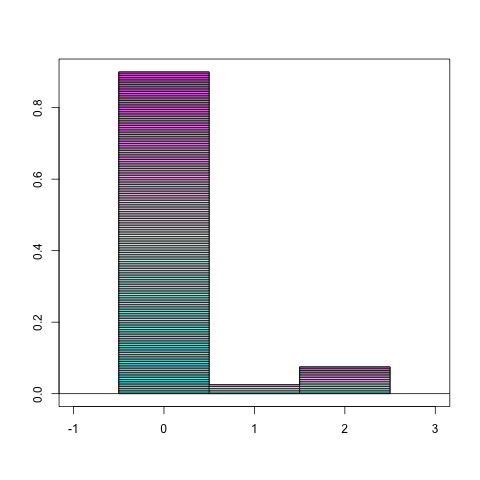
\includegraphics[width=12cm,height=10cm]{img/repProdB}
\end{center}


\item Il convient alors d'augmenter la taille d'échantillon et de sélectionner dans son nouveau échantillon les 50 premiers individus de son échantillon original. Qu'aurait-il pu en conclure~(rédaction standard)?

 
\IndicR
\begin{Verbatim}[frame=leftline,fontfamily=tt,fontshape=n,numbers=left]
> y50
 [1] 0 0 0 0 0 0 0 0 0 0 0 0 0 0 0 0 0 0 0 0 0 2 0 0 0 0 0 0 2 2 2 0 0 0 0 0 0 0
[39] 0 0 1 0 0 0 0 0 0 0 0 0
> mean(y50)
[1] 0.18
> # deltaEst.H0 <- (instruction R à fournir dans la rédaction)
> deltaEst.H0
[1] 0.3786397
\end{Verbatim}

 

\begin{Correction}

\noindent \textbf{Hypothèses de test} : $\mathbf{H}_0:$ $\mu^{B}=0.15$ vs {\large $\mathbf{H}_1:$ $\mu^{B}>0.15$}\\
\textbf{Statistique de test sous $\mathbf{H}_0$} :
  $$
  \Est{\delta_{\mu^{B},0.15}}{Y^{B}}= {\displaystyle \frac{\Est{\mu^{B}}{Y^{B}}-0.15}{
\Est{\sigma_{\cqlshat{\mu^{B}}}}{Y^{B}}
}} 
  \SuitApprox \mathcal{N}(0,1)
  $$
\textbf{Règle de décision} : Accepter $\mathbf{H}_1$ si 
  $\Est{\delta_{\mu^{B},0.15}}{y^{B}} > \delta^+_{lim,5\%}$\\
\noindent \textbf{Conclusion} :
puisqu'au vu des données, 
  \begin{eqnarray*}
\Est{\delta_{\mu^{B},0.15}}{y^{B}} &\NotR&\mathtt{(mean(y50)-0.15)/seMean(y50)}\simeq 0.3786397\\&\ngtr & \delta^+_{lim,5\%} \NotR \mathtt{qnorm(1-.05)}\simeq1.644854
\end{eqnarray*}
  
on ne peut pas plutôt penser (avec un risque de 5\%) que le produit B est rentable.
\end{Correction}






\end{enumerate}

\noindent \underline{Partie~II}

En Janvier 2005, cela fait un an que le produit~B a été lancé. L'industriel pense que son produit mieux connu des consommateurs est plus vendu. Il dispose déjà de l'échantillon de taille $n=1000$ obtenu en 2004 (que l'on note ici \texttt{yB04}) ayant notamment servi à estimer le nombre moyen de produit~B vendus en 2004, désormais noté $\mu^{B04}$. En 2005, il décide d'interroger les mêmes $n=1000$ individus qu'en 2004. Le jeu de données associé est noté \texttt{yB05} servant notamment  à estimer le nombre moyen $\mu^{B05}$ de produit~B vendus en 2005.

\begin{enumerate}
\item Peut-on penser au vu de ces données qu'il y a eu une augmentation moyenne de 2004 à 2005 d'au moins $0.02$ en nombre de produit(s)~B vendu(s)~(rédaction standard)? 

\IndicR
\begin{Verbatim}[frame=leftline,fontfamily=tt,fontshape=n,numbers=left]
> yB05-yB04
   [1]  0  0  0  0  0  0  0  0  0  0  0  0  1  0  0  0  1  0  0  0  0 -2  0  0
  [25]  0  1  1  0 -2 -2 -2  0  0  0  0  0  0  0  0  0 -1  0  0  3  0  0  0  0
...
 [961]  0  0  0 -1  0  0  0  0  0  0  1  0  0  0  0  0  0  0 -1 -2  0  1  0  0
 [985]  0  0  0  0  3  1  0  0  0  0  0  0  0  0  0  0
> mean(yB05-yB04)
[1] 0.085
> # deltaEst.H0 <- (instruction R à fournir dans la rédaction)
> pnorm(deltaEst.H0)
[1] 0.991839
\end{Verbatim}

 

\begin{Correction}
\noindent \textbf{Préliminaire}~: puisque  $\mathtt{(mean(yB05-yB04)-0.02)}\simeq0.065$ est du même signe (i.e. positif que $\mathtt{deltaEst.H0}$ (car p-valeur gauche supérieure à $50\%$), on a~:
    \begin{itemize}
\item \textit{variable d'intérêt}~: $Y^{D}=Y^{B05}-Y^{B04}$
\item \textit{paramètre d'intérêt}~: $\mu^{D}=\mbox{``moyenne de $Y^{D}$"}=\mu^{B05}-\mu^{B04}$
\end{itemize}
\noindent \textbf{Hypothèses de test} : $\mathbf{H}_0:$ $\mu^{D}=0.02$ vs {\large $\mathbf{H}_1:$ $\mu^{D}>0.02$}\\
\textbf{Statistique de test sous $\mathbf{H}_0$} :
  $$
  \Est{\delta_{\mu^{D},0.02}}{Y^{D}}= {\displaystyle \frac{\Est{\mu^{D}}{Y^{D}}-0.02}{
\Est{\sigma_{\cqlshat{\mu^{D}}}}{Y^{D}}
}} 
  \SuitApprox \mathcal{N}(0,1)
  $$
\textbf{Règle de décision} : Accepter $\mathbf{H}_1$ si 
  p-valeur (droite) < 5\%\\
\noindent \textbf{Conclusion} :
puisqu'au vu des données, 
  \[
p-valeur\NotR\mathtt{1-pnorm((mean(yB05-yB04)-0.02)/seMean(yB05-yB04))} \simeq 0.82\% < 5\%,
\]
on peut plutôt penser (avec un risque de 5\%) que le produit B est rentable.
\end{Correction}




\item En fait, après réflexion, il réalise qu'il dispose  en 2005 de la valeur de $\mu^{B04}$ égale à $0.19$. Reformulez l'assertion d'intérêt et proposez l'instruction \texttt{R} fournissant la p-valeur associée.


\end{enumerate}

\noindent \underline{Partie~III}

Souhaitant exporter le produit~B en Allemagne, l'industriel se crée un échantillon de taille $n=500$ individus, consommateurs potentiels du produit~B allemands. Il souhaite alors comparer les deux pays. Ce nouveau jeu de données est noté \texttt{yAll}

On notera $\mu^{All}$ et $\sigma^2_{All}$ les moyennes et variances des réponses des consommateurs potentiels allemands. Pour simplifier, on notera $\mu^{Fr}$ et $\sigma^2_{Fr}$  les moyennes et variances des réponses des consommateurs potentiels français, et l'échantillon de taille 1000 est noté \texttt{yFr}. 

A partir des instructions \texttt{R} ci-dessous, combien d'assertions d'intérêt différentes (en précisant lesquelles) peut-on confirmer avec les données~?

\begin{Verbatim}[frame=leftline,fontfamily=tt,fontshape=n,numbers=left]
> (mean(yFr)-mean(yAll)-0.045)/seDMean(yFr,yAll)
[1] 1.821887
> pnorm((var(yFr)/var(yAll)-2)/seRVar(yFr,yAll))
[1] 0.996465
> pnorm((var(yAll)/var(yFr)-.5)/seRVar(yAll,yFr))
[1] 1.967895e-05
\end{Verbatim}



\end{exercice}

\appendix\chapter{Représentations\\graphiques~dans~l'A.E.P.}\label{TdAEPGraph}



\begin{exercice}[Histogramme continu] ${ }$\label{ex:histMoyUnifs}
Cet exercice fait suite à l'exercice~\ref{ex:sommeUnifs} mais dans l'esprit de l'exercice~\ref{ex:loiMoyenne} puisqu'on s'intéresse à la moyenne plutôt que la somme. Voici 4 graphiques représentant les histogrammes continus des $m=200$, 2000, 5000, 10000 premières réalisations de la variable $M_2:=\frac{Y_1+Y_2}2=\frac{S}2$. Nous rappelons que les $m=10000$ réalisations de $S$ avaient été stockées dans le vecteur \texttt{s} en \texttt{R}. Les $m=10000$ réalisations $\dataEmp[m]{m_{2,[\cdot]}}$ de $M_2$ sont donc accessibles en \texttt{R} via l'instruction \texttt{s/2}. 







\centerline{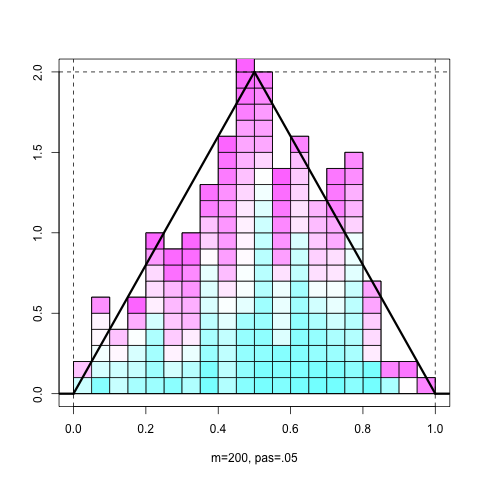
\includegraphics[width=8cm,height=8cm]{img/deuxUnif200} 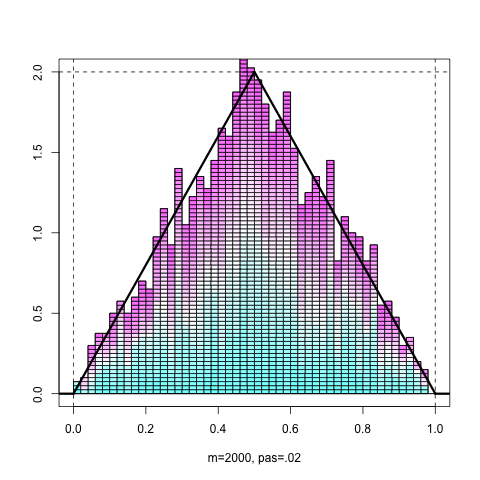
\includegraphics[width=8cm,height=8cm]{img/deuxUnif2000}}
\centerline{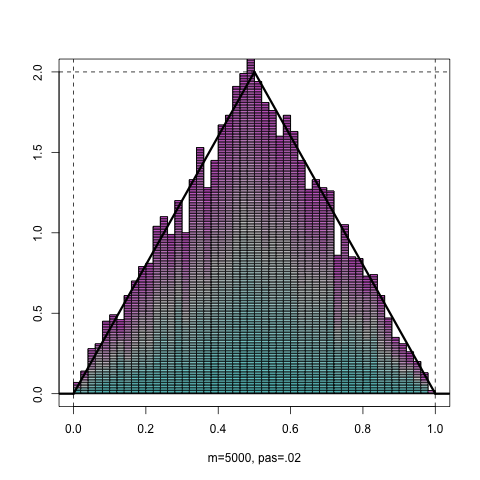
\includegraphics[width=8cm,height=8cm]{img/deuxUnif5000} 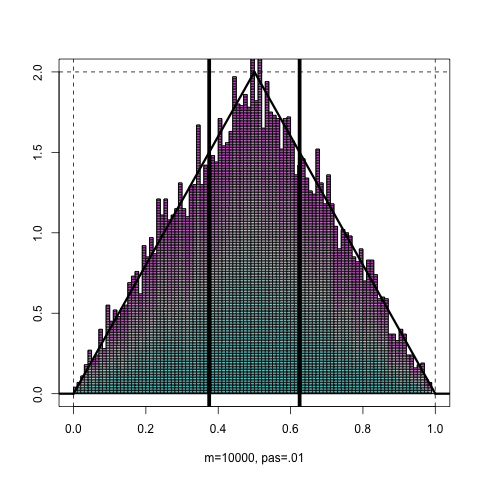
\includegraphics[width=8cm,height=8cm]{img/deuxUnif10000}}
Dans le contexte de l'\textbf{A.E.P.}, les intervalles d'un histogramme continu peuvent sans restriction être de même largeur (car $m$ est censé être suffisamment grand). 
Le ``pas" d'un histogramme nomme en général la largeur du plus petit de ces intervalles.
\begin{enumerate}
\item Pour chaque graphique, indiquez quelle est la surface d'une brique.  
\item Lequel de ces graphiques est le plus informatif~? A partir de ce dernier, êtes-vous en mesure de déterminer les valeurs de $M_2$ qui sont les plus probables~?
\item  Identifiez les briques associées aux valeurs comprises entre $\frac38$ et $\frac58$ incluses. Quelle est la valeur de l'aire de la surface occupée par ces briques en vous rappelant que la proportion des $\dataEmp[m]{m_{2,[\cdot]}}$ comprises entre $\frac38$ et $\frac58$  est fourni par~:\\
\begin{Verbatim}[frame=leftline,fontfamily=tt,fontshape=n,numbers=left]
> mean(3/8<=s/2 &  s/2<=5/8)
[1] 0.4262
\end{Verbatim}

\item Sauriez-vous alors évaluer approximativement la probabilité $\PPP{M_2\in [\frac38,\frac58]}$~?
\item Est-il possible d'évaluer approximativement $\PPP{M_2=\frac12}$ qui via l'\textbf{A.E.P.} est approchée grâce à~:
\begin{Verbatim}[frame=leftline,fontfamily=tt,fontshape=n,numbers=left]
> mean(s/2==1/2)
[1] 0
\end{Verbatim}

Que faudrait-il faire pour pouvoir y arriver~?
\item En s'imaginant que le pas $\to0$ au fur et à mesure que $m\to+\infty$, pouvez-vous décrire à quoi ressemblera une brique~? Même question pour le mur de briques~? Représentez-le sur le graphique en ne dessinant que le ``dessus" (i.e. contour supérieur) du mur. Vu comme une fonction, comment interprèteriez-vous le contour supérieur du mur~?  

\item Un mathématicien, sollicité pour nous assister dans l'étude de l'\textbf{A.M.P.}, nous apprend qu'il est classique de caractériser le comportement aléatoire de $M_2$ en fournissant la densité de probabilité (qui porte bien son nom!) s'exprimant ici mathématiquement par~:
\[
f_{M_2}(t)=\left\{\begin{array}{ll}
4t & \mbox{si }t\in [0,\frac12]\\
4-4t & \mbox{si }t\in [\frac12,1]\\
0 & \mbox{sinon}
\end{array}\right.
\]
Représentez cette fonction sur le dernier graphique et comparez-la avec les histogrammes continus. Sont-ils très différents de la fonction~?
\item Le mathématicien nous annonce que  $\PPP{M_2\in [\frac38,\frac58]}=\displaystyle\int_{\frac38}^{\frac58} f_{M_2}(t)dt$ qui est représentée graphiquement par la surface des points sous la courbe $f_{M_2}(t)$ et dont les abscisses sont compris entre $\frac38$ et $\frac58$. Représentez alors $\PPP{M_2\in [\frac38,\frac58]}$ sur le graphique. Cela ne vous rappelle pas quelquechose~?
Sachant qu'il n'est pas difficile de montrer que $\PPP{M_2\in [\frac38,\frac58]}=\PPP{S\in [\frac34,\frac54]}=\frac7{16}\simeq 43.75\%$ (déjà évaluée à l'exercice~\ref{ex:sommeUnifs}), évaluez l'aire de la surface représentant cette probabilité. 
\item Quelle est la valeur exacte de $\PPP{M_2=\frac12}$~?
\item Sélectionnez la bonne réponse parmi les réponses (proposées en suivant entre parenthèses)~:\\
La modalité $\frac12$ est le mode de la loi de $M_2$ car $\frac12$ est la valeur qui maximise la fonction \underline{\hspace*{1cm}} ( $\mathbf{p_{M_2}(x)}:=\PPP{M_2=x}$ ou $\mathbf{f_{M_2}(x)}$ ou $\mathbf{F_{M_2}(x)}:=\PPP{M_2\leq x}$ ).
Cela se traduit littéralement par~: $\frac12$ est la valeur de plus grande \underline{\hspace*{2cm}}( \textbf{probabilité} ou \textbf{densité de probabilité} ou \textbf{fonction de répartition} ).

\end{enumerate}
\end{exercice}
\begin{exercice}[Histogramme discret] ${ }$\label{ex:histMoyDes}
On s'intéresse à la loi de probabilité de la moyenne $M_2:=\frac{Y_1+Y_2}2=\frac{S}2$ où $S$ représente la somme de deux dés (introduite auparavant à l'exercice~\ref{ex:sommeDes}). Le but est ici d'introduire la notion d'histogramme discret qui n'est pas la représentation graphique la plus usuelle pour représenter une variable aléatoire discrète. Voici 4 histogrammes discrets pour les $m=200$, 1000, 2000 et 5000 premières somme des deux dés. Remarquons que dans le cadre de l'exercice, nous aurions pu nous limiter à la représentation graphique usuelle en diagramme en bâton
puisque nous n'aurons aucune intention de comparer la loi de probabilité de $M_2$ avec celle d'une loi de probabilité associée à une variable aléatoire continue. Ce sera en revanche le cas dans l'exercice~\ref{ex:histMoyenne}.
    








Afin de mettre en avant les caractéristiques les distinguant des histogrammes continus, nous avons complété les histogrammes en identifiant les modalités de $M_2$ par des petits traits en gras sur l'axe des abscisses prolongés par des lignes verticales en trait pointillé.

\centerline{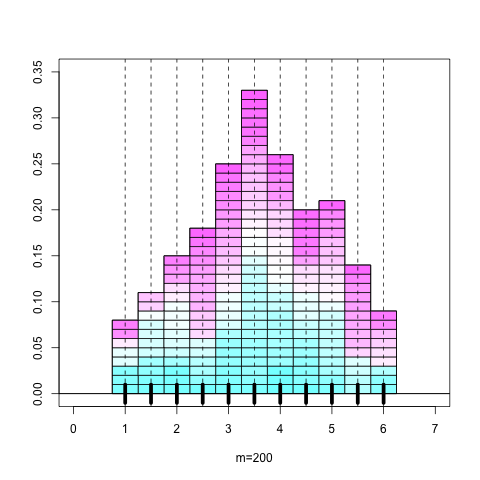
\includegraphics[width=8cm,height=8cm]{img/deuxDes200} 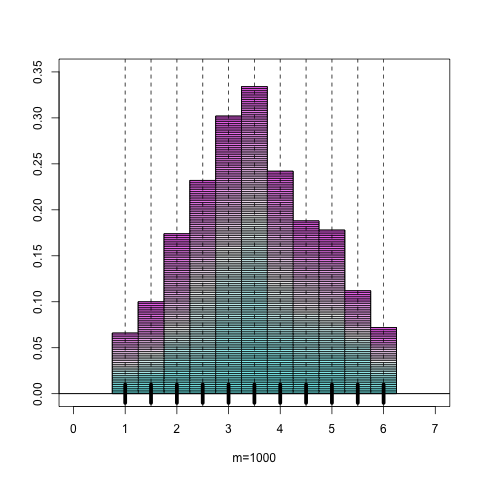
\includegraphics[width=8cm,height=8cm]{img/deuxDes1000}}
\centerline{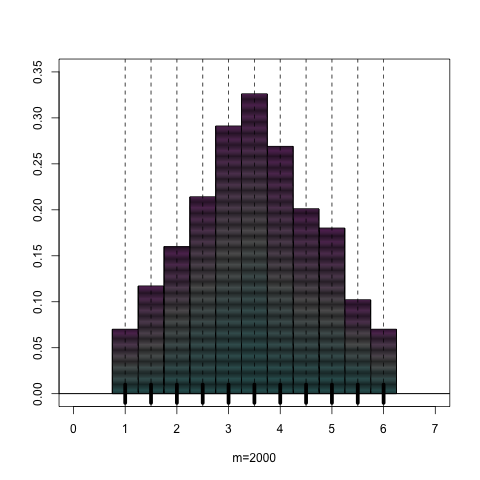
\includegraphics[width=8cm,height=8cm]{img/deuxDes2000} 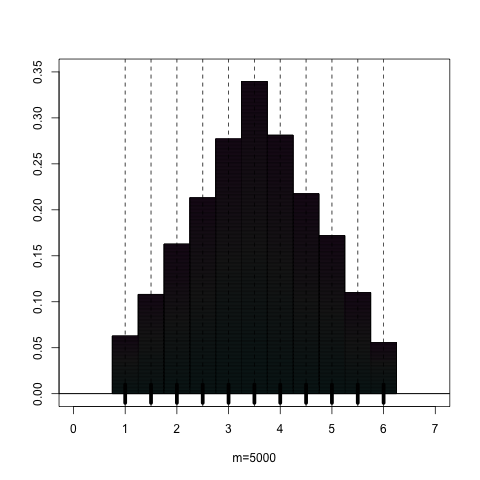
\includegraphics[width=8cm,height=8cm]{img/deuxDes5000}}


\begin{enumerate}
\item Quelles sont les largeurs des briques utilisées dans ces histogrammes discrets~? Changent-elles lorsque $m$ augmente (justifier votre réponse)~? Sur chacun des graphiques, indiquez l'aire de la surface de chaque brique. 
\item A partir du premier graphique, donnez un ordre de grandeur de la probabilité $\PPP{M_2=1}$. Quelle est l'aire de la surface occupée par les briques associées aux $m_{2,[k]}=1$~? A-t'on vraiment besoin de voir les briques individuellement pour évaluer $\PPP{M_2=1}$~? Si vous avez répondu non, appliquez cela sur le dernier graphique puisque les briques ne sont pas distinguables individuellement tellement elles sont plates.
\item Le graphique suivant fournit deux histogrammes discrets l'un correspondant à $m=5000$ et l'autre à celui $m\to+\infty$. Deux types de trait (simple et en gras) ont été utilisés pour les représenter. Sauriez-vous les identifier~? Evaluez (le plus précisément possible) $\PPP{M_2=1}$ ainsi que $\PPP{M_2\in\{1,1.5,6\}}$.
      

\centerline{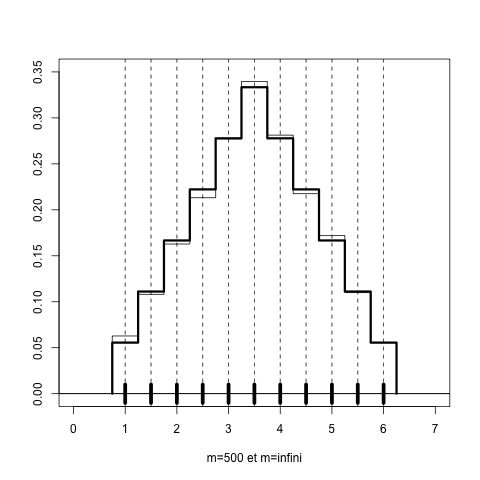
\includegraphics[width=8cm,height=8cm]{img/deuxDesInf}}
\end{enumerate}
\end{exercice}
\begin{Indication}{A retenir}
\noindent $\to$ L'histogramme discret s'interprète de la même manière qu'un histogramme continu où les probabilités (ou proportions) sont mesurées via des aires de surfaces.\\
\noindent $\to$ A la différence d'un histogramme continu, dans un histogramme discret~:
\begin{itemize} 
\item les briques sont de largeur fixe (même lorsque $m$ varie)
\item la base d'une brique n'a pas vraiment de sens
\item seul le centre de la base d'une brique a un sens puisqu'il indique la valeur associée qui se lit en abscisse (surtout si la brique n'est pas la première à avoir été empilée).  
\end{itemize} 
\end{Indication}
\begin{exercice}[Histogramme de moyenne] ${ }$ \label{ex:histMoyenne}
L'étude menée est la suite de l'exercice~\ref{ex:loiMoyenne}. Ayant introduit les notions d'histogrammes discret et continu, nous allons pouvoir apprécier de visualiser le théorème de la limite centrale notamment dans le cadre de l'exemple de la moyenne de dés. Voici pour commencer, 2 graphiques représentant les contours supérieurs des histogrammes (discrets pour l'exemple du dé à gauche et continu pour l'exemple de la loi uniforme sur $[1,6]$ à droite) des lois de probabilité $M_n$ pour $n=1,2,4,16,64$. Les échelles sont identiques pour les 2 graphiques.














































\centerline{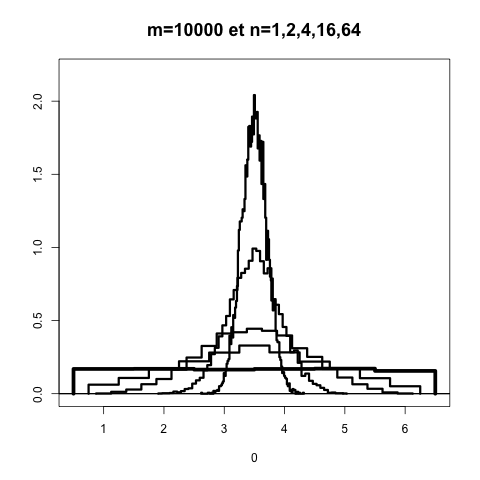
\includegraphics[width=8cm,height=8cm]{img/moyDes}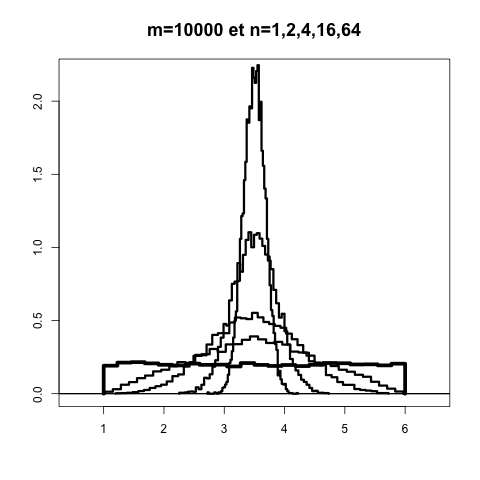
\includegraphics[width=8cm,height=8cm]{img/moyUnifs}}

\begin{enumerate}
\item Pour chaque graphique, quelle est l'histogramme qui représente via l'\textbf{A.E.P.} la loi de probabilité approximative de $Y_1$~? 
\item Ces représentations graphiques expriment-elles le résultat que nous avions décrit sur le procédé de moyennisation qui concentre les modalités~?
\item Comparez les 2 graphiques. Pour quelle étude (dé ou uniforme), la moyenne est de plus grande variance~?
\item Sauriez-vous anticiper les histogrammes pour le cas où $n\to+\infty$ avec $m\to+\infty$~?
\item Comme il n'est pas possible d'observer la forme de l'histogramme dans le cas précédent, il est naturel de faire comme un photographe en rezoomant le graphique de sorte à pouvoir mieux cadrer l'histogramme sur le graphique. C'est aussi ce que fait automatiquement le logiciel~\texttt{R} comme on peut le voir dans la série de graphiques suivants~:\\[0.25cm]
\hspace*{-2.3cm}\begin{tabular}{|c|c|c|c|}\hline
\multicolumn{2}{|c|}{Exemple du dé: $Y_i\leadsto \mathcal{U}(\{1,2,3,4,5,6\})$} & \multicolumn{2}{c|}{Exemple de l'uniforme: $Y_i\leadsto \mathcal{U}([1,6])$}\\\hline
loi de $M_n$ & loi de $\Delta_n$ & loi de $M_n$ & loi de $\Delta_n$\\\hline
%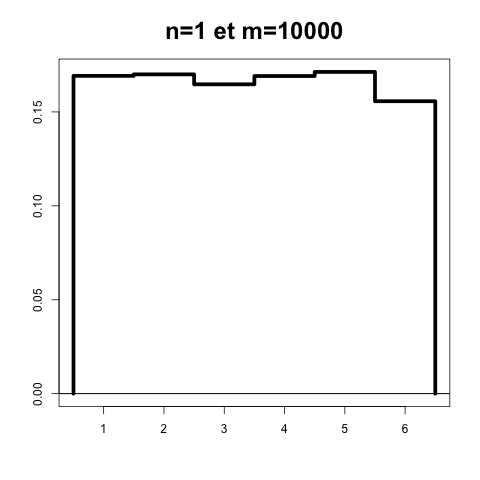
\includegraphics[width=4cm,height=4cm]{img/n1MoyDes} & 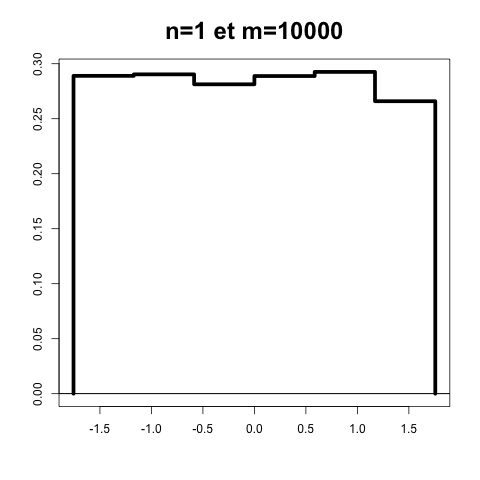
\includegraphics[width=4cm,height=4cm]{img/n1DeltaMoyDes} & 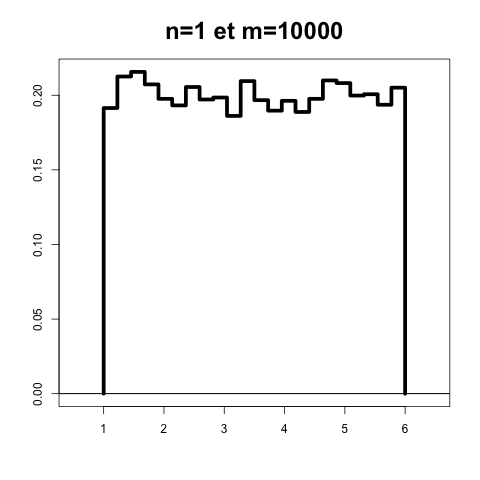
\includegraphics[width=4cm,height=4cm]{img/n1MoyUnifs} & 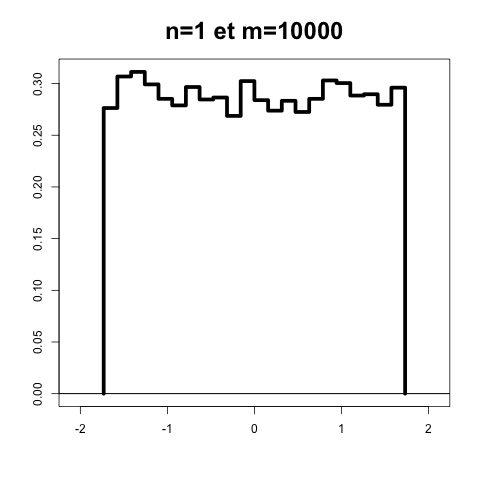
\includegraphics[width=4cm,height=4cm]{img/n1DeltaMoyUnifs}\\\hline
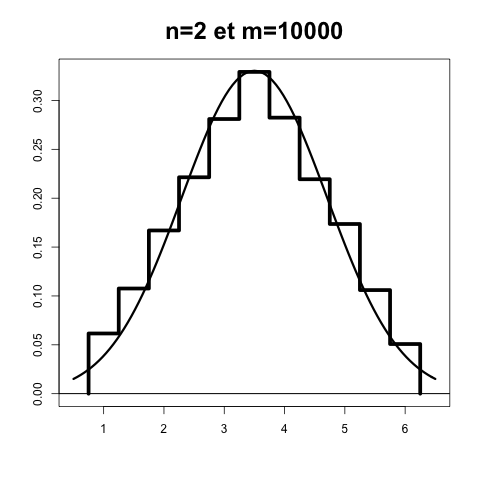
\includegraphics[width=4cm,height=4cm]{img/n2MoyDes} & 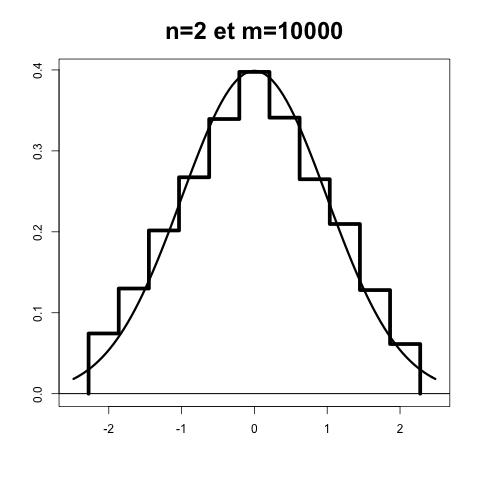
\includegraphics[width=4cm,height=4cm]{img/n2DeltaMoyDes} & 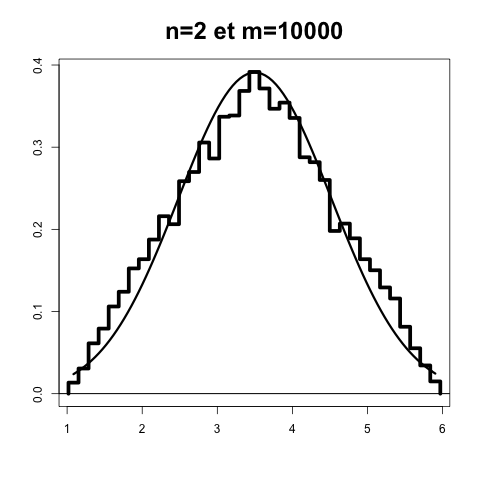
\includegraphics[width=4cm,height=4cm]{img/n2MoyUnifs} & 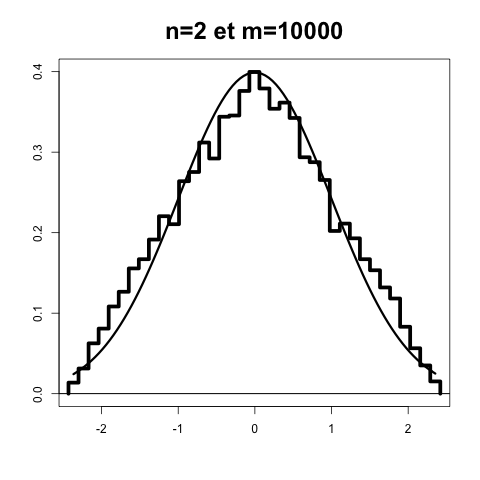
\includegraphics[width=4cm,height=4cm]{img/n2DeltaMoyUnifs}\\\hline
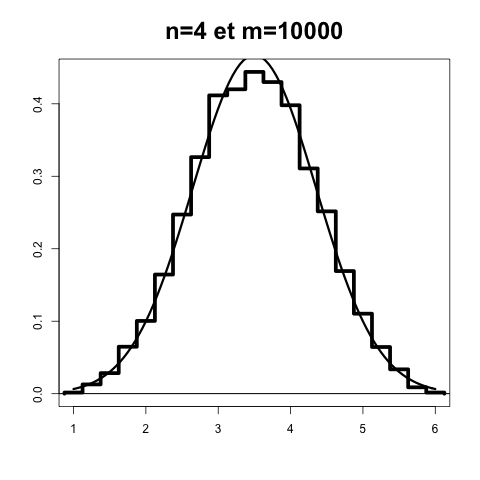
\includegraphics[width=4cm,height=4cm]{img/n4MoyDes} & 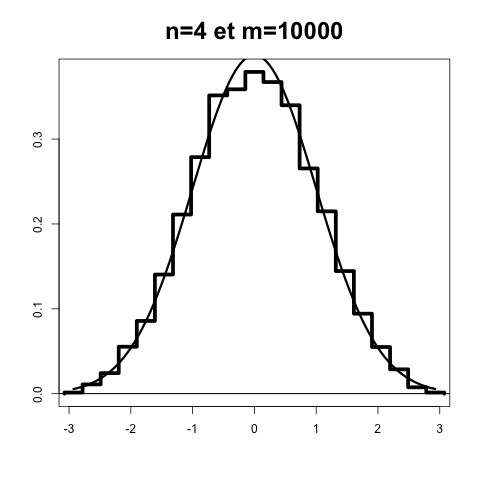
\includegraphics[width=4cm,height=4cm]{img/n4DeltaMoyDes} & 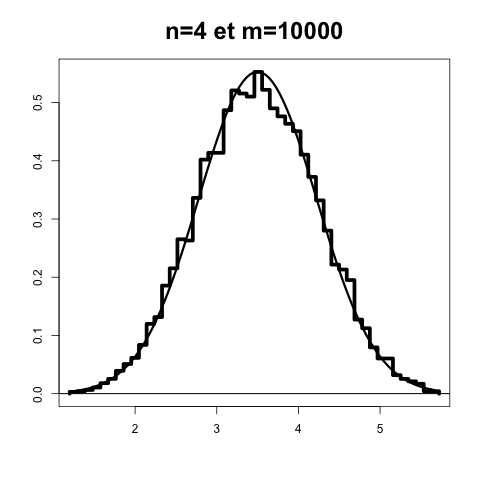
\includegraphics[width=4cm,height=4cm]{img/n4MoyUnifs} & 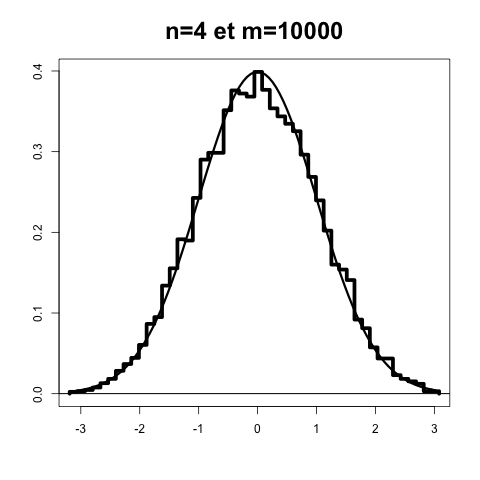
\includegraphics[width=4cm,height=4cm]{img/n4DeltaMoyUnifs}\\\hline
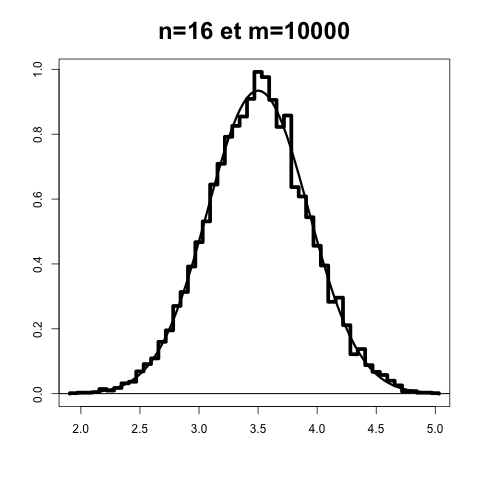
\includegraphics[width=4cm,height=4cm]{img/n16MoyDes} & 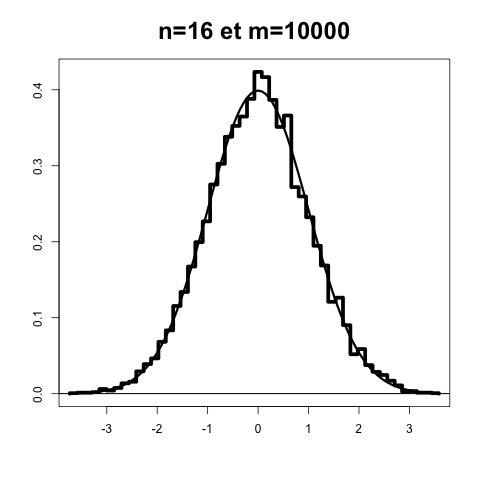
\includegraphics[width=4cm,height=4cm]{img/n16DeltaMoyDes} & 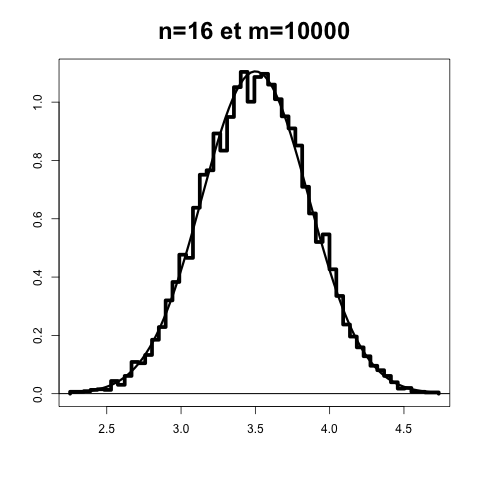
\includegraphics[width=4cm,height=4cm]{img/n16MoyUnifs} & 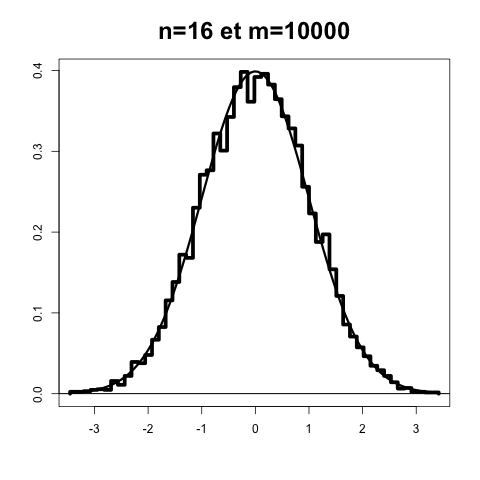
\includegraphics[width=4cm,height=4cm]{img/n16DeltaMoyUnifs}\\\hline
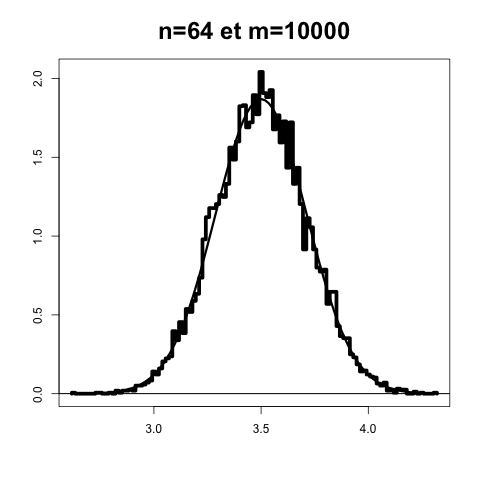
\includegraphics[width=4cm,height=4cm]{img/n64MoyDes} & 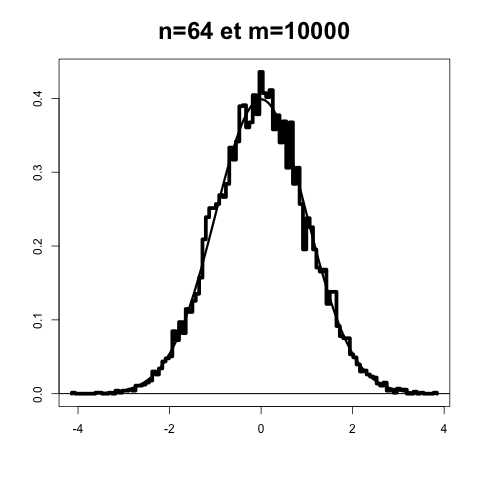
\includegraphics[width=4cm,height=4cm]{img/n64DeltaMoyDes} & 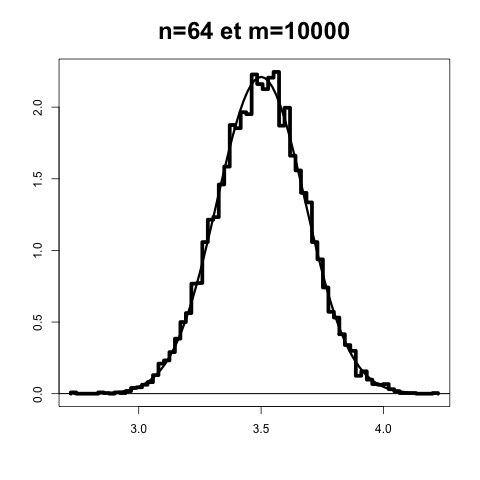
\includegraphics[width=4cm,height=4cm]{img/n64MoyUnifs} & 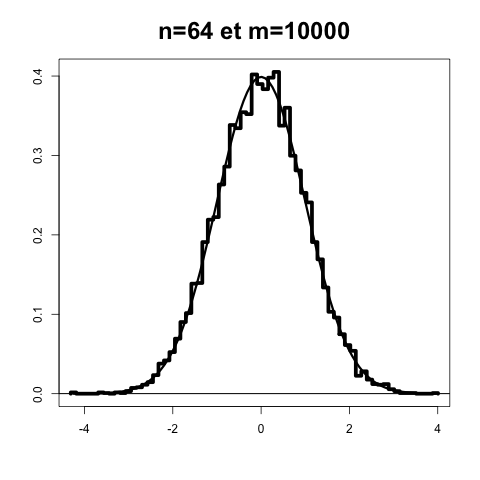
\includegraphics[width=4cm,height=4cm]{img/n64DeltaMoyUnifs}\\\hline
\end{tabular}
\item Pour les 2 exemples et pour chaque $n$, comparez la forme de l'histogramme (en trait le plus épais) des réalisations de $M_n$ avec celle de l'histogramme (en trait le plus épais) des réalisations $\Delta_n$~? Expliquez pourquoi il en est ainsi~?
\item Pourquoi ces histogrammes sont-ils de plus en plus irréguliers lorsque $n$ augmente~? Qu'aurait dû faire l'expérimentateur pour qu'il n'en soit pas ainsi~? Pouvez-vous tout de même imaginer ce qui ce serait passé lorsque $m\to+\infty$~?
\item D'après le Théorème de la limite centrale, on peut mathématiquement affirmer, lorsque $n$ est suffisamment grand (convention simplifiée appliquée dans ce cours: $n\geq 30$)~:
\[
  M_n\SuitApprox \mathcal{N}\left(\EEE{Y_1},\sqrt{\frac{\VVV{Y_1}}{n}}\right) \Leftrightarrow \Delta_n:=\frac{M_n-\EEE{Y_1}}{\sqrt{\frac{\VVV{Y_1}}{n}}} \SuitApprox \mathcal{N}(0,1).
\]
Aussi, on rappelle que, pour l'exemple du dé, $\VVV{Y_1}=2.9167$ et que, pour l'exemple de la loi uniforme sur $[1,6]$,  $\VVV{Y_1}=\frac{25}{12}$.\\
Pour chaque graphique, que représente la courbe en trait le plus fin~?  Est-elle de plus en plus ressemblante à l'histogramme en trait le plus épais lorsque $n$ augmente (Indication~: éviter de tenir compte du caractère irrégulier de l'histogramme quand $n$ augmente uniquement dû au fait que $m$ aurait dû être augmenté en même temps que $n$)~?
\item Dans le contexte de l'\textbf{A.E.P.}, comment décririez-vous ces courbes~? %répartitions de m=+\infty de \mathcal{N}\left(\EEE{Y_1},\sqrt{\frac{\VVV{Y_1}}{n}}\right)
Dans l'exemple du dé, les deux histogrammes représentées sur chaque graphique sont-ils de la même nature~? Avez-vous une idée sur comment illustrer graphiquement le Théorème de la limite centrale sans l'utilisation de l'histogramme discret (\textit{Indication}~: Une réponse très courte est bien venue)~?  
\item Le Théorème de la limite centrale s'appliquant pour tout $Y_1$ ayant n'importe quelle loi de probabilité admettant une moyenne et une variance finies, imaginez la même série de graphiques que précédemment mais pour d'autres exemples que ceux (uniformes) choisis dans cette étude.   
\end{enumerate}

\end{exercice}






\end{document}


